\documentclass[12pt,twoside,a4paper,openright]{report}
\usepackage{etex}
% Select encoding of your inputs.
\usepackage[utf8]{inputenc}

% Make latex understand and use the typographic
% rules of the language used in the document.
\usepackage[english, danish]{babel}

% Use the vector font Latin Modern which is going
% to be the default font in latex in the future.
\usepackage{lmodern}

% Choose the font encoding
\usepackage[T1]{fontenc}

% Use colour in tables
\usepackage[table]{xcolor}
\usepackage{array}
\usepackage{multirow}

% load a colour package
\usepackage{xcolor}
\definecolor{aaublue}{RGB}{33,26,82}% dark blue

% The standard graphics inclusion package
\definecolor{white}{RGB}{255,255,255} % define color white
\usepackage{graphicx}
\usepackage{adjustbox}

% Set up how figure and table captions are displayed
\usepackage{caption}
\captionsetup{
  font=footnotesize,% set font size to footnotesize
  labelfont=bf % bold label (e.g., Figure 3.2) font
}

% Enable row combination in tables
\usepackage{multirow}

% Make space between table lines and text
\renewcommand{\arraystretch}{1.5}

% Make the standard latex tables look so much better
\usepackage{array,booktabs}

% Enable the use of frames around, e.g., theorems
% The framed package is used in the example environment
\usepackage{framed}
\usepackage{colortbl}
\usepackage{longtable}
\usepackage{xcolor}
\usepackage{textcomp}

%%%%%%%%%%%%%%%%%%%%%%%%%%%%%%%%%%%%%%%%%%%%%%%%
% Mathematics
%%%%%%%%%%%%%%%%%%%%%%%%%%%%%%%%%%%%%%%%%%%%%%%%
% Defines new environments such as equation,
% align and split 
\usepackage{amsmath}
\usepackage{relsize}
% Adds new math symbols
\usepackage{amssymb}
% Use theorems in your document
% The ntheorem package is also used for the example environment
% When using thmmarks, amsmath must be an option as well. Otherwise \eqref doesn't work anymore.
\usepackage[framed,amsmath,thmmarks]{ntheorem}
\usepackage{cancel}

%%%%%%%%%%%%%%%%%%%%%%%%%%%%%%%%%%%%%%%%%%%%%%%%
% Page Layout
%%%%%%%%%%%%%%%%%%%%%%%%%%%%%%%%%%%%%%%%%%%%%%%%
% Change margins, papersize, etc of the document
\usepackage[
  left=25mm,% left margin on an odd page %tidligere 25mm for baade right og left
  right=25mm,% right margin on an odd page
  top=35mm,
  ]{geometry}
  
% Modify how \chapter, \section, etc. look
% The titlesec package is very configureable
\usepackage{titlesec}
\makeatletter
\def\ttl@mkchap@i#1#2#3#4#5#6#7{%
    \ttl@assign\@tempskipa#3\relax\beforetitleunit
    \vspace{\@tempskipa}%<<<<<< REMOVE THE * AFTER \vspace
    \global\@afterindenttrue
    \ifcase#5 \global\@afterindentfalse\fi
    \ttl@assign\@tempskipb#4\relax\aftertitleunit
    \ttl@topmode{\@tempskipb}{%
        \ttl@select{#6}{#1}{#2}{#7}}%
    \ttl@finmarks  % Outside the box!
    \@ifundefined{ttlp@#6}{}{\ttlp@write{#6}}}
\makeatother

\titlespacing{\chapter}{0pt}{0pt}{10pt}
\titlespacing{\section}{0pt}{0pt}{-5pt}
\titlespacing{\subsection}{0pt}{8pt}{-5pt}
\titlespacing{\subsubsection}{0pt}{6pt}{-10pt}

\titleformat*{\section}{\normalfont\Large\bfseries\color{aaublue}}
\titleformat*{\subsection}{\normalfont\large\bfseries\color{aaublue}}
\titleformat*{\subsubsection}{\normalfont\normalsize\bfseries\color{aaublue}}

\usepackage{bookmark}
\usepackage{titlesec, blindtext, color}
%\color{gray75}{gray}{0.75}
\newcommand{\hsp}{\hspace{20pt}}
\titleformat{\chapter}[hang]{\Huge\bfseries}{\thechapter\hsp\textcolor{aaublue}{|}\hsp}{0pt}{\Huge\bfseries}

% Change the headers and footers
\usepackage{fancyhdr}
\setlength{\headheight}{15pt}
\pagestyle{fancy}
\fancyhf{} %delete everything
\renewcommand{\headrulewidth}{0pt} %remove the horizontal line in the header
\fancyhead[RO,LE]{\color{aaublue}\small\nouppercase\leftmark} %even page - chapter title
\fancyhead[LO]{}
\fancyhead[RE]{} 
\fancyhead[CE]{}
\fancyhead[CO]{}
\fancyfoot[RE,LO]{\thepage}
\fancyfoot[LE,RO]{} %page number on all pages
\fancyfoot[CE,CO]{}

% change first page of all chapters header and footer to fancy style
\makeatletter
\let\ps@plain\ps@fancy
\makeatother

% Do not stretch the content of a page. Instead,
% insert white space at the bottom of the page
\raggedbottom

% Enable arithmetics with length. Useful when typesetting the layout.
\usepackage{calc}

%%%%%%%%%%%%%%%%%%%%%%%%%%%%%%%%%%%%%%%%%%%%%%%%
% Bibliography
%%%%%%%%%%%%%%%%%%%%%%%%%%%%%%%%%%%%%%%%%%%%%%%%
%setting references (using numbers) and supporting i.a. Chicargo-style:
\usepackage{etex}
\usepackage{etoolbox}
\usepackage{keyval}
\usepackage{ifthen}
\usepackage{url}
\usepackage{csquotes}
\usepackage[backend=biber, url=true, doi=true, style=numeric, sorting=none]{biblatex}
\addbibresource{setup/bibliography.bib}

%%%%%%%%%%%%%%%%%%%%%%%%%%%%%%%%%%%%%%%%%%%%%%%%
% Misc
%%%%%%%%%%%%%%%%%%%%%%%%%%%%%%%%%%%%%%%%%%%%%%%%

%%% Enables the use FiXme refferences. Syntax: \fxnote{...} %%%
\usepackage[footnote, draft, english, silent, nomargin]{fixme}
%With "final" instead of "draft" an error will ocure for every FiXme under compilation.

%%% allows use of lorem ipsum (generate i.e. pagagraph 1 to 5 with \lipsum[1-5]) %%%
\usepackage{lipsum}

%%% Enables figures with text wrapped tightly around it %%%
\usepackage{wrapfig}

%%% Section debth included in table of contents (1 = down to sections) %%%
\setcounter{tocdepth}{1}

%%% Section debth for numbers (1 = down to sections) %%%
\setcounter{secnumdepth}{1}

\usepackage{tocloft}
\setlength{\cftbeforetoctitleskip}{0 cm}
\renewcommand{\cftpartpresnum}{Part~}
\let\cftoldpartfont\cftpartfont
\renewcommand{\cftpartfont}{\cftoldpartfont\cftpartpresnum}

%%%%%%%%%%%%%%%%%%%%%%%%%%%%%%%%%%%%%%%%%%%%%%%%
% Hyperlinks
%%%%%%%%%%%%%%%%%%%%%%%%%%%%%%%%%%%%%%%%%%%%%%%%

% Enable hyperlinks and insert info into the pdf
% file. Hypperref should be loaded as one of the 
% last packages
\usepackage{nameref}
\usepackage{hyperref}
\hypersetup{%
	%pdfpagelabels=true,%
	plainpages=false,%
	pdfauthor={Author(s)},%
	pdftitle={Title},%
	pdfsubject={Subject},%
	bookmarksnumbered=true,%
	colorlinks,%
	citecolor=aaublue,%
	filecolor=aaublue,%
	linkcolor=aaublue,% you should probably change this to black before printing
	urlcolor=aaublue,%
	pdfstartview=FitH%
}

% remove all indentations
\setlength\parindent{0pt}
\parskip 5mm
\usepackage{verbatim}

\definecolor{Gra}{RGB}{230,230,230}

%creates a nice-looking C#-text
\newcommand{\CC}{C\nolinebreak\hspace{-.05em}\raisebox{.3ex}{\scriptsize\text \#} }

%enables multi column lists
\usepackage{multicol}

%enables code-examples
\usepackage{listings}

\definecolor{coolblue}{RGB}{32,95,128}
\definecolor{mygreen}{rgb}{0,0.6,0}
\definecolor{mygray}{rgb}{0.5,0.5,0.5}
\definecolor{mymauve}{rgb}{0.58,0,0.82}
\usepackage{textcomp}
\definecolor{listinggray}{gray}{0.9}
\definecolor{lbcolor}{rgb}{0.9,0.9,0.9}

\lstdefinestyle{customcpp}{
    backgroundcolor=\color{lbcolor},
    tabsize=4,
    rulecolor=,
    language=C++,
    basicstyle=\scriptsize,
    upquote=true,
    aboveskip={1.5\baselineskip},
    columns=fixed,
    showstringspaces=false,
    extendedchars=true,
    breaklines=true,
    prebreak = \raisebox{0ex}[0ex][0ex]{\ensuremath{\hookleftarrow}},
    frame=single,
    showtabs=false,
    numbers=left,
    captionpos=b,
    numbersep=5pt,
    numberstyle=\tiny\color{mygray},
    showspaces=false,
    showstringspaces=false,
    identifierstyle=\ttfamily,
    keywordstyle=\color[rgb]{0,0,1},
    commentstyle=\color[rgb]{0.133,0.545,0.133},
    stringstyle=\color[rgb]{0.627,0.126,0.941},
}
\lstdefinestyle{custommatlab}{
    backgroundcolor=\color{lbcolor},
    tabsize=4,
    rulecolor=,
    language=Matlab,
    basicstyle=\scriptsize,
    upquote=true,
    aboveskip={1.5\baselineskip},
    columns=fixed,
    showstringspaces=false,
    extendedchars=true,
    breaklines=true,
    prebreak = \raisebox{0ex}[0ex][0ex]{\ensuremath{\hookleftarrow}},
    frame=single,
    showtabs=false,
    numbers=left,
    captionpos=b,
    numbersep=5pt,
    numberstyle=\tiny\color{mygray},
    showspaces=false,
    showstringspaces=false,
    identifierstyle=\ttfamily,
    keywordstyle=\color[rgb]{0,0,1},
    commentstyle=\color[rgb]{0.133,0.545,0.133},
    stringstyle=\color[rgb]{0.627,0.126,0.941},   
}
\lstdefinestyle{custommatlabinline}{
    style=custommatlab,
    basicstyle=\small,
}
\lstdefinestyle{customcppinline}{
    style=customcpp,
    basicstyle=\small,
}
\lstset{
%  backgroundcolor=\color{white},   % choose the background color; you must add \usepackage{color} or \usepackage{xcolor}
%  basicstyle=\footnotesize,        % the size of the fonts that are used for the code
%  breakatwhitespace=false,         % sets if automatic breaks should only happen at whitespace
%  breaklines=true,                 % sets automatic line breaking
%  captionpos=t,                    % sets the caption-position to bottom
%  commentstyle=\color{mygreen},    % comment style
%  deletekeywords={...},            % if you want to delete keywords from the given language
%  escapeinside={\%*}{*)},          % if you want to add LaTeX within your code
%  extendedchars=true,              % lets you use non-ASCII characters; for 8-bits encodings only, does not work with UTF-8
%  frame=single,                    % adds a frame around the code
%  keepspaces=true,                 % keeps spaces in text, useful for keeping indentation of code (possibly needs columns=flexible)
%  keywordstyle=\color{blue},       % keyword style
%  language=C++,                 % the language of the code
%  morekeywords={*,...},            % if you want to add more keywords to the set
%  numbers=left,                    % where to put the line-numbers; possible values are (none, left, right)
%  numbersep=5pt,                   % how far the line-numbers are from the code
%  numberstyle=\tiny\color{mygray}, % the style that is used for the line-numbers
%  rulecolor=\color{black},         % if not set, the frame-color may be changed on line-breaks within not-black text (e.g. comments (green here))
%  showspaces=false,                % show spaces everywhere adding particular underscores; it overrides 'showstringspaces'
%  showstringspaces=false,          % underline spaces within strings only
%  showtabs=false,                  % show tabs within strings adding particular underscores
%  stepnumber=1,                    % the step between two line-numbers. If it's 1, each line will be numbered
%  stringstyle=\color{mymauve},     % string literal style
%  tabsize=2,                       % sets default tabsize to 2 spaces
%  title=\lstname                   % show the filename of files included with \lstinputlisting; also try caption instead of title
    style=customcpp
}

\usepackage{float}
\usepackage{caption}
\usepackage{subcaption}
\usepackage{siunitx}
\sisetup{decimalsymbol=comma}
\sisetup{detect-weight}

\usepackage{enumitem}
%\usepackage[citestyle=authoryear,natbib=true]{biblatex}

% Figures - TIKZ
\usepackage{tikz}
\usetikzlibrary{shapes,arrows}
\usepackage[americanresistors,americaninductors,americancurrents, americanvoltages]{circuitikz}

% Wall of text logo
\newcommand{\walloftextalert}[0]{\includegraphics[width=\textwidth]{walloftext.png}}

\usepackage{pdfpages}
\usepackage{lastpage}
\usepackage{epstopdf}

\setlength{\headheight}{21pt}

\hfuzz=\maxdimen
\tolerance = 10000
\hbadness  = 10000

\usepackage{siunitx}
\graphicspath{{./figures/}}% package inclusion and set up of the document

%%%%%%%%%%%%%%%%%%%%%%%%%%%%%%%%%%%%%%%%%%%%%%%%%%%%%
%             UNITS, EQUATIONS AND TEXT             %
%%%%%%%%%%%%%%%%%%%%%%%%%%%%%%%%%%%%%%%%%%%%%%%%%%%%%
%Units:
\newcommand{\unit}[1]{&& \left[\si{#1}\right]} %\newcommand{\unit}[1]{[\si{#1}]}             <<| Use these if you want equations to be
\newcommand{\unitWh}[1]{[\si{#1}]}             %\newcommand{\eq}[2]{&&\si{#1} &= \si{#2}&&}  <<| centered.. .. will appear scrambled
\newcommand{\numUnit}[1]{\ \si{#1}&}           %                                               | from one equation to the next though..
%Equation:                                     %                                               | and does not work with long equations.. :/
\newcommand{\eq}[2]{\si{#1} &= \si{#2}}
\newcommand{\arw}{&& &\Updownarrow&&}
\newcommand{\eqOne}[2]{\si{#1} &= \si{#2} &\nonumber\\}
\newcommand{\eqTwo}[1]{&\ \ \ \ \si{#1}&}
%Text:
\newcommand{\tx}[1]{\text{#1}}
%Vectors
\renewcommand{\vec}[1]{\boldsymbol{\mathbf{#1}}}
%Vertical line in equations ie. |_x=y (whereTwo stacks two equalities at the line)
\newcommand{\where}[1]{ \left.\rule{0cm}{.5cm}\right\vert\rule{0cm}{.4cm}_{\substack{\rule{0cm}{.15cm}\\ \si{#1} }} }
\newcommand{\whereTwo}[2]{ \left.\rule{0cm}{.67cm}\right\vert\rule{0cm}{.5cm}_{\substack{\si{#1} \rule{0cm}{.19cm}\\\vspace{-.1cm}\\ \si{#2}}} }

%%%%%%%%%%%%%%%%%%%%%%%%%%%%%%%%%%%%%%%%%%%%%%%%%%%%%
%                 TIKZ SETTINGS                     %
%%%%%%%%%%%%%%%%%%%%%%%%%%%%%%%%%%%%%%%%%%%%%%%%%%%%%
\usetikzlibrary{arrows.meta}
\tikzset{
  block/.style    = {draw, thick, rectangle,
                     minimum height = 2.1em,
                     minimum width = 1.7em},
  sum/.style      = {draw, circle, inner sep=1.5pt},
}

%%%%%%%%%%%%%%%%%%%%%%%%%%%%%%%%%%%%%%%%%%%%%%%%%%%%%
%                  REFERENCES                       %
%%%%%%%%%%%%%%%%%%%%%%%%%%%%%%%%%%%%%%%%%%%%%%%%%%%%%

%Chapter
\newcommand{\Chapref}[1]{\emph{Chapter \ref{#1}}}
\newcommand{\chapref}[1]{\emph{chapter \ref{#1}}}
%Section
\newcommand{\Secref}[1]{\emph{Section \ref{#1}}}
\newcommand{\secref}[1]{\emph{section \ref{#1}}}
%subSection
\newcommand{\Subsecref}[1]{\emph{Subsection \ref{#1}}}
\newcommand{\subsecref}[1]{\emph{subsection \ref{#1}}}
%Appendix
\newcommand{\Appref}[1]{\emph{Appendix \ref{#1}}}
\newcommand{\appref}[1]{\emph{appendix \ref{#1}}}
%Listings
\newcommand{\Coderef}[1]{\emph{Listings: \ref{#1}}}
\newcommand{\coderef}[1]{\emph{listings: \ref{#1}}}
%Figure:
\newcommand{\Figref}[1]{\emph{Figure \ref{#1}}}
\newcommand{\figref}[1]{\emph{figure \ref{#1}}}
%Table:
\newcommand{\Tableref}[1]{\emph{Table \ref{#1}}}
\newcommand{\tableref}[1]{\emph{table \ref{#1}}}

%Expressions:
\newcommand{\Expr}[1]{\emph{Expression (\ref{#1})}}
\newcommand{\expr}[1]{\emph{expression (\ref{#1})}}

%Equations:
%1 equation:
\newcommand{\Eqref}[1]{\emph{Equation (\ref{#1})}}
\renewcommand{\eqref}[1]{\emph{equation (\ref{#1})}}
%2 equations:
\newcommand{\EqrefTwo}[2]{\emph{Equation (\ref{#1})} and \emph{(\ref{#2})}}
\newcommand{\eqrefTwo}[2]{\emph{equation (\ref{#1})} and \emph{(\ref{#2})}}
%3 equations:
\newcommand{\EqrefThree}[3]{\emph{Equation (\ref{#1})}, \emph{(\ref{#2})} and \emph{(\ref{#3})}}
\newcommand{\eqrefThree}[3]{\emph{equation (\ref{#1})}, \emph{(\ref{#2})} and \emph{(\ref{#3})}}
%4 equations:
\newcommand{\EqrefFour}[4]{\emph{Equation (\ref{#1})}, \emph{(\ref{#2})}, \emph{(\ref{#3})} and \emph{(\ref{#4})}}
\newcommand{\eqrefFour}[4]{\emph{equation (\ref{#1})}, \emph{(\ref{#2})}, \emph{(\ref{#3})} and \emph{(\ref{#4})}}
%5 equations:
\newcommand{\EqrefFive}[5]{\emph{Equation (\ref{#1})}, \emph{(\ref{#2})}, \emph{(\ref{#3})}, \emph{(\ref{#4})} and \emph{(\ref{#5})}}
\newcommand{\eqrefFive}[5]{\emph{equation (\ref{#1})}, \emph{(\ref{#2})}, \emph{(\ref{#3})}, \emph{(\ref{#4})} and \emph{(\ref{#5})}}
%6 equations:
\newcommand{\EqrefSix}[6]{\emph{Equation (\ref{#1})}, \emph{(\ref{#2})}, \emph{(\ref{#3})}, \emph{(\ref{#4})}, \emph{(\ref{#5})} and \emph{(\ref{#6})}}
\newcommand{\eqrefSix}[6]{\emph{equation (\ref{#1})}, \emph{(\ref{#2})}, \emph{(\ref{#3})}, \emph{(\ref{#4})}, \emph{(\ref{#5})} and \emph{(\ref{#6})}}
%7 equations:
\newcommand{\EqrefSeven}[7]{\emph{Equation (\ref{#1})}, \emph{(\ref{#2})}, \emph{(\ref{#3})}, \emph{(\ref{#4})}, \emph{(\ref{#5})}, \emph{(\ref{#6})} and \emph{(\ref{#7})}}
\newcommand{\eqrefSeven}[7]{\emph{equation (\ref{#1})}, \emph{(\ref{#2})}, \emph{(\ref{#3})}, \emph{(\ref{#4})}, \emph{(\ref{#5})}, \emph{(\ref{#6})} and \emph{(\ref{#7})}}% my new macros

%\toggleNotes{on}

\begin{document}
	%%% Prereport %%%
	\setlength\cftaftertoctitleskip{2pt}
	\setlength\cftafterloftitleskip{6pt}
	\setlength\cftafterlottitleskip{6pt}
	\selectlanguage{english}
	\title{Quadcopter}
	
	%%% Frontmatter Settings %%%
	\pagestyle{empty} %disable headers and footers
	\pagenumbering{roman} %use roman page numbering in the frontmatter I II...
	\fancyfoot[RE,LO]{16gr733} %page number on all pages
	\fancyfoot[LE,RO]{\thepage}
	\fancyhead[LE,LO,RE,RO]{}
	
	%%% Introductory Formalities %%%
	\pdfbookmark[0]{Front Page}{label:forside}%
\begin{titlepage}
  \addtolength{\hoffset}{0.5\evensidemargin-0.5\oddsidemargin} %set equal margins on the frontpage - remove this line if you want default margins
  \noindent%
  \begin{tabular}{@{}p{\textwidth}@{}}
    \toprule[2pt]
    \midrule
    \vspace{0.2cm}
    \begin{center}
    \Huge{\textbf{
      Stabilization of a Quadcopter % insert your title here
    }}
    \end{center}
    \begin{center}
      \Large{

      }
    \end{center}
    \vspace{0.2cm}\\
    \midrule
    \toprule[2pt]
  \end{tabular}
   \vspace{0.55 cm}
  \begin{figure}[!ht]
\centering
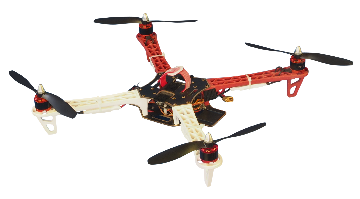
\includegraphics[width=0.8\textwidth]{figures/quadcopter}
\label{fig:forside}
\end{figure}
  \vspace{0.6 cm}
  \begin{center}
    {\large
      7. Semester Project Worksheets %Insert document type (e.g., Project Report)
    }\\
    \vspace{0.2cm}
    {\Large
      Group 16gr733%Insert your group name or real names here
    }
  \end{center}
  \begin{center}
  Aalborg University\\
  Electronic Engineering \& IT\\
  Fredrik Bajers Vej 7\\
  DK-9220 Aalborg
  \end{center}
\end{titlepage}

\clearpage
	\pagestyle{fancy}
	%\small
%\begin{figure}[H] 
%	\centering
%	\includegraphics[scale=0.38]{figures/Cubli-7}
%\end{figure}\vspace{-18pt}\begin{figure}[H] 
%	\centering
%	\includegraphics[scale=0.4]{figures/Cubli-2}
%\end{figure}\vspace{-18pt}\begin{figure}[H] 
%	\centering
%	\includegraphics[scale=0.3, angle=180]{figures/Cubli-3}
%\end{figure}\vspace{-18pt}\begin{figure}[H] 
%	\centering
%	\includegraphics[scale=0.4, angle=180]{figures/Cubli-1}
%\end{figure}
\strut\vfill % push the content to the bottom of the page
\noindent Copyright \copyright{} Aalborg University 2016\par
\vspace{0.2cm}

\noindent This report is compiled in \LaTeX, originally developed by Leslie Lamport, based on Donald Knuth's \TeX. The main text is written in \emph{Latin Modern} pt 12, designed by Bogusław Jackowski and Janusz M. Nowacki. 
%The document is compiled via the website \url{www.overleaf.com}, an online collaborative based \LaTeX-editor with instant preview, which enables multiple persons to edit the document simultaneously.
Diagrams are made using Inkscape and Tikz.% Microsoft Visio. 
\clearpage
	%\begin{document} 
%\thispagestyle{empty}
%\begin{titlepage}
\begin{nopagebreak}
{\samepage 

\begin{tabular}{r}
\parbox{\textwidth}{  \raisebox{-15mm}{
\includegraphics[height=3cm]{figures/aaulogo-en.png}}
\hfill \hspace{2cm} \parbox{8cm}{\begin{tabular}{l} %4.90
{\small \textbf{\textcolor{aaublue}{\colorbox{white}{7\textsuperscript{th} Semester, Bachelor Project}}}}\\
{\small \textbf{\textcolor{aaublue}{School of Information and}}}\\
{\small \textbf{\textcolor{aaublue}{Communication Technologies}}}\\ 
{\small \textbf{\textcolor{aaublue}{}}}\\
{\small \textcolor{aaublue}{Fredrik Bajers Vej 7C}} \\
{\small \textcolor{aaublue}{9220 Aalborg}} \\
{\small \textcolor{aaublue}{\emph{http://www.sict.aau.dk/electronics-and-it}}}
\end{tabular}}}
\end{tabular}

\begin{tabular}{cc}
\parbox{7cm}{

\textbf{Title:}

Stabilization of a Quadcopter \\

\textbf{Theme:} \\
\small{
\\
}


\parbox{8cm}{


\textbf{Project Period:}\\
P7, Fall 2016\\
01/09/2016 - 22/12/2016\\
   
\textbf{Project Group:}\\
733\\ %\fxnote{Input group number}
  
\textbf{Participants:}\\
Alejandro Alonso García\\
Amalie V. Petersen\\
Andrea Victoria Tram Løvemærke\\
Niels Skov Vestergaard\\
Noelia Villarmarzo Arruñada\\

\textbf{Supervisors:}\\
}\\

\textbf{Prints:} 8\\
\textbf{Pages:} 125\\
\textbf{Appendices:} 15 (37 pages)\\
\textbf{Attached:} 1 DVD\\
\textbf{Concluded:} 25/05/2016\\

\vfill } &
\parbox{7cm}{
  \vspace{.15cm}
  \hfill
  \begin{tabular}{l}
  {\textbf{Synopsis}}\bigskip \\
  \fbox{
    \parbox{6.5cm}{\bigskip
     {\vfill{\small \lipsum[5]
     \bigskip}}
     }}
   \end{tabular}}
\end{tabular} %\vspace{1cm}
}


\textit{\phantom{A}Publication of this report's contents (including citation) without permission\\ \phantom{A}from the authors is prohibited}\\

\end{nopagebreak}
%\end{titlepage}
%\end{document}
	%%% Preface %%%
	%\cleardoublepage
	\newgeometry{left=25mm,	right=25mm, top=18mm}

\chapter*{Preface}
%\textbf{\huge{Preface}}
\lipsum[5]

\textbf{Reading Instructions}\\
\vspace{-6pt}\\
\lipsum[5]

\textbf{Text by:}\\
\vspace{-5pt}
\begin{table}[H]
	\centering
		\begin{tabular}{c c c}
			\underline{\phantom{JAERJAERJAERJAERGO}} & \phantom{cookies} & \underline{\phantom{JAERJAERJAERJAERGO}} \\
			Alejandro Alonso García			& \phantom{cookies} & Amalie V. Petersen		\\
			&&\\
			\underline{\phantom{JAERJAERJAERJAERGO}} & \phantom{cookies} & \underline{\phantom{JAERJAERJAERJAERGO}} \\
			Andrea Victoria Tram Løvemærke			& \phantom{cookies} & Niels Skov Vestergaard		\\
			&&\\
	    \multicolumn{3}{c}{\underline{\phantom{JAERJAERJAERJAERGO}}}\\
	    \multicolumn{3}{c}{Noelia Villarmarzo Arruñada}\\				
		\end{tabular}
\end{table}

\pagebreak
\restoregeometry
	
	\cleardoublepage
	
	\pdfbookmark[0]{Table of Contents}{label: tableOfContents}
	\tableofcontents
	\cleardoublepage
	
	
	%%% Mainmatter Settings %%%
	\pagenumbering{arabic} %use arabic page numbering in the mainmatter
	\fancyfoot[RO,LE]{\thepage \text{ of} \pageref{LastPage}}
	\fancyfoot[RE,LO]{16gr733}
	\fancyhead[RE,LO]{}
	\fancyhead[RE,LO]{\color{aaublue}\small\nouppercase\leftmark} %even page - chapter title
	\pagestyle{fancy}
	
	%%% Part 1 %%%
	\part{Pre-Analysis}
	
	%---------- Chapter 1 ---------------------------------------- 
	\chapter{Introduction}
Drones has a wide variety of potential uses, such as search and rescue, inspection, security, surveillance, research, aerial photography, unmanned cargo systems, military applications, the list goes on. Drones are already widely used, and while some of the aforementioned applications raises ethical issues for debate, there is no doubt that drones also hold a place in the future.

Multicopters constitutes a class of drones with fixed-pitch propellers. This means that the actuation is achieved from a difference in speed between the propellers. Among the all the different varieties of multicopters, see some examples on \autoref{fig:multicopters}, the quadcopter is the most popular, largely due to a compromise between stabilization capabilities and cost of hardware. \cite{TypesOfMulticopter}

\begin{figure}[H]
  \centering
  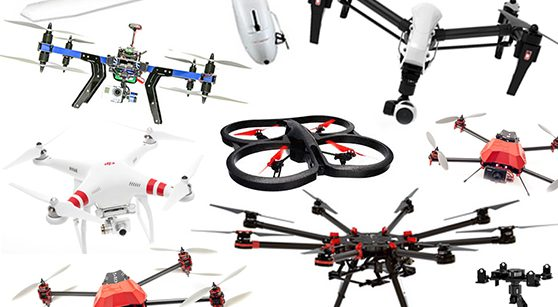
\includegraphics[width=.6\linewidth]{figures/multicopters}
  \caption{A small selection of drones which belongs to the large class of multicopters. \cite{multiCopterPhoto}}
  \label{fig:multicopters}
\end{figure}

The aim of the project is to investigate the capabilities of a specific design strategy when controlling a quadcopter as part of a distributed system.

The quadcopter obtains its attitude and position over a network from an external motion tracking system. This introduces delay and packet loss as a limiting factor to the control system situated on the quadcopter. The controlling code is implemented in C on a microcontroller using a real time operating system (RTOS), called FreeRTOS.

The system's coupled behavior and instability raises a challenging control task. This task is solved by implementing a controller design, which is based on a model derived by first principle modeling. This is later linearized since it is desired to use linear controllers.\\
The system is divided into an attitude controller and translational controllers, where the translational controllers are cascaded around the attitude controller.

The attitude control strategy is based in state space design, and makes use of state feedback, a linear quadratic regulator (LQR) and an integral controller.\\
The translational controllers are designed as classical linear proportional and integral controllers around the inner state space design.

This project provides design and realization of the described system. It results in evaluation of performance tests revealing the capabilities of the system.\\
Some interesting subjects in focus are the performance achievable using the chosen linear attitude control strategy, the influence of remote sensing on the attitude control, the influence of the attitude control bandwidth on the translational controllers and the performance of a cascaded control structure with classical linear translational controllers.


%Papers on relevant subjects:
%The performance achievable using the chosen linear attitude control strategy


%The influence of remote sensing on the attitude control


%The influence of the attitude control bandwidth on the translational controllers


%The performance of a cascaded control structure with classical linear translational controllers.







	

	%---------- Chapter 2 ---------------------------------------- 
	\chapter{System Description}
In this project a quadcopter is provided with motors, motor controllers, propellers and a battery. The system in its initial state is seen on \autoref{fig:systemBase}. Apart from the quadcopter and the attached hardware, a tracking system called Vicon is also provided. This is used to track the quadcopter and provide it with sensor inputs.

Additional to the provided hardware, an ATmega 2560 and XBEE modules are used as a processor and wireless communication modules, respectively.

\begin{figure}[H]
  \centering
  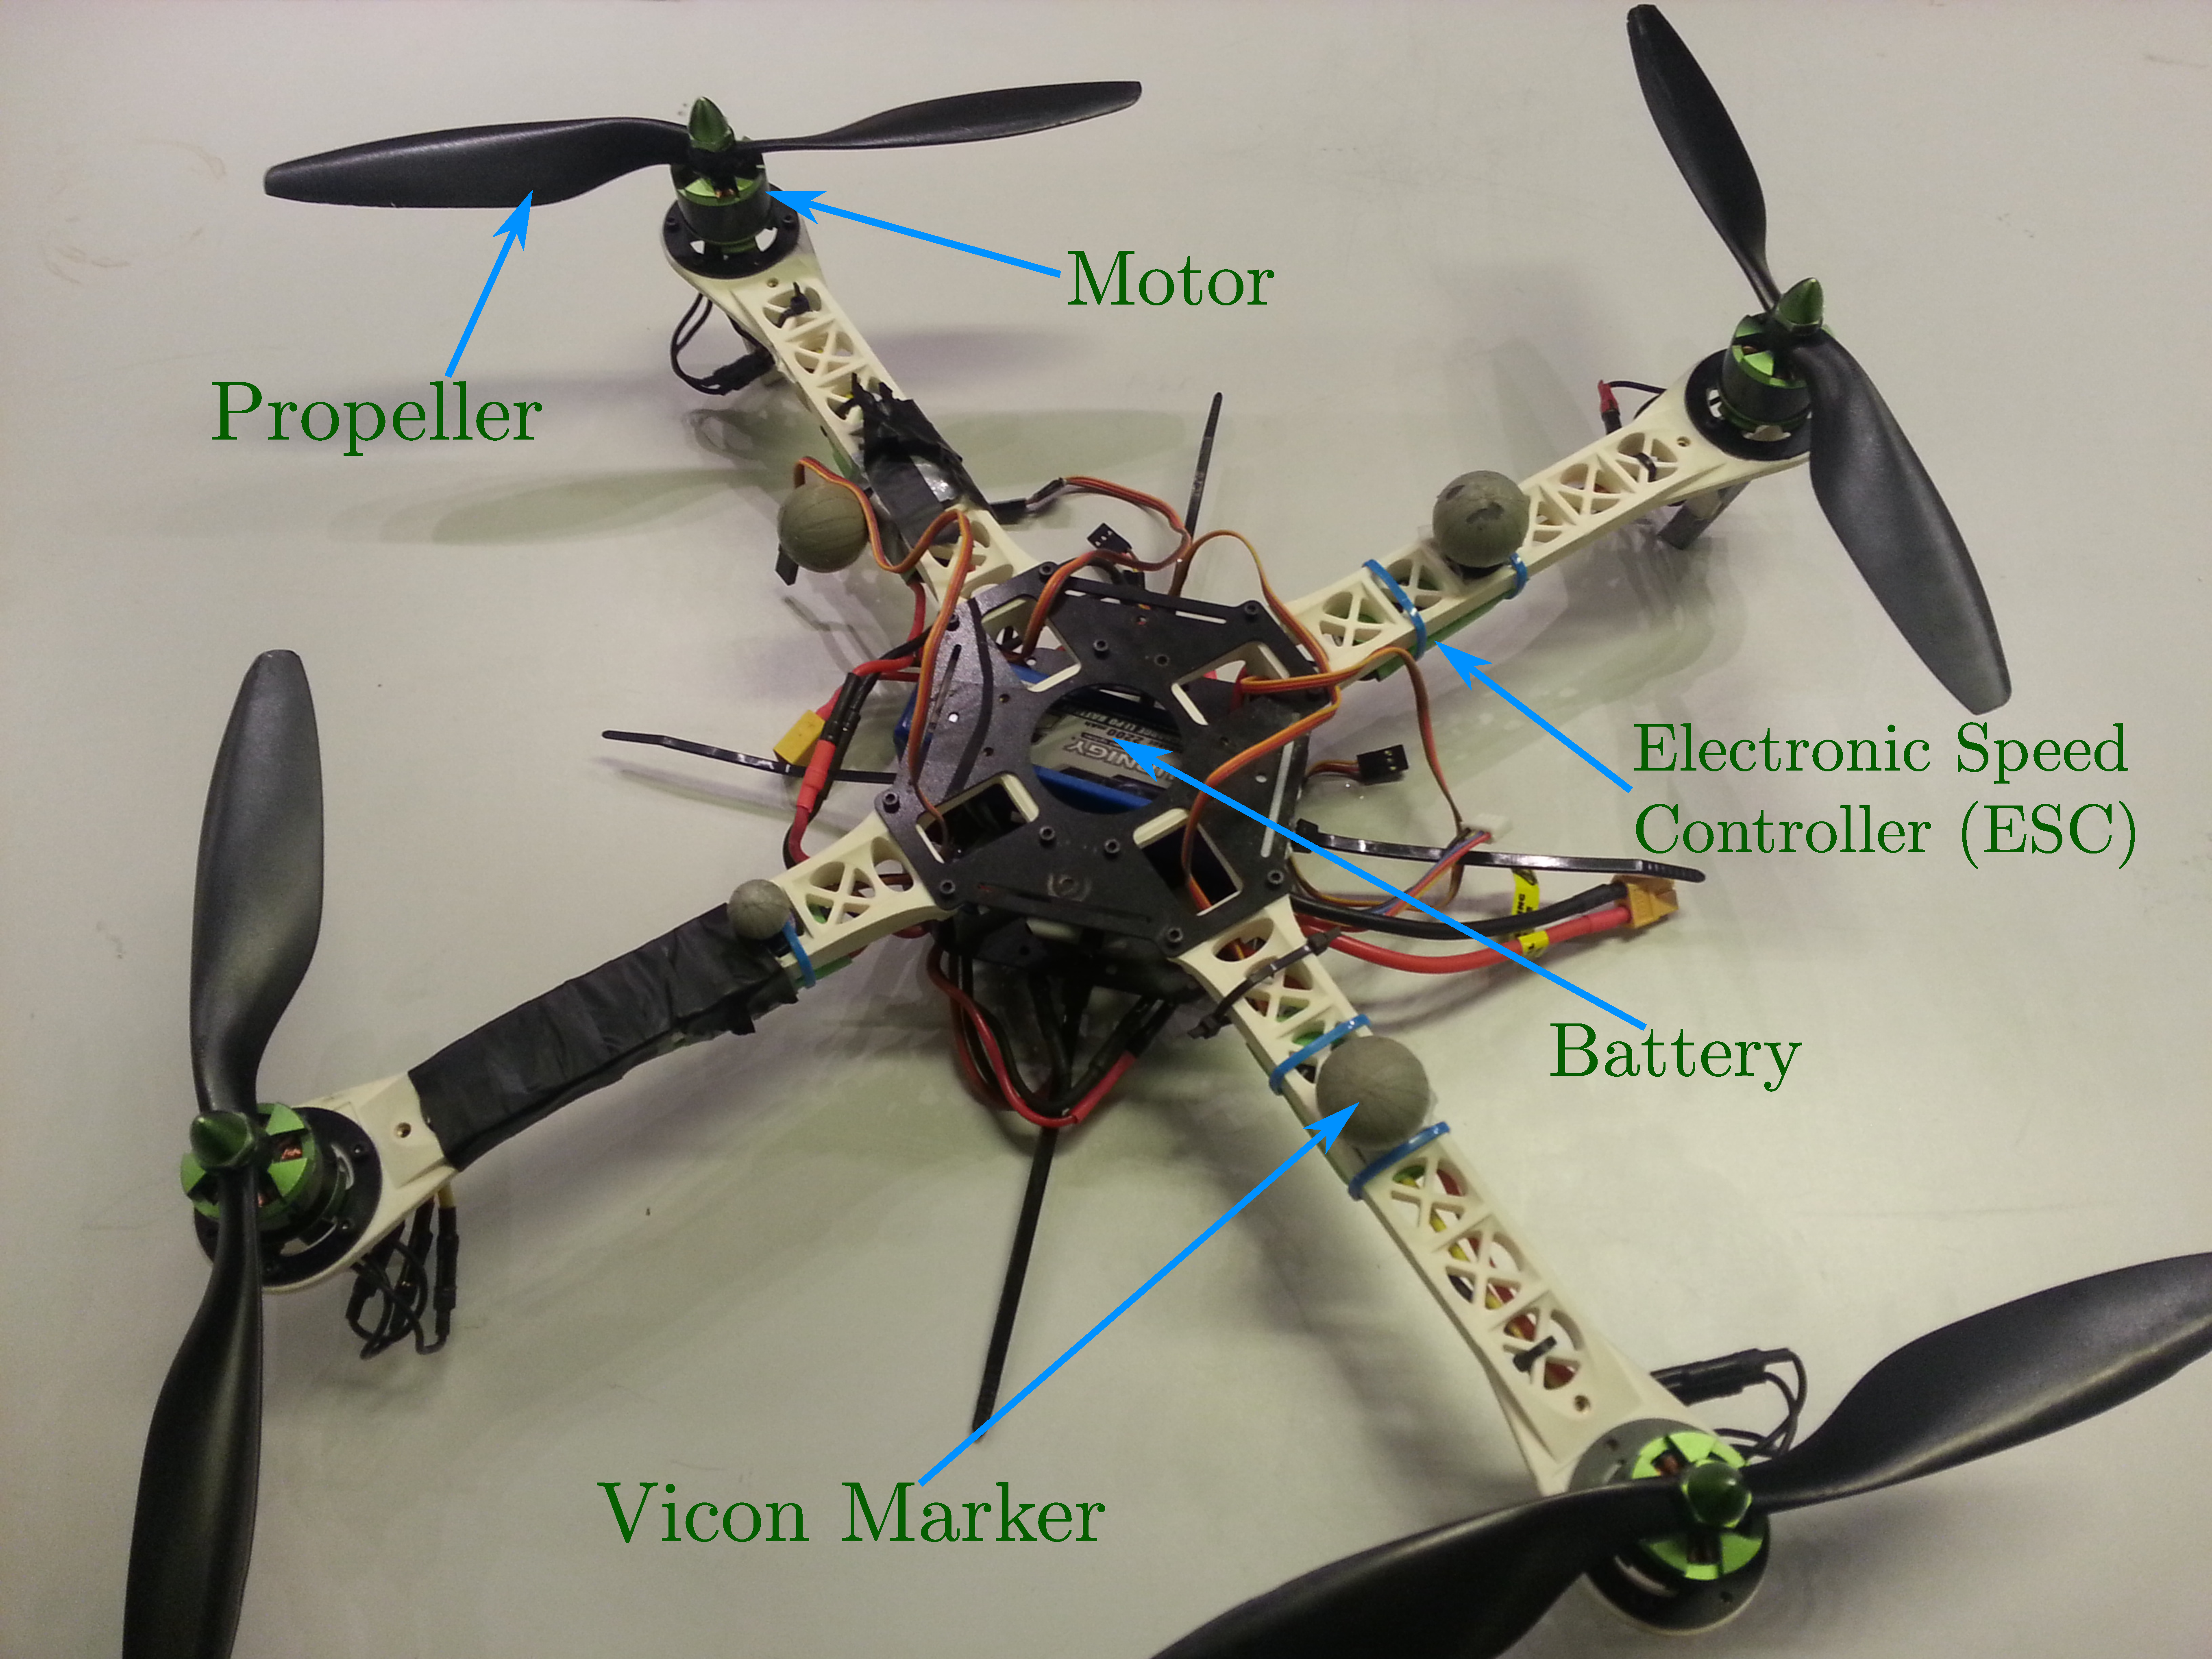
\includegraphics[width=.6\linewidth]{figures/quadcopterBaseLabels}
  \caption{The quadcopter with attached hardware as given.}
  \label{fig:systemBase}
\end{figure}

In this chapter the hardware is presented after which the overall structure of the prototype is described.
	\section{Provided hardware}\label{sec:hardware}
%The quadcopter has been provided by Aalborg university and professor Henrik Shjøiler\fixme{add danish letters}. This chapter has the purpose of describing the hardware. 
%The hardware is tested and the results of these test will be presented. 
The provided hardware is described in this section. This is with the purpose of of ensuring, that the system is well known as it sets some limits for the selected hardware as well as the design for the control system, that must make the quadcopter fly steadily.  

%The provided hardware used to develop this project consists of the quadcopter and the Vicon system that is used as a sensor. In this section, the most relevant hardware is explained in more detail. 
\cite{YDing}
The provided quadcopter can be seen in \autoref{fig:systemBase}.
\begin{figure}[H]
  \centering
  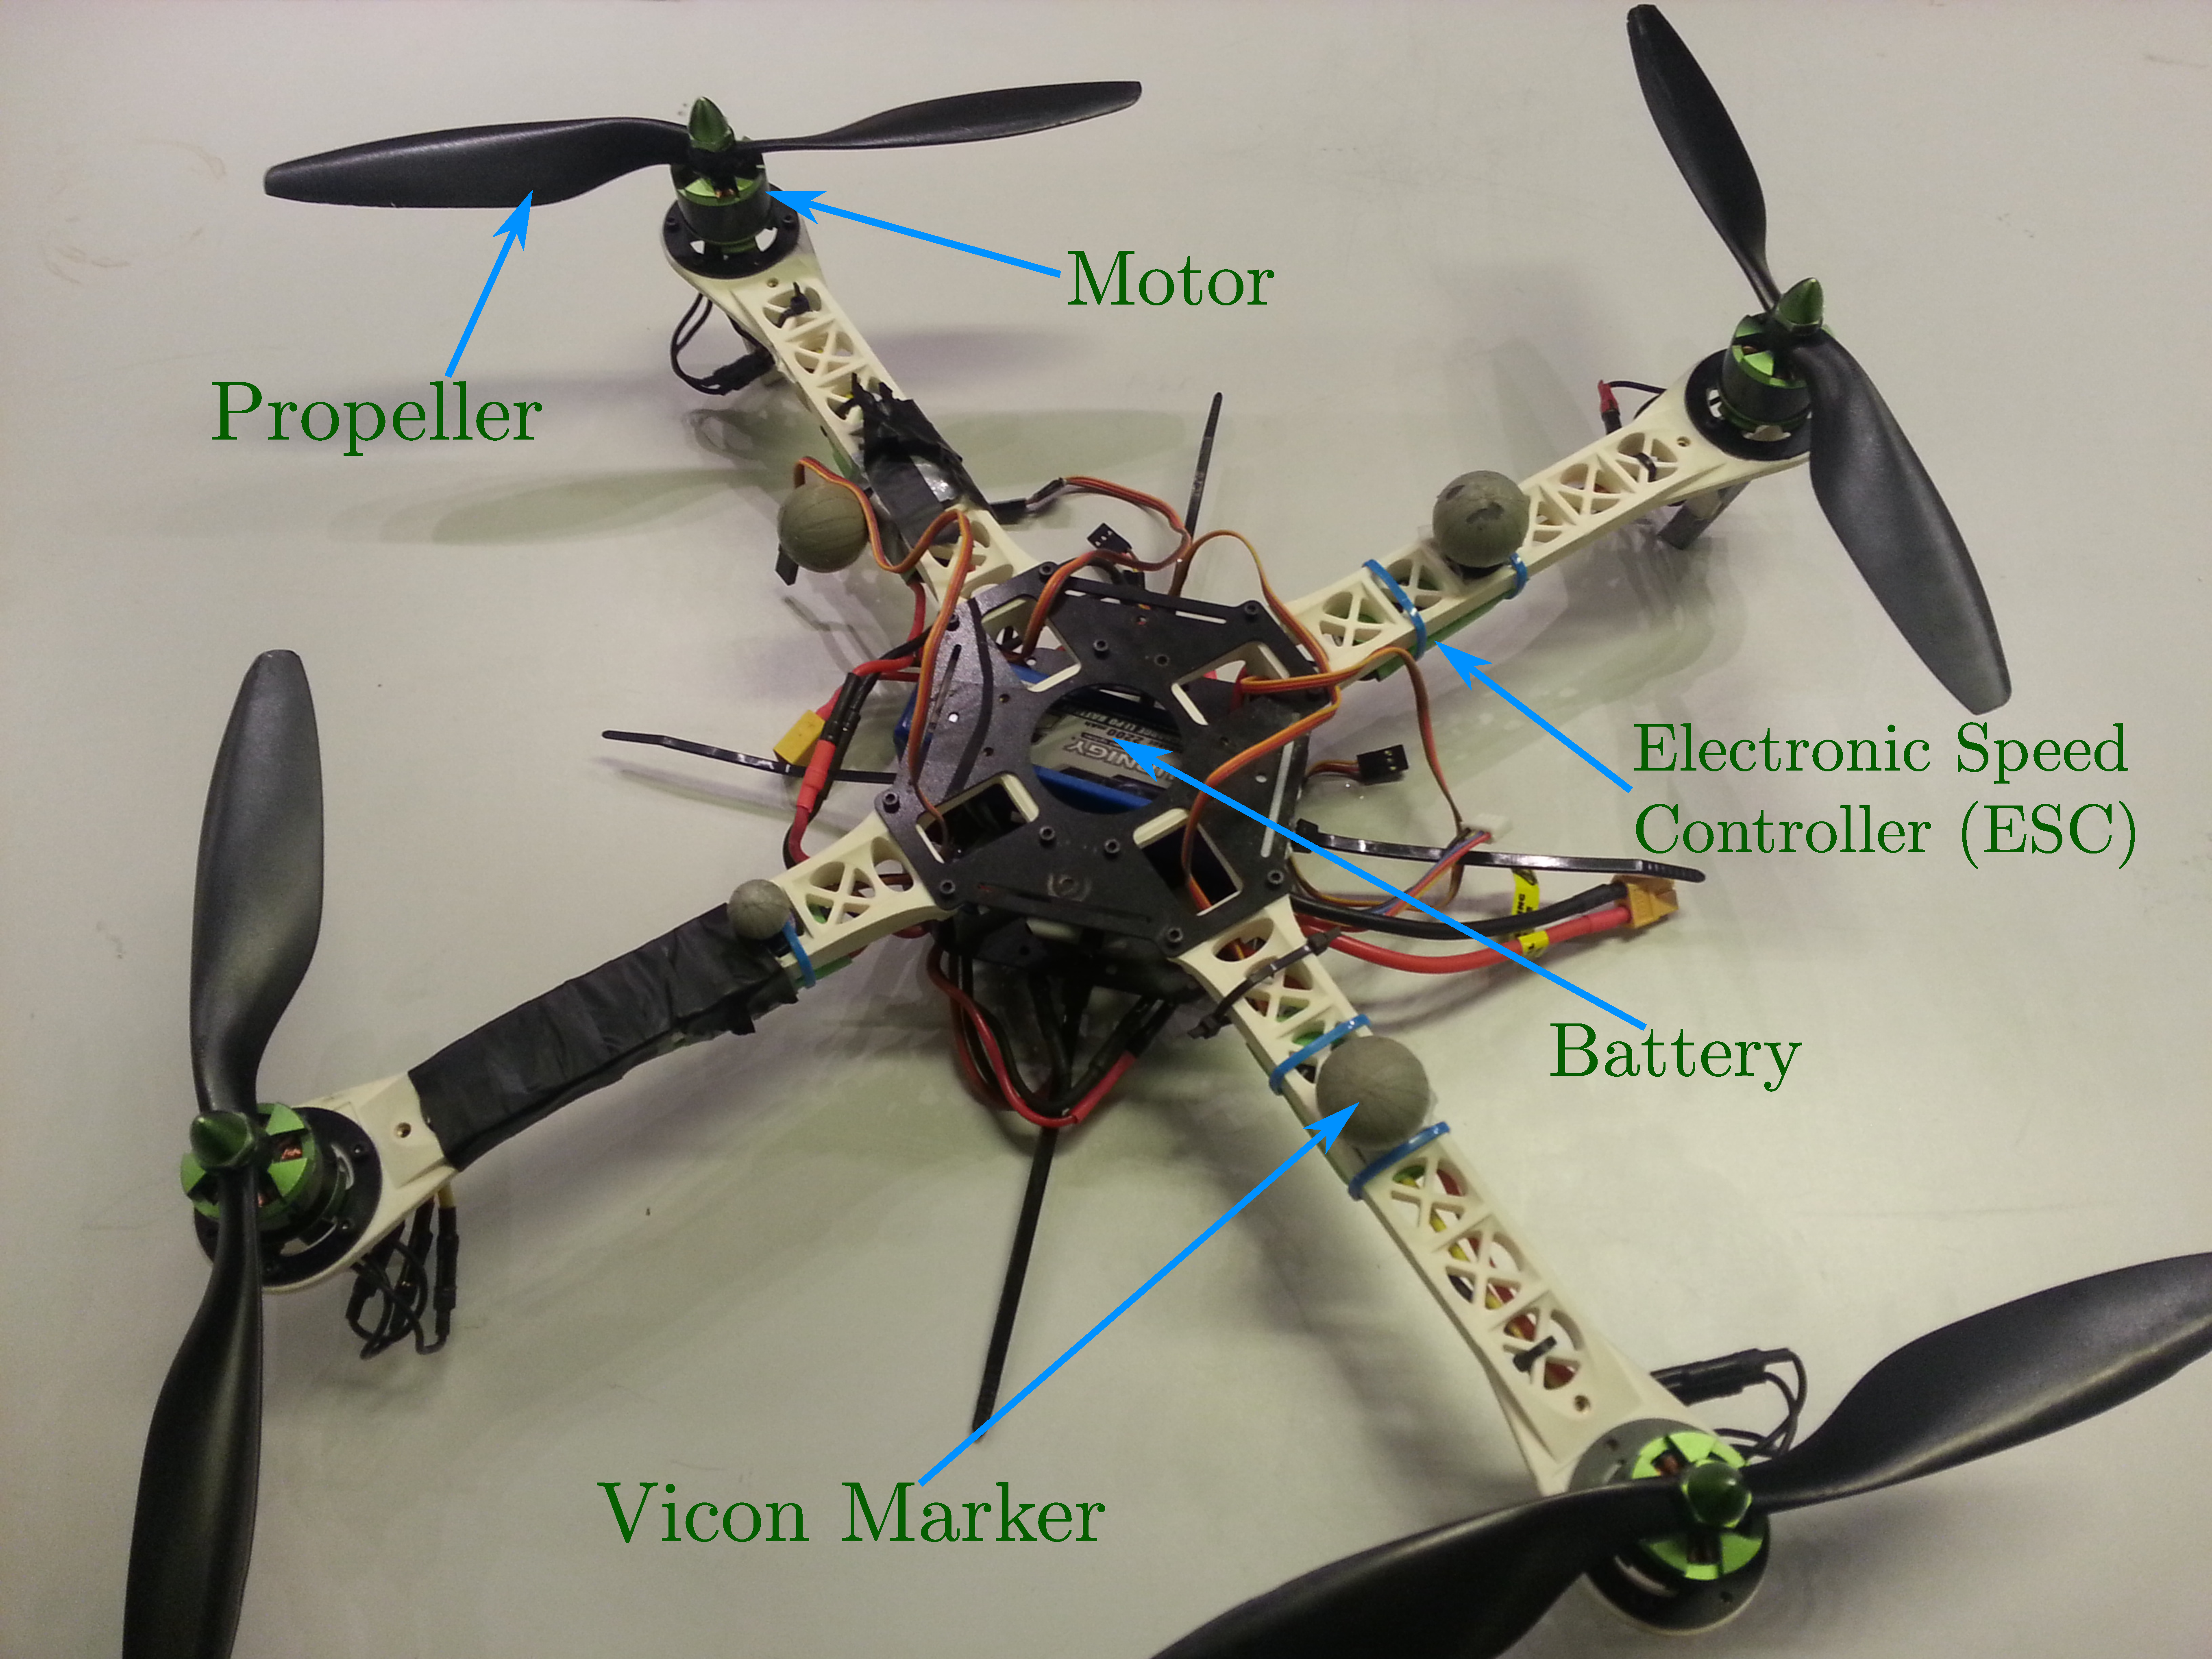
\includegraphics[width=.6\linewidth]{figures/quadcopterBaseLabels}
  \caption{The quadcopter with attached hardware as given.}
  \label{fig:systemBase}
\end{figure}
\fxnote{change figure - so vicon balls are not included.}
First the motors on the quadcopter is described.
\subsection{Motors}
The quadcopter is equipped with four brushless outrunner motors named Turnigy Multistar. 

Brushless motors are electric powered with a DC power that require a electronic commutator, which generates a sinusoidal or trapezoidal waveform, to run the motor. They have a higher power density and higher reliability than conventional DC motors.

Within this kind, outrunner motors have their magnets in the outer shell, the rotor. The rotor spins around the fixed coils that form the stator. Due to the more space in the rotor for magnets, they normally have more poles that inrunner motors, and thus, are able to produce more torque for the same size.  

The motor used has a $k_v$ of 935 $rpm/V$, 14 poles and maximum current of 15 $A$. \fxnote{Source: \url{https://www.hobbyking.com/en_us/mt2213-935kv-multistar-motor-and-propeller-combo-10x4-5-cw-ccw.html}}
\fxnote{elaborate on why this is usefull for the reader}

The motor used is shown in \autoref{fig:Motor}.
\begin{figure}[H]
	\centering
	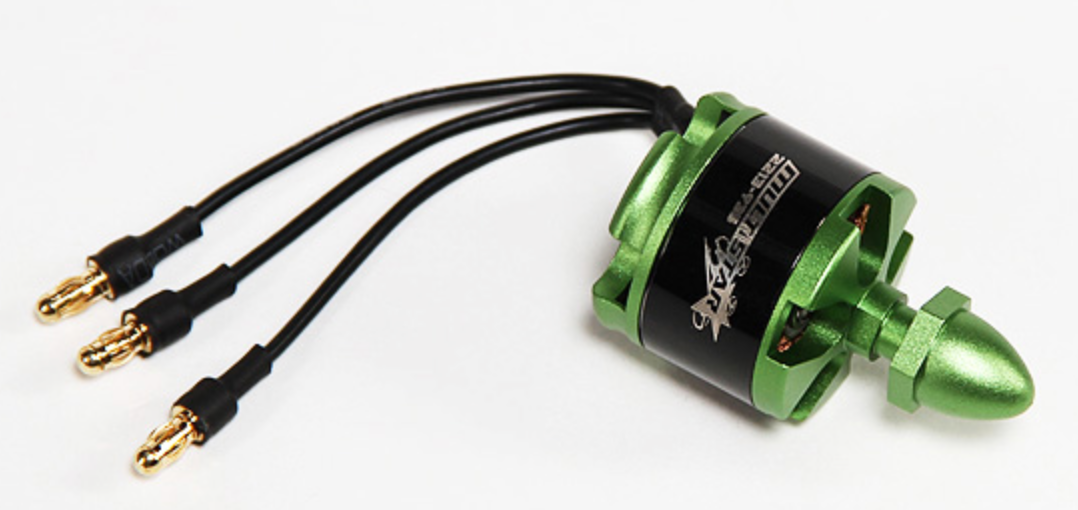
\includegraphics[scale=0.5]{figures/motor.png}
	\caption{One of the four motors mounted on the quadcopter.}
	\label{fig:Motor}
\end{figure} 


\subsection{Propellers}
The propellers are sold with the motors and are 10 inches long (25.4 cm) and has a pitch of 4.5 (11,43 cm) inches. The pitch is the distance traveled by a propeller after one complete rotation. For this to be true the propeller must turn inside a solid surface, the traveled distance is less if it rotates inside a liquid or gas. \fxnote{Source: \url{ http://www.propellerpages.com/?c=articles&f=2006-03-08_what_is_propeller_pitch}} A higher pitch creates more turbulence and make the quadcopter less steady when flying.\fxnote{Source: \url{https://oscarliang.com/quadcopter-motor-propeller/}} 

The length of the propeller is proportional to the efficiency of the quadcopter. Hence, a longer propeller has an increase in maximum speed. The acceleration of a small propeller is greater than that of a larger propeller. Thus it is easier to change the inertia of moment if utilizing a small propeller compared to a larger one. \fxnote{source: \url{https://oscarliang.com/quadcopter-motor-propeller/}} 

In this case a propeller which is 10 inches long and has a pitch of 4.5 is suitable for the utilized quadcopter, as it has been utilized in multiple cases before. 

A picture of the utilized propellers can be seen in \autoref{fig:Propeller}.

\begin{figure}[H]
	\centering
	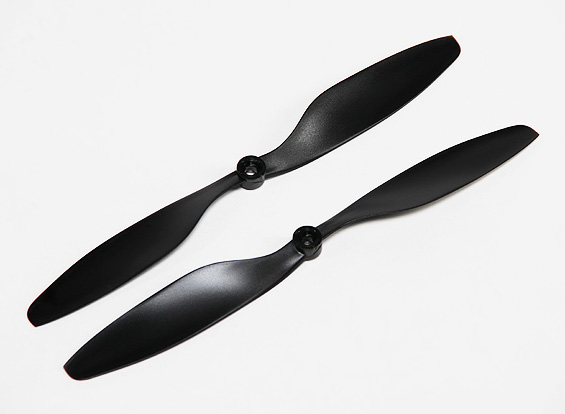
\includegraphics[scale=0.4]{figures/propeller.png}
	\caption{Two of the four propellers mounted on the quadcopter's motors.}
	\label{fig:Propeller}
\end{figure}

%The relationship between PWM signal to the motor controllers and the velocity of the propeller can be seen in Figure ZZ. \fxnote{pull diagram from measurement report}

%It has been observed during tests, that the motor runs faster as it's temperature increases. This is not expected due to the increased resistance, that occurs when the coils within the motor are heated. Therefore the relationship between PWM signal and velocity is not representative for all cases. It is however deemed reasonable to neglect this variance and presume a relationship as it is derived in the measurement report, see Appendix YY.
 
\subsection{Motor Controllers}
The quadcopter comes with four electronic speed controllers, ESCs, one for each motor. The ESCs produce an 8 kHz PWM, are rated for a 2-4 cell Li-Po battery and can handle a constant current of up to 30 A. The ESCs also has a 5.5 V, 4 A output for powering e.g. a controller board.\cite{HKing}

\begin{figure}[H]
	\centering
	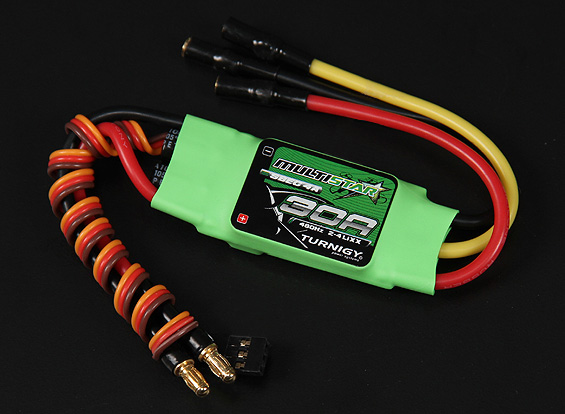
\includegraphics[scale=0.4]{figures/ESC}
	\caption{One of the four Electronic Speed Controllers mounted on the quadcopter.\cite{HKing}}
	\label{fig:esc}
\end{figure}

\subsection{Battery}
The battery available for the prototype, is a Zippy Flightmax battery. It weighs 141 gram, has a capacity of 1500 mAh, a voltage of 11.1 volts and a discharge current of 20 amperes.

%removed by Niels: It shall be noted, that the battery level...
The battery level drops over time, with a significance that can not be neglected as it may have great impact on the output of the motor and therefore on the lift of the propeller. It is possible to measure the battery level while operating the quadrotor. By taking into account the battery level in the test of the PWM signal to velocity, it is possible to obtain a quadcopter having constant lift force, if this is requested\fxnote{Niels and Alejandro suggest: With this information and knowledge of the relationship between voltage and RPM it is possible to account for the battery level, and thereby rectify the problem. [ref to test - maybe - should the test be discussed this early?]}.

\section{Selected hardware}
The provided quadcopter is simply a frame as it is not capable to fly as it is. Therefore additional hardware must be implemented in order to obtain a system that will allow the desired outcome. This includes sensors, as the quadcopter will otherwise not be able to navigate. A processor, as a computer needs to handle commands and control calculations. And lastly a wireless modules, as communication with the quadcopter is required. The chosen sensor solution is now presented.
\subsection{Sensor}
It is possible to implement on board sensors or use a real time position and attitude data capturing system called Vicon. 
As the scope of this project is to design and implement a control system, which deals with delays, it is chosen to use the Vicon system. It is ready to use and unnessary time will be spared on getting on board sensors to work. Moreover it challenges the controlsystem, as it will introduce delays of the control system. As this project develops a prototype, it is not essential, that the quadcopter can operate outside of the Vicon system.\\

The Vicon system is a powerful tool that provides real-time position and orientation data captured with 9 infrared cameras.This information can be used to track objects inside the room the system is built within.
%An example is found in Aalborg University as seen in \figref{ViconRoom}. 

%\begin{figure}[H]
%	\centering
%	\includegraphics[scale=0.5]{figures/ViconRoom}
%	\caption{Aalborg University's Vicon room.}
%	\label{ViconRoom}
%\end{figure}

To use this system, markers are attached to the object that is to be tracked. The Vicon system streams the position of the markers and the position and orientation of the object at 100 Hz for a computer to read them. The data can be received by using an SDK plugin for MATLAB. In this way, data can be operated in the MATLAB environment, making it easier to obtain variable derivatives like velocities or accelerations.

The user interface of the Vicon system is shown in \autoref{fig:ViconTracker}. 
\begin{figure}[H]
	\centering
	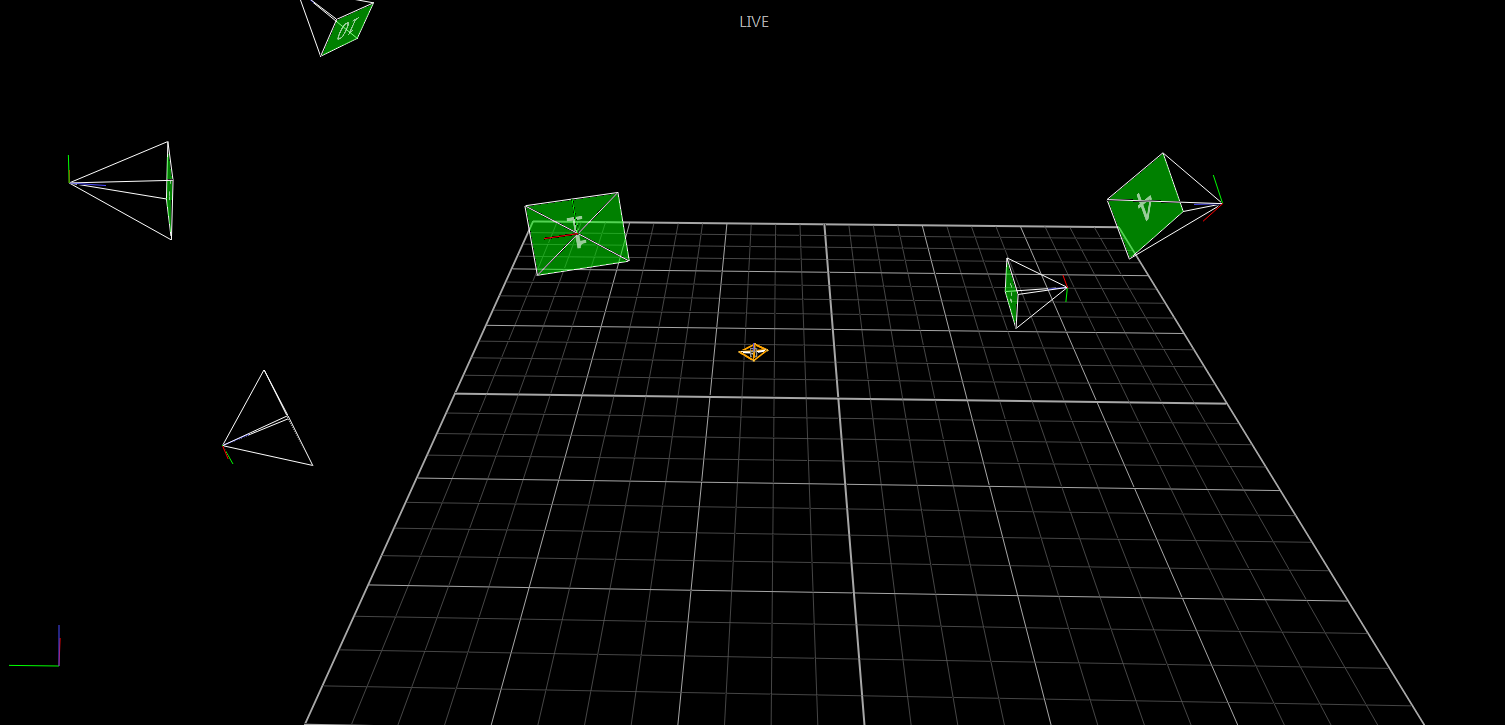
\includegraphics[scale=0.27]{figures/ViconTracker}
	\caption{User interface of the Vicon System, the Vicon Tracker. An object has been created from the markers placed on the drone.}
	\label{fig:ViconTracker}
\end{figure}
It is called Vicon Tracker and it allows the creation of objects by grouping markers present in the room. It also allows to change the center of gravity of the created objects and rotate the inertial and body reference frames to any desired orientation.


\subsection{Processor}
As the computer on the ground is only to handle the Vicon sensor data and the communication of this data, the processor of the quadcopter must be capable of handeling the processing of the controlsystem along with recieving the position and attitude date of the quadcopter.
The implementation of the controllers is done in a microprocessor from Atmel, the ATmega2560, mounted in the ArduinoMEGA development board, as seen in figure \autoref{fig:ATmega}. This is deemed strong enough to handle the required dataload and fast enough to not obscure the control of the quadcopter. \fxnote{language, and we dont provide any info on these assumptions}

This processor has up to 16 PWM output channels, two 8-bit timers and four 16-bit timers, four USART modules, 8 kilobytes of internal memory and a processing speed of 16 MIPS. With this capabilities, a quadcopter control could be implemented.

The use of the development board makes the use of the wireless modules easier as an arduino shield can be directly plugged in. Furthermore, it allows a faster set up of the microcontroller as all required hardware (oscillatior, power supply, etc.) is already present in the board. 
\begin{figure}[H]
	\centering
	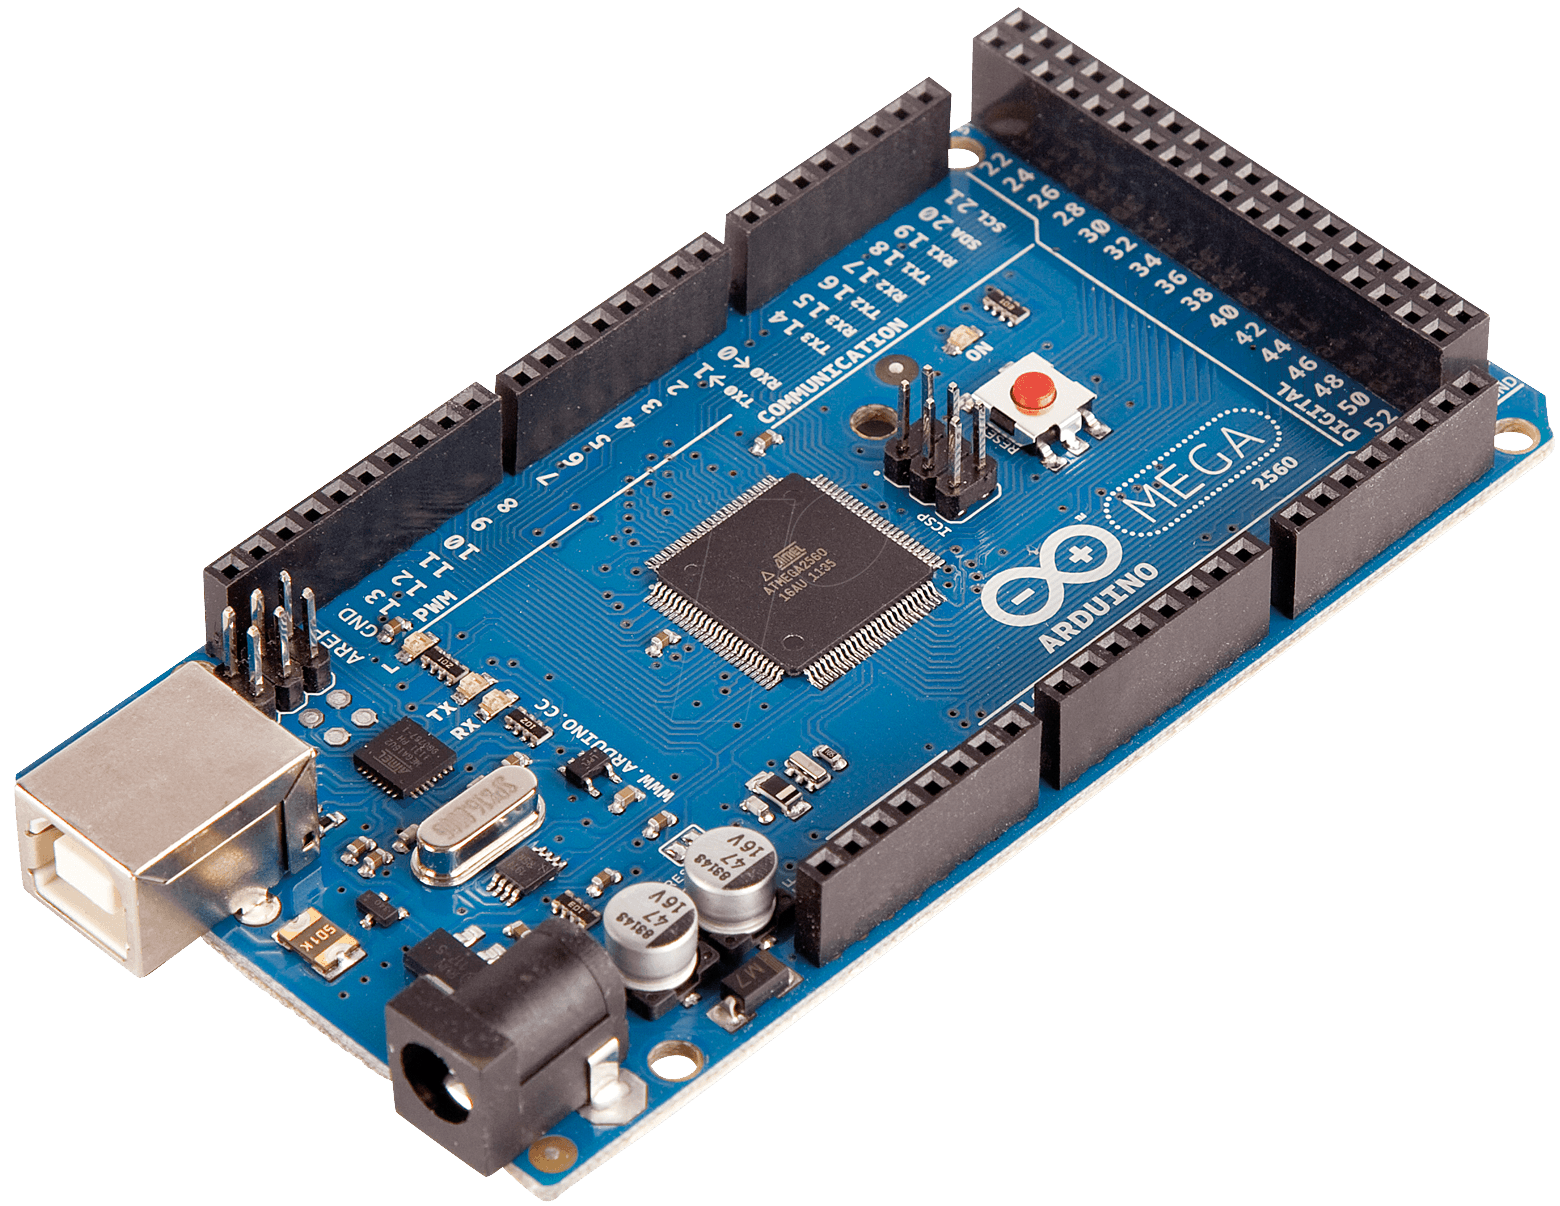
\includegraphics[scale=0.17]{figures/ARDUINO_MEGA}
	\caption{AtMega2560 mounted in the ArduinoMEGA development board.}
	\label{fig:ATmega}
\end{figure}
\subsection{Wireless Modules}

The wireless modules used to communicate with the quadcopter are called XBee, see \autoref{fig:XBEE}. They communicate at a 2.4 GHz frequency and they take care of all communication layers but the transport layer protocol. In order to use this modules, the packet has to be sent through the serial port when using the computer or through the USART module when using the microcontroller.  \fxnote{USART? UART perhaps?}
\begin{figure}[H]
	\centering
	\includegraphics[scale=0.4]{figures/XBEE}
	\caption{XBee wireless modules.}
	\label{fig:XBEE}
\end{figure}

As the provided hardware and the selected hardware have now been presented a system description is now following. 		
	\section{Prototype Description}
In the following section an overall description of the prototype is given. This is done to help the reader understand the utilized setup in the project.
The prototype is divided into 3 separate subsystems. The quadcopter, the ground station, and the vicon system. These can be seen in \figref{prototypediagram}. 

\begin{figure}[H] 
	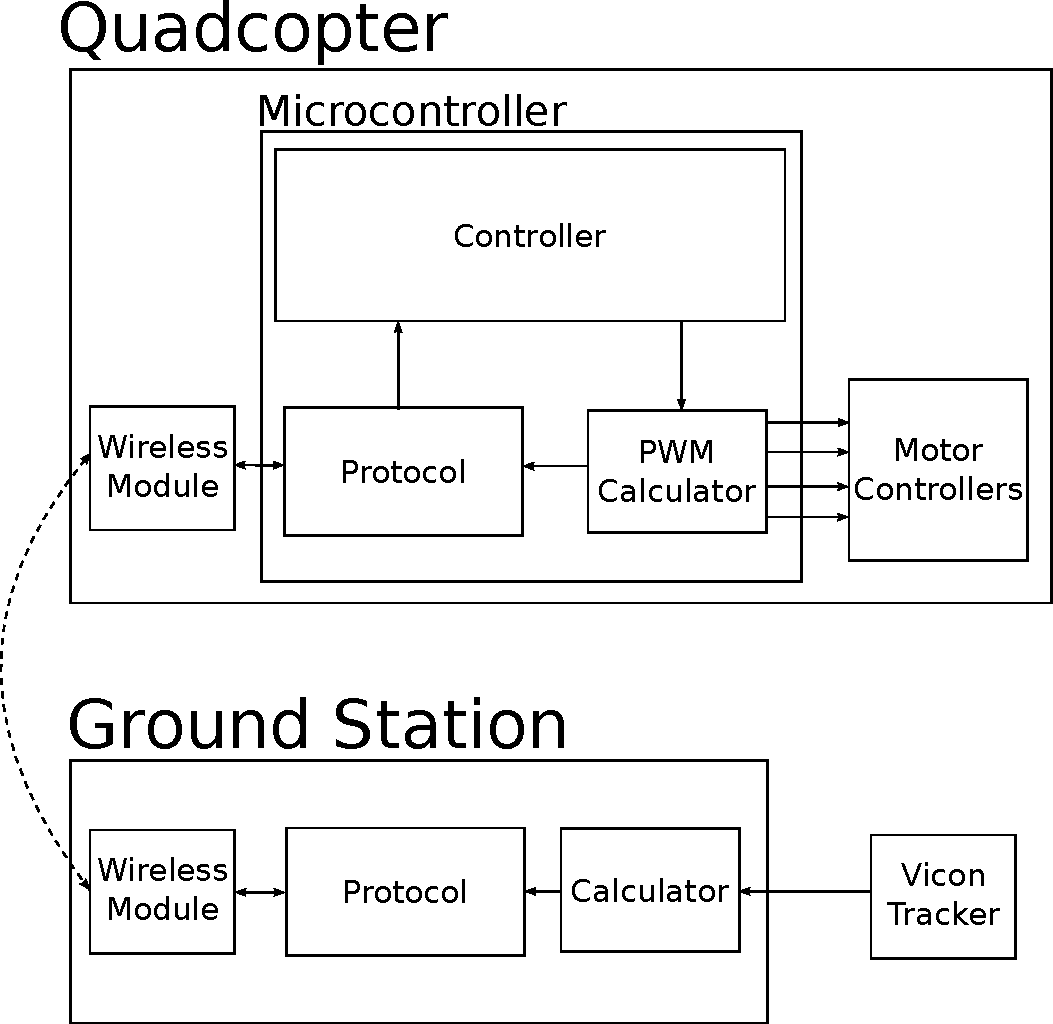
\includegraphics[scale=.5]{figures/prototypediagram}
	\centering
	\captionsetup{justification=centering}
	\captionof{figure}{Schematic diagram of the prototype, which includes the quadcopter, the ground station and the vicon system.}
	\label{prototypediagram}
\end{figure}

%!!explain somewhere what vicon is and that it can be found in aalborg university, maybe we should have a little section, together with all the other hardware?!!

For this project the Vicon system is used to capture the position and orientation of the quadcopter. This avoids the time consuming sensor set up on the quadcopter, as the Vicon system is already configured and ready to use. The Vicon system is described in further detail in section ??. The Vicon system captures the quadcopters position, in form of coordinates, and its orientation, in the form of euler angles. The information is then transmitted to the Ground Station.

The Ground Station utilizes the data it receives from the Vicon system to calculate the linear velocity and linear acceleration of the quadcopter. References commands for controller, located on the quadcopter, are also needed and are generated from the ground station. These are transmitted together with the position, orientation, linear velocity and linear acceleration to the quadcopter. This information is transmitted by means of a generated network interface and a wireless module.

The quadcopter consist of a microcontroller, four motor controllers, four motors, a battery, and a wireless module. The microcontroller main tasks is to handle the network between itself and the ground station, the control calculations and to generate the control signals which should be transmitted to the four motorcontrollers. \\To be able to calculate the rotational speed needed for the motors, the five variables received from the ground station are needed, i.e the control reference, position, orientation, linear velocity and linear acceleration of the quadcopter. Hereafter it is possible to calculate the necessary PWM signals, by utilizing the rotational speed calculated by the controller and the measured voltage on the battery. \\Furthermore, the quadcopter should be able to send the battery voltage level to the ground station in order to detect when the flight should end.

%The quadcopter's most complex component is the microcontroller. It handles the control calculations, the PWM calculations according to the required control action and battery level, and the communication protocol necessary to exchange data with the ground station.

%The microcontroller requires 4 PWM outputs with different and independent duty cycles for controlling the 4 motors in the quadcopter. 

%The network interface in the microcontroller handles the incoming data from the ground station. This data consist of reference commands for the controllers and sensor data. It should also be able to send the battery voltage level to the ground station in order to detect when to end the flight.

%The communication between the ground station and the quadcopter is done through wireless modules. These should allow the implementation of the communication by designing only the transport layer protocol.

%The ground station gathers the information coming from the Vicon system and sends it to the quadcopter. This also includes doing calculations with the received Vicon data to obtain other variables like velocities or accelerations.

%Finally, Vicon system uses the position of the markers placed in the quadcopter to provide its position and orientation. The orientation data is given in multiple forms but only Euler angles data is considered.


%\textbf{Battery should be moved somewhere else}
%The battery, which is available for the prototype, is a Zippy Flightmax battery. Its weights 141 gram, has an capacity of 1500 mAh, a voltage of 11.1 volts and a discharge current of 20 amperes. 





	%---------- Chapter 3 ----------------------------------------

	%---------- Chapter 4 ---------------------------------------- 
	\chapter{Model}
To make the quadcopter have a steady flight mode it is convenient to derive a model of the system, that describes its physical behaviour. From this, a control system must be designed such that the desired flying characteristics are obtained. 
This chapter presents the model. 

First, a model overview is presented. Then, the model derivation and lastly, the model is linearized as this is necessary to be able to design a linear control system. The model and the linearized model are compared in simulations. This ensures that the linear model is an acceptable approximation.

\section{Model overview}
The model can be split into two sub models. One being an angular model describing how the angles change according to the action of the propellers and how they influence each other. The other sub model is a translational velocity model, that describes the angles, the positions and the velocities in the directions of the x-, y- and z-axes. 
These models will later be combined. 
\begin{figure}[H]
\centering
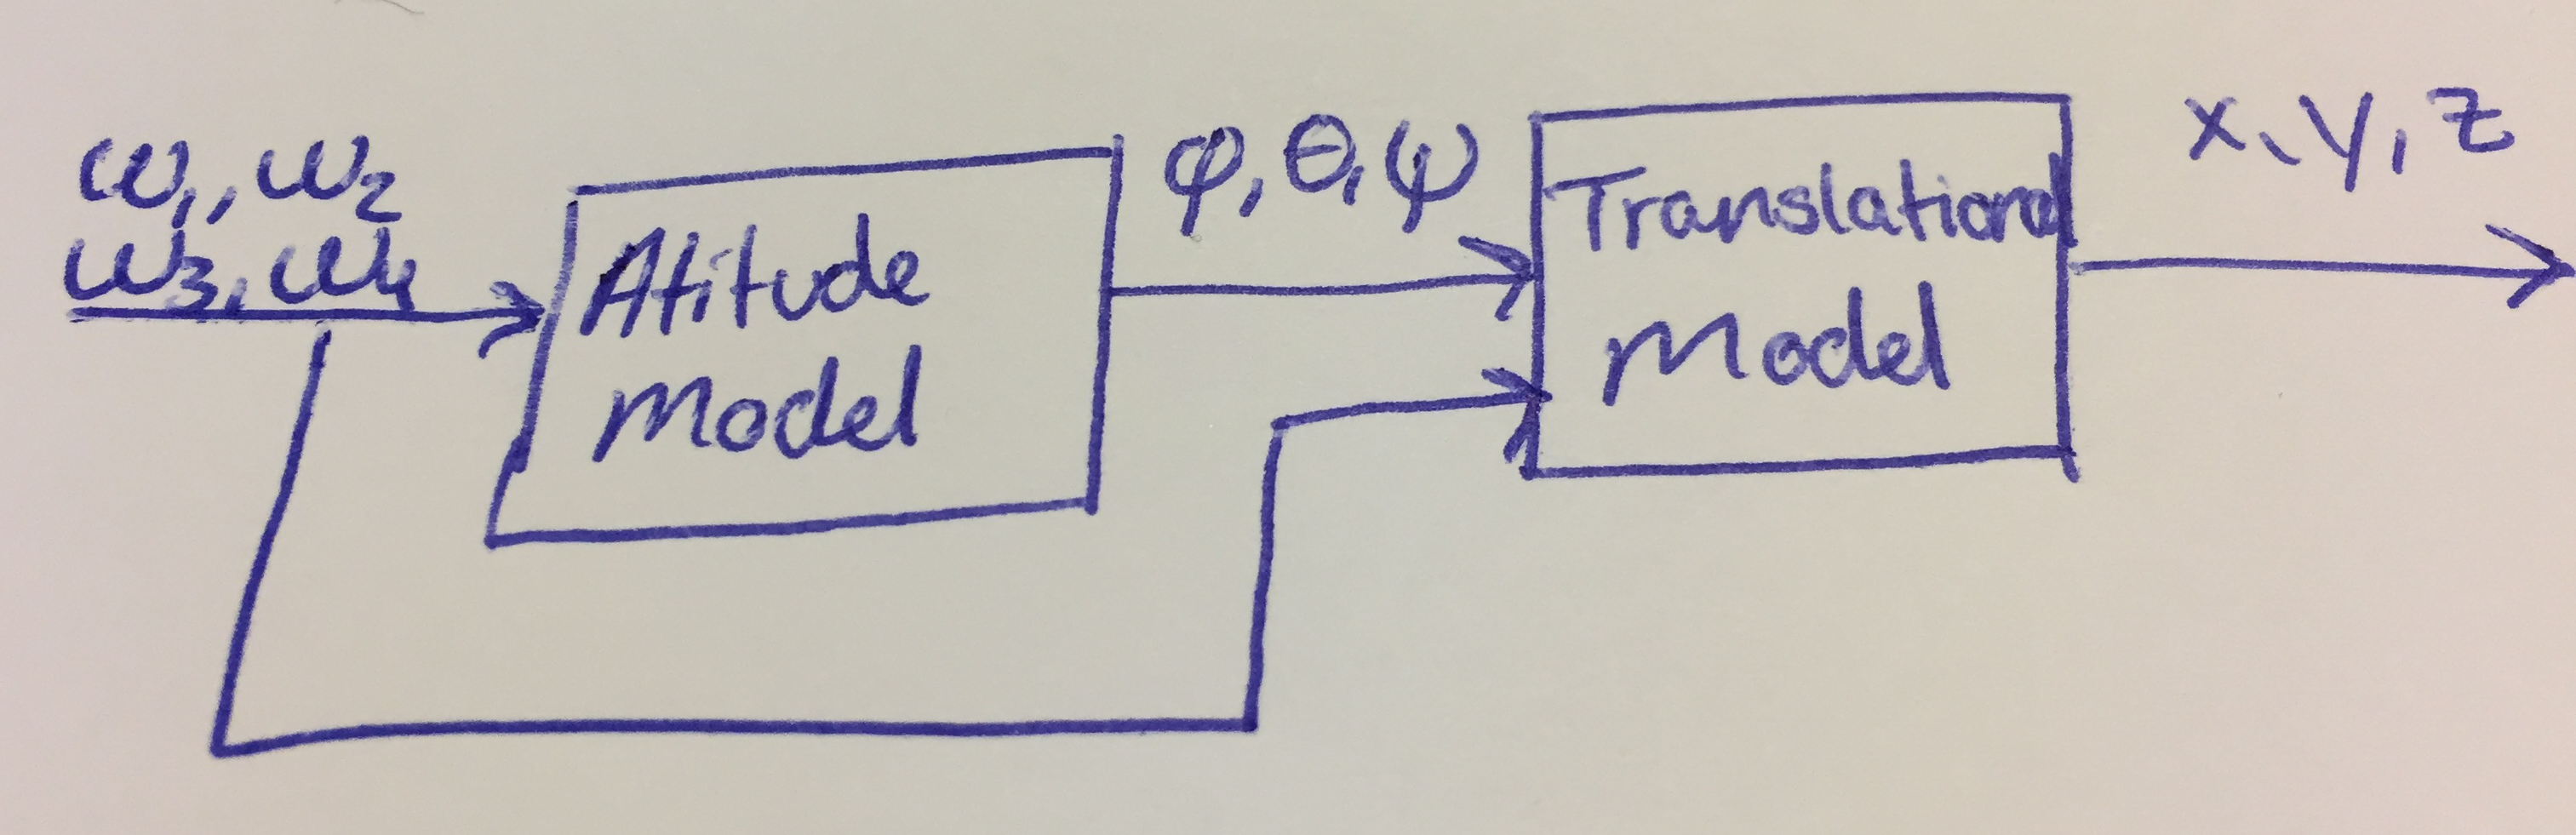
\includegraphics[scale=0.1]{figures/modeloverview.PNG}
\caption{Overview of how the model is split.}
\label{sss}
\end{figure}
When modeling the quadcopter, two coordinate systems are used. A body frame, that is fixed to the flying object and an inertial frame, that is fixed as the Vicon room. 

It is necessary to use both, as it is desired to know where the quadcopter is within the inertial frame to determine its position. To obtain the orientation of the quadcopter, the body frame's orientation compared to the inertial frame yields the angles of roll, pitch and yaw. 
%Angle and Linear
%Explain the two frames and include drawing showing them
%Flow of the chapter

%\Figref{diagramQuad} shows a representation of the quadcopter where two reference systems, inertial and body, can be seen, as well as the conventions for angles of rotation and forces. \Figref{diagramTorque} shows the body from above and includes the chosen convention for the torques produced by the propellers.
%
%\begin{minipage}{\linewidth}
%	\begin{minipage}{0.45\linewidth}
%		\begin{figure}[H]
%			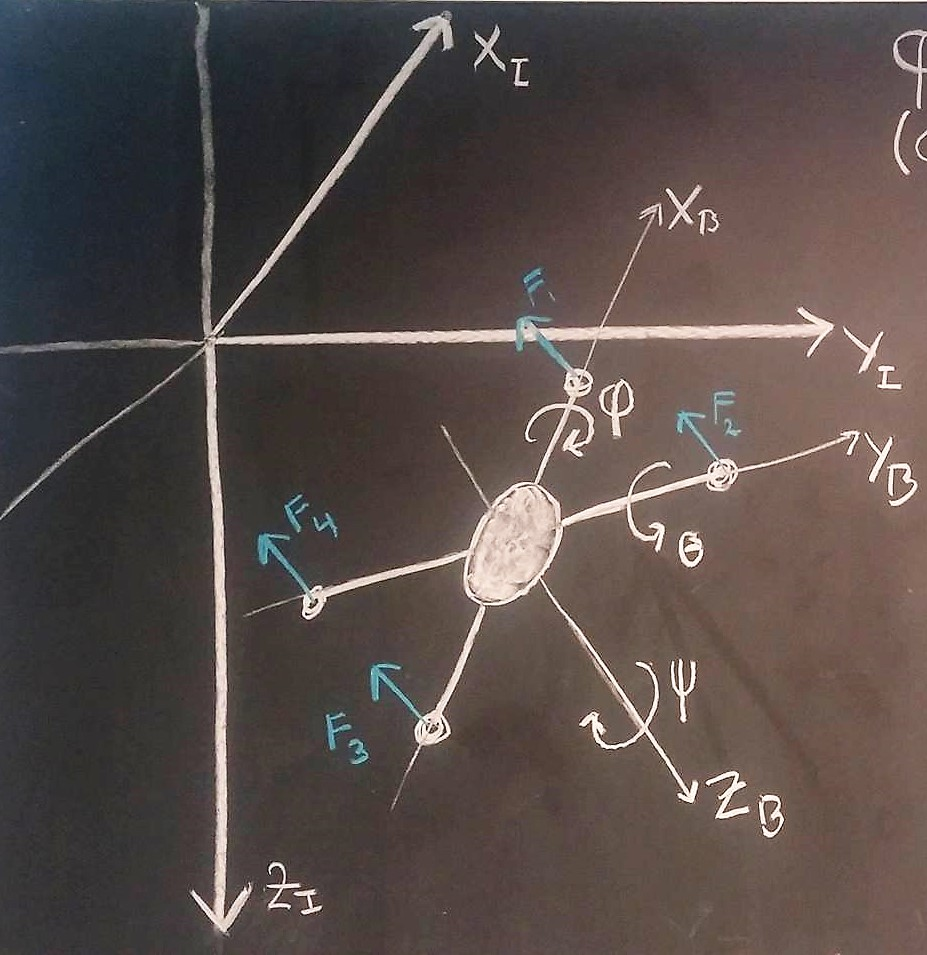
\includegraphics[scale=.27]{figures/drone_diagram}
%			\centering
%			\captionsetup{justification=centering}
%			\captionof{figure}{Diagram of the quadcopter which includes inertial and body reference systems, as well as the references for the angles (roll, pitch and yaw) and the thrust forces produced by the propeller. }
%			\label{diagramQuad}
%		\end{figure}
%	\end{minipage}
%	\hspace{0.03\linewidth}
%	\begin{minipage}{0.45\linewidth}
%		\begin{figure}[H] \vspace{16mm}
%			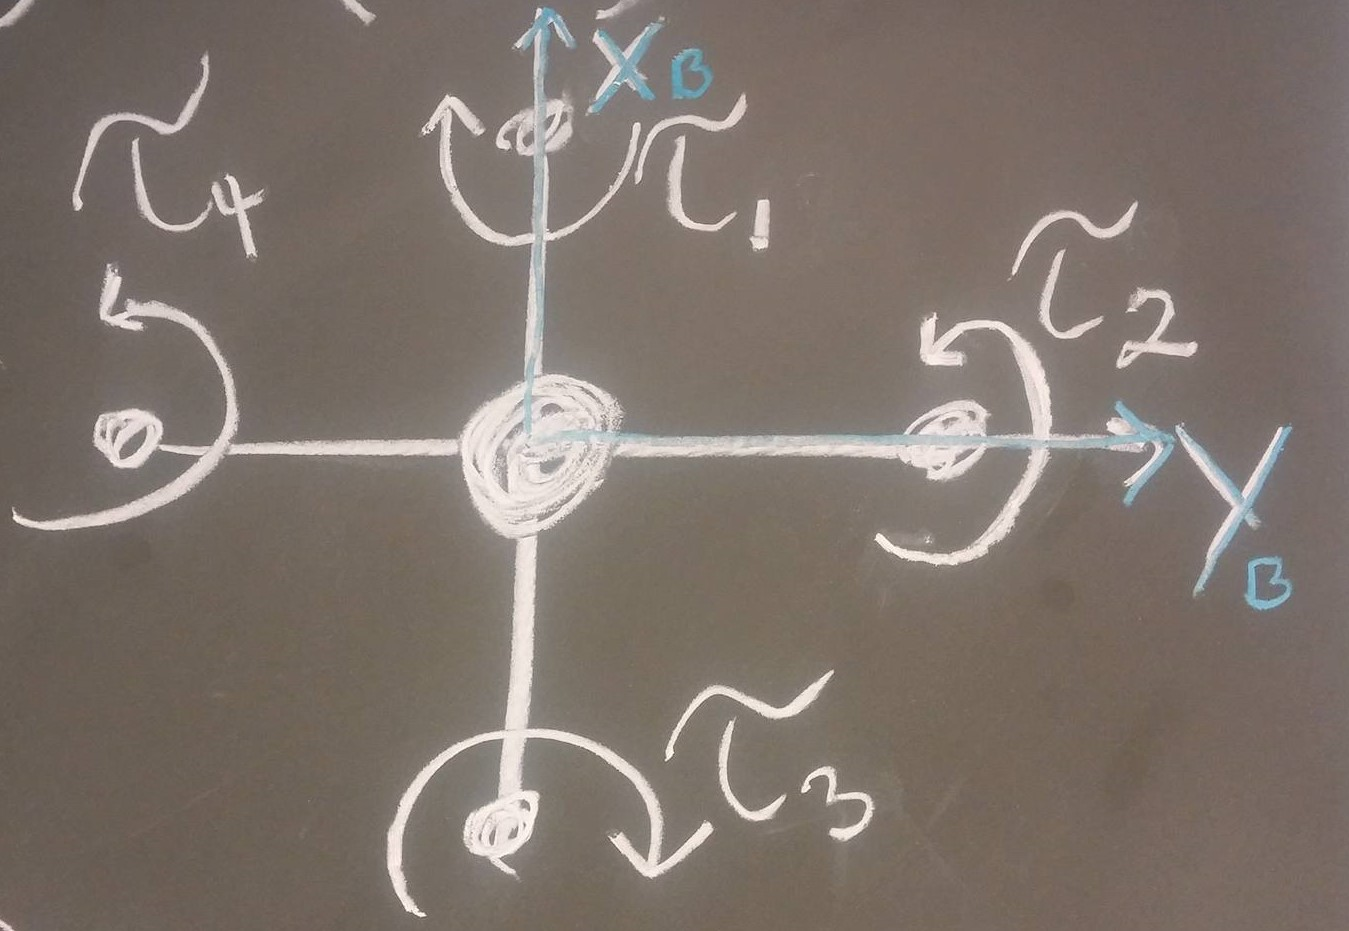
\includegraphics[scale=.18]{figures/torques_diagram}
%			\centering
%			\captionsetup{justification=centering}
%			\captionof{figure}{Diagram of the quadcopter from above, with the references for the torques produced by the drag force at the propeller.}
%			\label{diagramTorque}
%		\end{figure}
%	\end{minipage}
%\end{minipage}
In the following section the attitude model is derived. 
	\section{Attitude Model} \label{sec:AttitudeModel}
The attitude model of the quadcopter describes how the roll, pitch and yaw angles evolve according to the forces and torques exerted by the propellers. 

The basis for deriving the model are the free body diagrams illustrated in \autoref{fig:droneDiagram} and \ref{fig:torquesDiagram}. 

\begin{minipage}{\linewidth}
	\begin{minipage}{0.6\linewidth}
		\begin{figure}[H]
			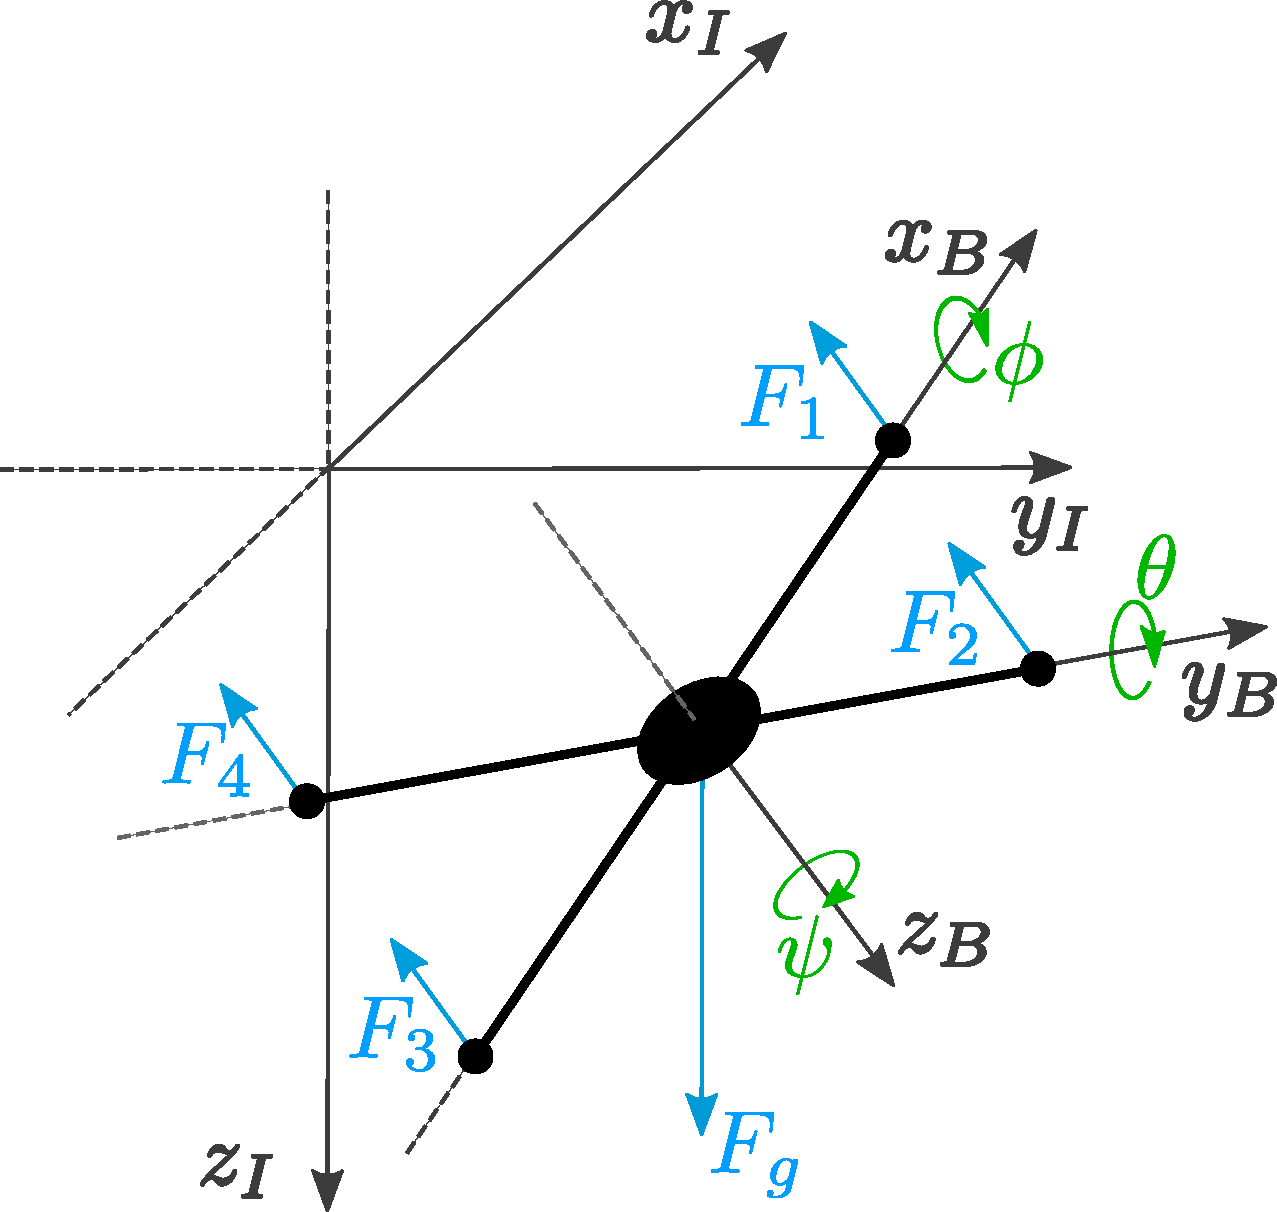
\includegraphics[scale=.4]{figures/droneDiagram}
			\centering
			
			\captionof{figure}{Free body diagram that holds both the inertial and body reference systems, as well as the references for the angles, roll, pitch and yaw.}
			\label{fig:droneDiagram}
		\end{figure}
	\end{minipage}
	\hspace{0.03\linewidth}
	\begin{minipage}{0.35\linewidth}
		\begin{figure}[H] \vspace{20mm}
			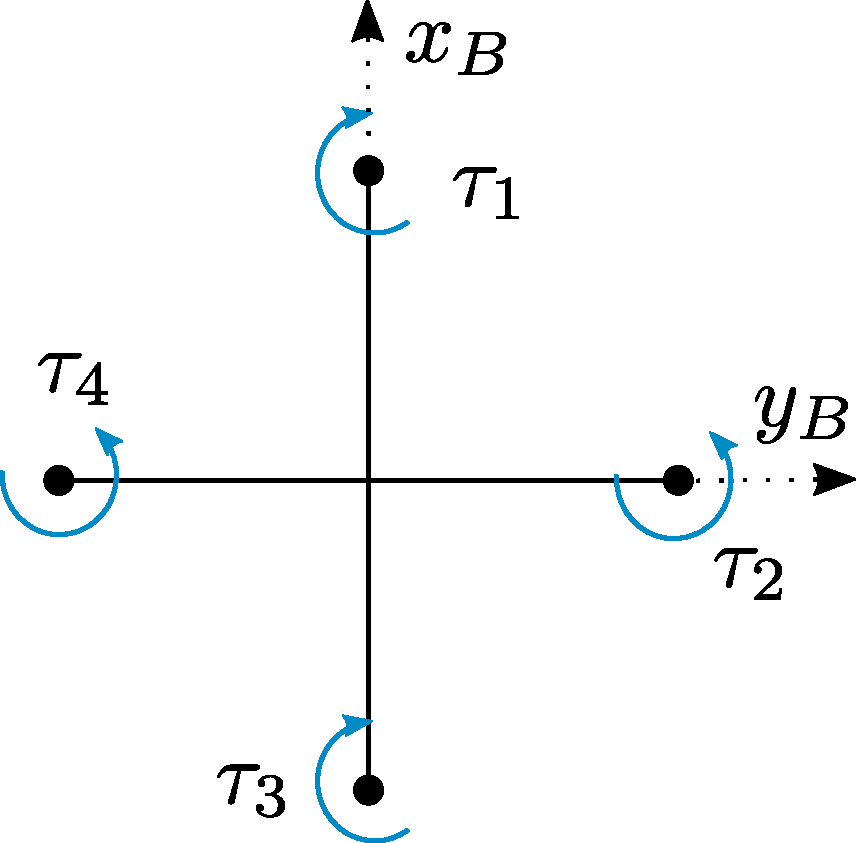
\includegraphics[scale=.4]{figures/torquesDiagram}
			\centering
            \vspace{10mm}
			\captionof{figure}{Free body diagram with the references for the torques produced by the drag forces at the propellers.}
			\label{fig:torquesDiagram}
		\end{figure}
	\end{minipage}
\end{minipage}

From the diagrams above, the equations of angular motion along the three body axes can be derived by first principles modeling, that is, using only laws of physics. In this case, Newton's Second Law for rotational motion, as seen in \autoref{eq:newtonangular}.
%
\begin{align}
	J\cdot\alpha=\sum\tau
	\label{eq:newtonangular}
\end{align}
\begin{where}
\va{J}{is the moment of inertia}{kg \cdot m^2}
\va{\alpha}{is the angular acceleration}{rad\cdot s^{-2}}
\va{\tau}{are the torques applied to the system}{N \cdot m}
\end{where}

%\begin{where}
%	\va{J}{is the moment of inertia}{kg\cdot m^2}
%	\va{\alpha}{is the angular acceleration}{rad\cdot m\cdot s^{-2}}
%	\va{\tau_i}{are the torques applied to the system}{Nm}
%\end{where}
%It shall be noted, that the fact that Newton's laws, that only apply in relation to an inertial reference, are applied even though the earth is accelerating and rotating, as it is the assumption, that it is of little influence for the system of the quadcopter. 
%
From applying Newton's Second Law, \autoref{eq:AngleEq1}, \ref{eq:AngleEq2} and \ref{eq:AngleEq3} are obtained. As it can be seen, the roll and pitch angular accelerations depend on the thrust forces exerted by the propellers placed along the y- and x-axis of the quadcopter, respectively. The yaw angle changes due to the torques created by the drag forces in the propellers.
%
\begin{align}
	J_x\cdot\ddot{\phi}&=(F_4-F_2)\cdot L  \label{eq:AngleEq1} \\
	J_y\cdot\ddot{\theta}&=(F_1-F_3)\cdot L  \label{eq:AngleEq2}\\
	J_z\cdot\ddot{\psi}&=\tau_1-\tau_2+\tau_3-\tau_4
	\label{eq:AngleEq3}
\end{align}
\begin{where}
\va{J_x}{is the inertia around the x axis}{kg\cdot m^2}
\va{J_y}{is the inertia around the y axis}{kg\cdot m^2}
\va{J_z}{is the inertia around the z axis}{kg\cdot m^2}
\va{\ddot{\phi}}{is the roll angular acceleration}{rad\cdot s^{-2}}
\va{\ddot{\theta}}{is the pitch angular acceleration}{rad\cdot s^{-2}}
\va{\ddot{\psi}}{is the yaw angular acceleration}{rad\cdot s^{-2}}
\va{F_i}{is the thrust force from each propeller}{N}
\va{L}{is the length from center of mass to motor}{m}
\va{\tau_i}{is the drag torque from each propeller}{N \cdot m}
\end{where}

%\begin{where}
%\va{\ddot{\phi}}{is roll angular acceleration}{rad $\cdot$ s$^{-2}$}
%\va{\ddot{\theta}}{is  pitch angular acceleration}{rad$\cdot$ s$^{-2}$}
%\va{\ddot{\psi}}{is yaw angular acceleration}{rad$\cdot$ s$^{-2}$}
%\va{J_x}{is the body moment of inertia around $x_B$ direction}{kg $\cdot$ m$^2$}
%\va{J_y}{is the body moment of inertia around $y_B$ direction}{kg $\cdot$ m$^2$}
%\va{J_z}{is the body moment of inertia around $z_B$ direction}{kg $\cdot$ m$^2$}
%\va{L}{is the length of the arm of the quadcopter}{m}
%\va{F_n}{is the thrust force produced in each propeller}{N}
%\va{\tau_n}{is the torque due to the drag force in each propeller}{Nm}
%\end{where}
The thrust forces and drag torques from the propeller can be assumed to be proportional to the square of the velocity of the motor, related by constants obtained as described in \autoref{app:ThrustTest} and \ref{app:TorqueTest}. The equations above can be rewritten to include these terms.
%
\begin{align}
J_x\cdot\ddot{\phi}&=k_{th} \cdot(\omega^2_4-\omega^2_2) \cdot L \label{eq:AngleEqVelocities1}\\
J_y \cdot\ddot{\theta}&=k_{th} \cdot(\omega^2_1-\omega^2_3) \cdot L \label{eq:AngleEqVelocities2} \\
J_z\cdot\ddot{\psi}&=k_d \cdot(\omega^2_1-\omega^2_2+\omega^2_3-\omega^2_4)
\label{eq:AngleEqVelocities3}
\end{align}
\begin{where}
\va{k_{th}}{is the thrust constant}{N\cdot s^2 \cdot rad^{-2}}
\va{k_d}{is the drag constant}{N \cdot m\cdot s^2 \cdot rad^{-2}}
\end{where}

\autoref{eq:AngleEqVelocities1}, \ref{eq:AccelerationEqInertialVelocities2} 
and \ref{eq:AccelerationEqInertialVelocities3} are the final attitude model expressions that are brought forward. %Now that the attitude model is known, the translational model must be derived. This is done in the following section. 
	\section{Translational Model} \label{sec:TranslationalModel}
The aim of this section is to model the translational behavior of the quadcopter. This can be done from \autoref{fig:droneDiagram} in \autoref{sec:AttitudeModel}. An equation for translational accelerations of each specific axis in the inertial frame can be derived by using Newton's Second Law.
%
\begin{flalign}
    m a = \sum F
\end{flalign}
%
\begin{where}
\va{m}{is the mass}{kg}
\va{a}{is the translational acceleration specific for each axis in the inertial frame}{m \   s^{-2}}
\va{F}{are the forces applied to the system}{N}
\end{where}

All the forces that are applied to the quadcopter create an acceleration on it. The forces are the thrust, which the propellers generate, and the gravitational force.

As seen in \autoref{fig:droneDiagram} in \autoref{sec:AttitudeModel} the gravitational force has effect only in the $z_{\mathrm{I}}$ direction and the four forces from the motors need to be transformed into the inertial system. This is done through the rotation matrix showed in \autoref{eq:RotMatrix}.
\fxnote{Anders: Hmmm, you need more details on how you do this? How do you use the 3x3 rotation matrix to obtain (3.10)-(3.12)?}

Taking into account this transformation, the movement can be described using \autoref{eq:AccelerationEqInertial1}, \ref{eq:AccelerationEqInertial2} and \ref{eq:AccelerationEqInertial3}.
%
\begin{flalign}
    m \ddot{x}_{\mathrm{I}} &= -(F1+F2+F3+F4) (\cos\phi \sin\theta \cos\psi + \sin\phi \sin\psi)  \label{eq:AccelerationEqInertial1}\\
    m \ddot{y}_{\mathrm{I}} &= -(F1+F2+F3+F4) (\cos\phi \sin\theta \sin\psi - \sin\phi \cos\psi)   \label{eq:AccelerationEqInertial2}\\
    m \ddot{z}_{\mathrm{I}} &= F_g-(F1+F2+F3+F4) \cos\phi \cos\theta
    \label{eq:AccelerationEqInertial3}
\end{flalign}
%
\begin{where}
    \va{\ddot{x}_{\mathrm{I}}} {is the translational acceleration in the $x_{\mathrm{I}}$ direction}        {m \  s^{-2} }
    \va{\ddot{y}_{\mathrm{I}}} {is the translational acceleration in the $y_{\mathrm{I}}$ direction}        {m \  s^{-2} }
    \va{\ddot{z}_{\mathrm{I}}} {is the translational acceleration in the $z_{\mathrm{I}}$ direction}        {m \  s^{-2} }
    \va{F_g} {is the gravitational force acting on the quadcopter} {N}
\end{where}

These equations can also be rewritten taking into account that the forces are assumed to be proportional to the square of the speeds of the motors. This assumption results in \autoref{eq:AccelerationEqInertialVelocities1}, \ref{eq:AccelerationEqInertialVelocities2} and \ref{eq:AccelerationEqInertialVelocities3}.
%
\begin{flalign}
    m \ddot{x}_{\mathrm{I}} &= -k_{\mathrm{th}} ({\omega_1}^2+{\omega_2}^2+{\omega_3}^2+{\omega_4}^2) (\cos\phi \sin\theta \cos\psi + \sin\phi \sin\psi)   \label{eq:AccelerationEqInertialVelocities1}\\
    m \ddot{y}_{\mathrm{I}} &= -k_{\mathrm{th}} ({\omega_1}^2+{\omega_2}^2+{\omega_3}^2+{\omega_4}^2) (\cos\phi \sin\theta \sin\psi - \sin\phi \cos\psi)  \label{eq:AccelerationEqInertialVelocities2}\\
    m \ddot{z}_{\mathrm{I}} &= F_g-k_{\mathrm{th}} ({\omega_1}^2+{\omega_2}^2+{\omega_3}^2+{\omega_4}^2) \cos\phi \cos\theta
    \label{eq:AccelerationEqInertialVelocities3}
\end{flalign}
%
\autoref{eq:AccelerationEqInertialVelocities1}, \ref{eq:AccelerationEqInertialVelocities2} and \ref{eq:AccelerationEqInertialVelocities3} are the final model expressions of the translational model.

Now that both the attitude model and the translational model are derived, it is desirable to linearise the model expressions. 
	\section{Linearization} \label{sec:Linearization}
%Compare to non linear (simulation)\\
%Since the goal is to design a linear controller, it is necessary to linearize the equations
%around an equilibrium point. The attitude equations in the body frame,
%1 , must be lin-
%earized since they contain squared velocities. The translational equations in the inertial
%frame, Equation 3.10, 3.11, and 3.12, must also be linearized since these contain trigono-
%metric functions and squared velocities. The equilibrium point is chosen to be where the
%quadcopter is hovering at a fixed position in the inertial frame. This happens when roll
%and pitch are kept to zero. The forces along the x and y axes in some cases also depend
%on yaw, however, as the forces were transformed from the body frame to the inertial
%frame, as described in
%2 , in the order roll, pitch and then yaw, the yaw will not affect
%the translational forces, and so, it is not, as such, part of the equilibrium point. The
%equilibrium point for the four angular velocities of the motors is again that which allows
%the quadcopter to hover, that is, the four equal angular velocities which keeps a constant
%z-coordinate in the inertial frame. The linearization is done for each equation using the
%first order Taylor approximation.
%This happens when roll and pitch are kept to zero. The forces along the x and y axes in some cases also depend on yaw, however, as the forces were transformed from the body frame to the inertial frame, as described in \fxnote{ref needed}, in the order roll, pitch and then yaw, the yaw will not affect the translational forces, and so, it is not, as such, part of the equilibrium point. The equilibrium point for the four angular velocities of the motors is again that which allows the quadcopter to hover, that is, the four equal angular velocities which keeps a constant z-coordinate in the inertial frame.
The goal of designing a linear controller requires a linearization of the model equations around an equilibrium point. This is done for each equation using the first order Taylor approximation. See \autoref{taylor}.
\begin{flalign}
	f(x) &\approx f(x_0) + f'(x_0) (x-x_0)
	\label{taylor}
\end{flalign}
The attitude equations, \autoref{eq:AngleEqVelocities1}, \ref{eq:AngleEqVelocities2} and \ref{eq:AngleEqVelocities3}, and the translational equations, \autoref{eq:AccelerationEqInertial1}, \ref{eq:AccelerationEqInertial2}, and \ref{eq:AccelerationEqInertial3}, must be linearized since these contain trigonometric functions and squared velocities. 

The equilibrium point is chosen to be where the quadcopter is hovering at a fixed position in the inertial frame. This choice makes all equilibrium variables equal to zero both angular and translational. The equilibrium motor velocities, though, are those that keep the acceleration in the z axis in the inertial frame equal to zero. To calculate them, \autoref{eq:equilibriumomegas} is used.
\begin{flalign}
	\overline{\omega}_i=\sqrt{\frac{m\cdot g}{k_{th}\cdot 4}}
	\label{eq:equilibriumomegas}
\end{flalign}
Applying the approximation to the attitude model equations around the equilibrium point, \autoref{eqAngleLin1}, \ref{eqAngleLin2} and \ref{eqAngleLin3} are obtained.
\begin{flalign}
  J_x\cdot\Delta\ddot{\phi}   &= 2 \cdot k_{th} \cdot L \cdot({\overline{\omega}_4}\cdot \Delta \omega_2-{\overline{\omega}_2}\cdot \Delta \omega_4)\label{eqAngleLin1} \\
  J_y\cdot\Delta\ddot{\theta} &= 2 \cdot k_{th} \cdot L \cdot({\overline{\omega}_1}\cdot \Delta \omega_1-{\overline{\omega}_3}\cdot \Delta \omega_3) \label{eqAngleLin2} \\
  J_z\cdot\Delta\ddot{\psi}   &= 2 \cdot k_d \cdot ({\overline{\omega}_1}\cdot \Delta \omega_1-{\overline{\omega}_2}\cdot \Delta \omega_2+{\overline{\omega}_3}\cdot \Delta \omega_3-{\overline{\omega}_4}\cdot \Delta \omega_4) \label{eqAngleLin3}
\end{flalign} 
%
\begin{where}
  \va{ \Delta\ddot{\phi}     } {is the change in roll angular acceleration from equilibrium}         { rad \cdot s^{-2} }
  \va{ \Delta\ddot{\theta}   } {is the change in pitch angular acceleration from equilibrium}        { rad \cdot s^{-2} }
  \va{ \Delta\ddot{\psi}     } {is the change in yaw angular acceleration from equilibrium}          { rad \cdot s^{-2} }
  \va{ \overline{\omega}_i } {is the angular velocity of each motor in equilibrium}             { rad \cdot s^{-1} }
  \va{ \Delta \omega_i       } {is the change in angular velocity from equilibrium of each motor} { rad \cdot s^{-1} }
\end{where}
%\begin{note}
%\begin{flalign}
%       \eqOne{m\cdot\Delta\ddot{x}_I}{(-k_{th}\cdot(2\textbf{ }{\overline{\omega}_1}^2\cdot\Delta\omega_1+2\textbf{ }{\overline{\omega}_2}^2\cdot\Delta\omega_2+2\textbf{ }{\overline{\omega}_3}^2\cdot\Delta\omega_3+2\textbf{ }{\overline{\omega}_4}^2\cdot\Delta\omega_4)\cdot\sin(\overline{\theta})-}
%       \eqTwo{-k_{th}\cdot({\overline{\omega}_1}^2+{\overline{\omega}_2}^2+{\overline{\omega}_3}^2+{\overline{\omega}_4}^2)\cdot\cos(\overline{\theta})\Delta\theta} &\\
%       \eqOne{m\cdot\Delta\ddot{y}_I}{(k_{th}\cdot(2\textbf{ }{\overline{\omega}_1}^2\cdot\Delta\omega_1+2\textbf{ }{\overline{\omega}_2}^2\cdot\Delta\omega_2+2\textbf{ }{\overline{\omega}_3}^2\cdot\Delta\omega_3+2\textbf{ }{\overline{\omega}_4}^2\cdot\Delta\omega_4)\cdot\sin(\overline{\phi})\cdot\cos(\overline{\theta})-}
%       \eqTwo{-k_{th}\cdot({\overline{\omega}_1}^2+{\overline{\omega}_2}^2+{\overline{\omega}_3}^2+{\overline{\omega}_4}^2)\cdot\sin(\overline{\phi})\cdot\sin(\overline{\theta})\cdot\Delta\theta+}\nonumber\\
%       \eqThree{+k_{th}\cdot({\overline{\omega}_1}^2+{\overline{\omega}_2}^2+{\overline{\omega}_3}^2+{\overline{\omega}_4}^2)\cdot\cos(\overline{\phi})\cdot\cos(\overline{\theta})\cdot\Delta\phi} &\\
%       \eqOne{m\cdot\Delta\ddot{z}_I}{(-k_{th}\cdot(2\textbf{ }{\overline{\omega}_1}^2\cdot\Delta\omega_1+2\textbf{ }{\overline{\omega}_2}^2\cdot\Delta\omega_2+2\textbf{ }{\overline{\omega}_3}^2\cdot\Delta\omega_3+2\textbf{ }{\overline{\omega}_4}^2\cdot\Delta\omega_4)\cdot\cos(\overline{\phi})\cdot\cos(\overline{\theta})-}
%       \eqTwo{-k_{th}\cdot({\overline{\omega}_1}^2+{\overline{\omega}_2}^2+{\overline{\omega}_3}^2+{\overline{\omega}_4}^2)\cdot\sin(\overline{\phi})\cdot\cos(\overline{\theta})\cdot\Delta\theta-}\nonumber\\
%       \eqThree{-k_{th}\cdot({\overline{\omega}_1}^2+{\overline{\omega}_2}^2+{\overline{\omega}_3}^2+{\overline{\omega}_4}^2)\cdot\cos(\overline{\phi})\cdot\sin(\overline{\theta})\cdot\Delta\phi}
%       \label{eq:LinearEquations}
%\end{flalign}
%\end{note}

In a similar way as with the attitude equations, the translational model can be linearized, leading to \autoref{eq:TransLinearEquations1}, \ref{eq:TransLinearEquations2} and \ref{eq:TransLinearEquations3}.
\begin{flalign}
  m\cdot\Delta\ddot{x}_I &= -k_{th}\cdot({\overline{\omega}_1}^2+{\overline{\omega}_2}^2+{\overline{\omega}_3}^2+{\overline{\omega}_4}^2)\cdot\cos(\overline{\theta})\Delta\theta \label{eq:TransLinearEquations1} \\
  m\cdot\Delta\ddot{y}_I &=  k_{th}\cdot({\overline{\omega}_1}^2+{\overline{\omega}_2}^2+{\overline{\omega}_3}^2+{\overline{\omega}_4}^2)\cdot\cos(\overline{\phi})\cdot\cos(\overline{\theta})\cdot\Delta\phi \label{eq:TransLinearEquations2}\\
  m\cdot\Delta\ddot{z}_I &= -2\textbf{ }k_{th}\cdot({\overline{\omega}_1}\cdot\Delta\omega_1+{\overline{\omega}_2}\cdot\Delta\omega_2+{\overline{\omega}_3}\cdot\Delta\omega_3+{\overline{\omega}_4}\cdot\Delta\omega_4)\cdot\cos(\overline{\phi})\cdot\cos(\overline{\theta})\label{eq:TransLinearEquations3}
\end{flalign} 
%
\begin{where}
  \va{\Delta\ddot{x_I}  }{ is the change in linear acceleration from equilibrium in $x_I$ direction }{ m \cdot s^{-2} } \\
  \va{\Delta\ddot{y_I}  }{ is the change in linear acceleration from equilibrium in $y_I$ direction }{ m \cdot s^{-2} } \\
  \va{\Delta\ddot{z_I}  }{ is the change in linear acceleration from equilibrium in $z_I$ direction }{ m \cdot s^{-2} } \\
  \va{\Delta \phi       }{ is the change in roll from equilibrium                          }{ rad            } \\
  \va{\Delta \theta     }{ is the change in pitch from equilibrium                         }{ rad            } \\
  \va{\Delta \psi       }{ is the change in yaw from equilibrium                           }{ rad            } \\
  \va{\overline{\phi}   }{ is the roll in equilibrium                                      }{ rad            } \\
  \va{\overline{\theta} }{ is the pitch in equilibrium                                     }{ rad            } \\
  \va{\overline{\psi}   }{ is the yaw in equilibrium                                       }{ rad            }
\end{where}

It is worth mentioning that the yaw angle does not affect the translational accelerations in he inertial frame. This occurs due to the way the rotation matrix has been defined. It assumes that rotations are performed by first turning in roll direction, then in pitch direction and finally in yaw direction. This order makes the yaw angle not relevant as the force decomposition in the inertial frame directions is independent of the yaw angle as long as this is assumed to be the last angle that changes.
	\section{Combined Model} \label{sec:CombinedModel}
In the following section an overview of the chapter is given. The found models, i.e. the attitude and translational model of the system, is presented with the constituted non-linear equations following the same equations linearized. Hereafter, to give the reader a better overview, two block diagrams illustrating the linearized equations are displayed. In the last part of the section the two models are simulated, this aims to analyze the angular and translational behavior. The simulation is also used to see if the linear approximation of the equations gives a valid result compared to the non-linear equations.

\subsection{Attitude Model Equations}
\begin{itemize}
	\item Non-linear equations
	\begin{align}
		J_x\cdot\ddot{\phi}&=k_{th} \cdot(\omega^2_4-\omega^2_2) \cdot L\label{eq:AngleEqVelocitiescombined1}\\
		J_y \cdot\ddot{\theta}&=k_{th} \cdot(\omega^2_1-\omega^2_3) \cdot L\label{eq:AngleEqVelocitiescombined2}\\
		J_z\cdot\ddot{\psi}&=k_d \cdot(\omega^2_1-\omega^2_2+\omega^2_3-\omega^2_4)
		\label{eq:AngleEqVelocitiescombined3}
	\end{align}
	\item Linearized equations
	\begin{flalign}
		J_x\cdot\Delta\ddot{\phi}   &= 2 \cdot k_{th} \cdot L \cdot({\overline{\omega}_4}\cdot \Delta \omega_2-{\overline{\omega}_2}\cdot \Delta \omega_4) \\
		J_y\cdot\Delta\ddot{\theta} &= 2 \cdot k_{th} \cdot L \cdot({\overline{\omega}_1}\cdot \Delta \omega_1-{\overline{\omega}_3}\cdot \Delta \omega_3) \\
		J_z\cdot\Delta\ddot{\psi}   &= 2 \cdot k_d \cdot ({\overline{\omega}_1}\cdot \Delta \omega_1-{\overline{\omega}_2}\cdot \Delta \omega_2+{\overline{\omega}_3}\cdot \Delta \omega_3-{\overline{\omega}_4}\cdot \Delta \omega_4)
	\end{flalign} \label{eqAngleLincombined}
\end{itemize}

\subsection{Translational Model Equations}
\begin{itemize}
	\item Non-linear equations
	\begin{flalign}
		\eq{m\cdot\ddot{x}_I}{-k_{th}\cdot({\omega_1}^2+{\omega_2}^2+{\omega_3}^2+{\omega_4}^2)\cdot\sin(\theta)} \label{eq:AccelerationEqInertialVelocitiescombined1}\\
		\eq{m\cdot\ddot{y}_I}{-k_{th}\cdot({\omega_1}^2+{\omega_2}^2+{\omega_3}^2+{\omega_4}^2)\cdot(-\sin(\phi))\cdot\cos(\theta)} \label{eq:AccelerationEqInertialVelocitiescombined2}\\
		\eq{m\cdot\ddot{z}_I}{F_g-k_{th}\cdot({\omega_1}^2+{\omega_2}^2+{\omega_3}^2+{\omega_4}^2)\cdot\cos(\phi)\cdot\cos(\theta)}
		\label{eq:AccelerationEqInertialVelocitiescombined3}
	\end{flalign}
	\item Linearized equations 
	\begin{flalign}
		m\cdot\Delta\ddot{x}_I &= -k_{th}\cdot({\overline{\omega}_1}^2+{\overline{\omega}_2}^2+{\overline{\omega}_3}^2+{\overline{\omega}_4}^2)\cdot\cos(\overline{\theta})\Delta\theta &\\
		m\cdot\Delta\ddot{y}_I &=  k_{th}\cdot({\overline{\omega}_1}^2+{\overline{\omega}_2}^2+{\overline{\omega}_3}^2+{\overline{\omega}_4}^2)\cdot\cos(\overline{\phi})\cdot\cos(\overline{\theta})\cdot\Delta\phi &\\
		m\cdot\Delta\ddot{z}_I &= -2\textbf{ }k_{th}\cdot({\overline{\omega}_1}\cdot\Delta\omega_1+{\overline{\omega}_2}\cdot\Delta\omega_2+{\overline{\omega}_3}\cdot\Delta\omega_3+{\overline{\omega}_4}\cdot\Delta\omega_4)\cdot\cos(\overline{\phi})\cdot\cos(\overline{\theta})
	\end{flalign} \label{eq:FinalLinearEquationscombined}
\end{itemize}

\subsection{Linearized Block Diagrams}
The block diagrams of the linear approximated attitude and translational equations are illustrated in \autoref{fig:LinearModelBlockDiagram} and \ref{fig:TranslationalLinearModelBlockDiagram}.
\begin{figure}[H]
	\centering
	\includegraphics[scale=0.45]{figures/LinearModelBlockDiag.pdf}
	\caption{A block diagram of the attitude model linear approximated equations. The input is the angular velocities of the four motors and the output is the three angles roll, pitch and yaw.}
	\label{fig:LinearModelBlockDiagram}
\end{figure}
\begin{figure}[H]
	\centering
	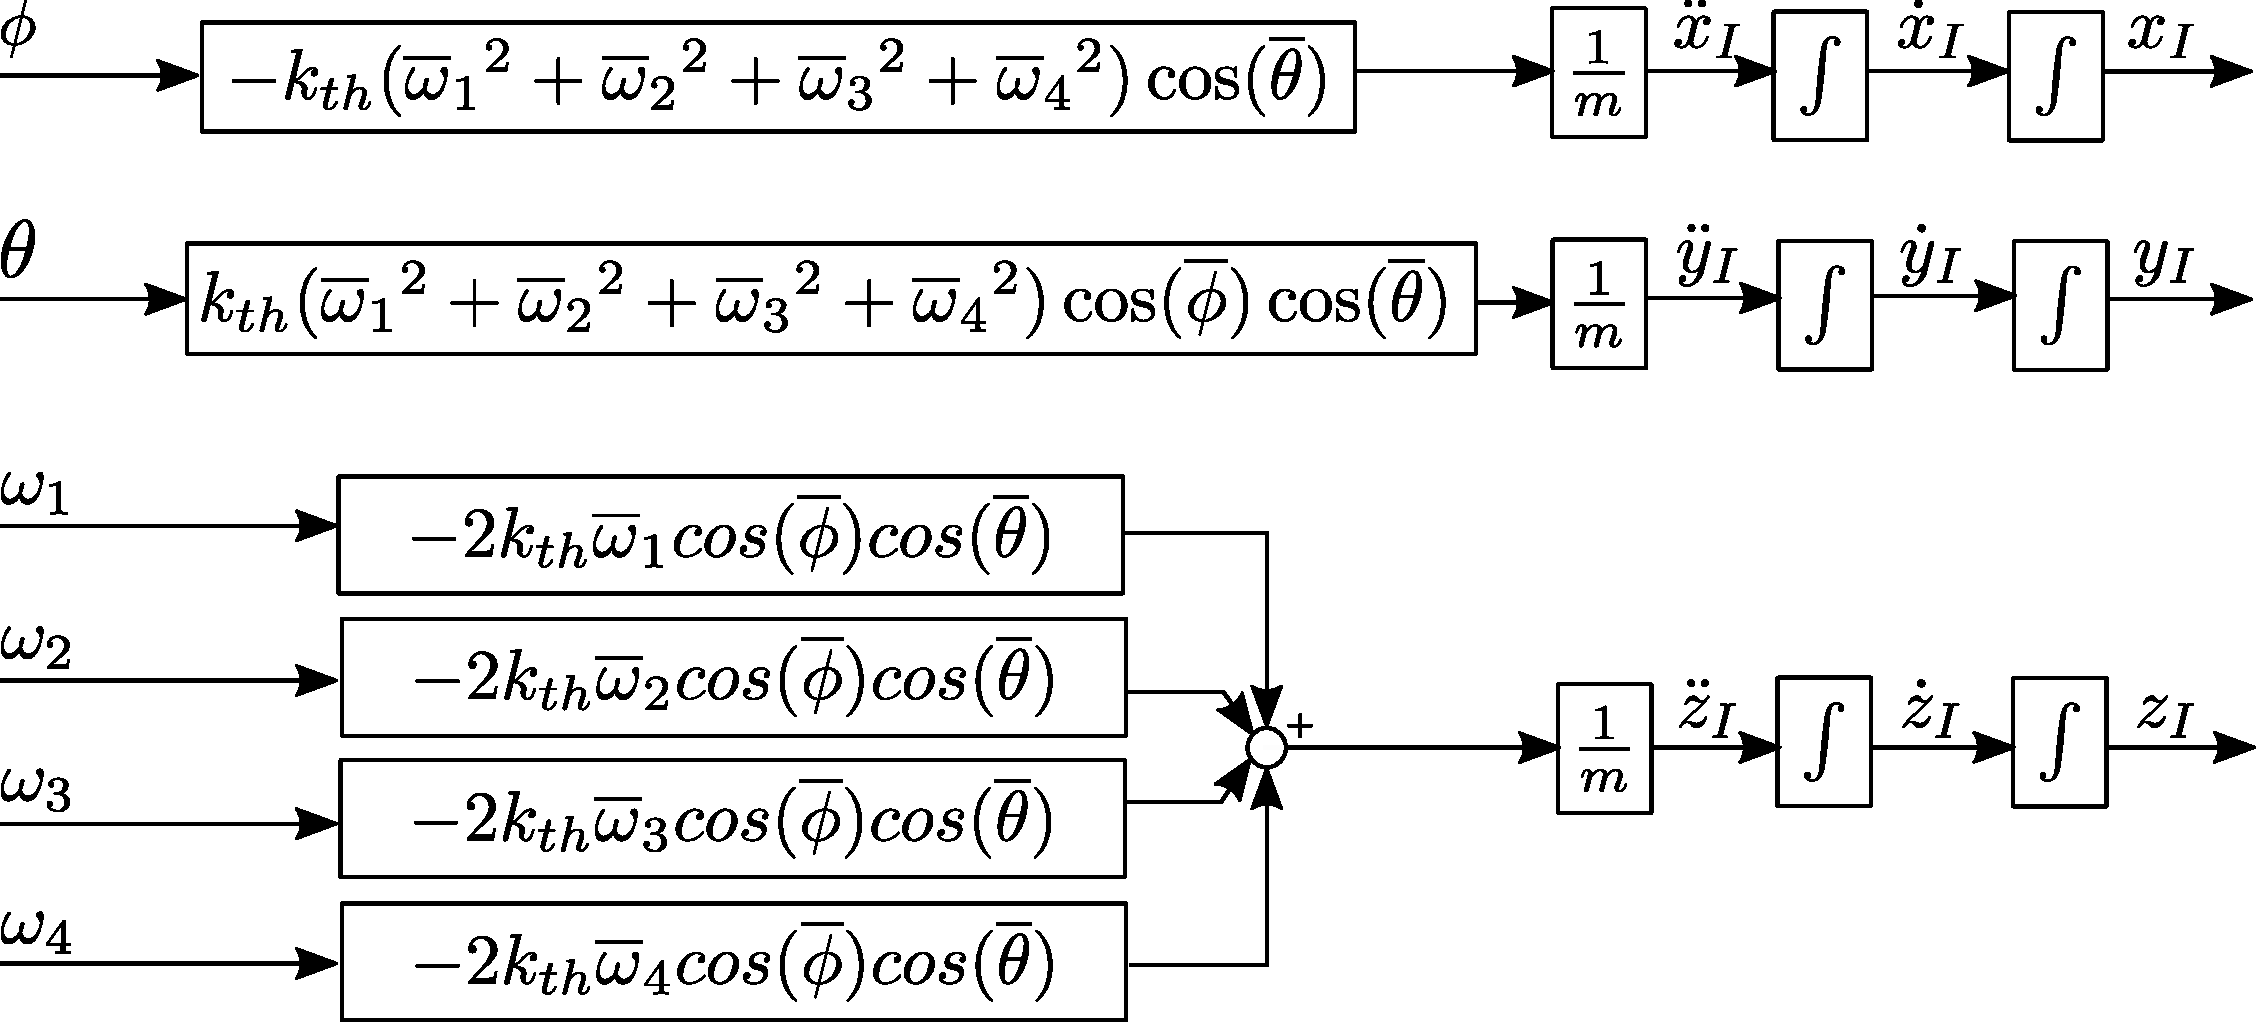
\includegraphics[scale=0.45]{figures/TranslationalLinearModelBlockDiagram.pdf}
	\caption{A block diagram of the translational model linear approximated equations. The input is the angular velocities of the four motors and the output is the three positions in x, y and z.}
	\label{fig:TranslationalLinearModelBlockDiagram}
\end{figure}

\subsection{Simulation}
The simulation of the model is done in Simulink. The parameters used for the simulations are shown in \autoref{ParametersQuadcopter}.
\begin{table}[H]
	\centering
	\begin{tabular}{|l|l|l|p{3cm}|}
		\hline %-----------------------------------------------------------------------------------
		\textbf{Parameter Name}&\textbf{Symbol} &\textbf{Value} &\textbf{Units}\\
		\hline %-----------------------------------------------------------------------------------
		Mass of the quadcopter  & $m$ & 0.996       &$kg$\\
		\hline
		%-----------------------------------------------------------------------------------
		Moment of inertia around x axis       & $J_x$  & 0.01073       & $kg \cdot m^2$\\
		\hline %-----------------------------------------------------------------------------------
		Moment of inertia around y axis       & $J_y$  & 0.01073       & $kg \cdot m^2$\\
		\hline %-----------------------------------------------------------------------------------
		Moment of inertia around z axis       & $J_z$  & 0.02135       & $kg \cdot m^2$\\
		\hline %-----------------------------------------------------------------------------------
		Length of quadcopter arm       & $L$  &   0.225       & $m$\\
		\hline %-----------------------------------------------------------------------------------
		Thrust force constant       & $k_{th}$  & -       & $N\cdot s^2 rad^{-2}$\\
		\hline %-----------------------------------------------------------------------------------\\
		Drag torque constant      & $k_{d}$  & -       & $Nm\cdot m^2 rad^{-2}$\\
		\hline %-----------------------------------------------------------------------------------\\
	\end{tabular}
	\caption{Parameters used in the simulation of the model.}
	\label{ParametersQuadcopter}
\end{table}\vspace{-18pt}

\subsubsection{Attitude Model Simulations}
In \autoref{fig:rollCompModel}, \ref{fig:pitchCompModel} and \ref{fig:yawCompModel}, the angular behavior of the model is analyzed. The input to the system are the four motor velocities. They are defined so the response of the model is predictable and the its performance can be evaluated.

The behavior around x axis is shown in \autoref{fig:rollCompModel}. Only the speeds of motors 2 and 4 are changed as they are supposed to be the ones that affect the roll angle. It can be seen that a positive difference in the rotation speed of these motors generates a positive acceleration in the roll direction, which is consistent with \autoref{eq:AngleEqVelocitiescombined1}.

It can also be observed that the linear approximation of the equations yields an accurate result as the two responses show no perceptible difference. 
%
\begin{figure}[H]
	\centering
	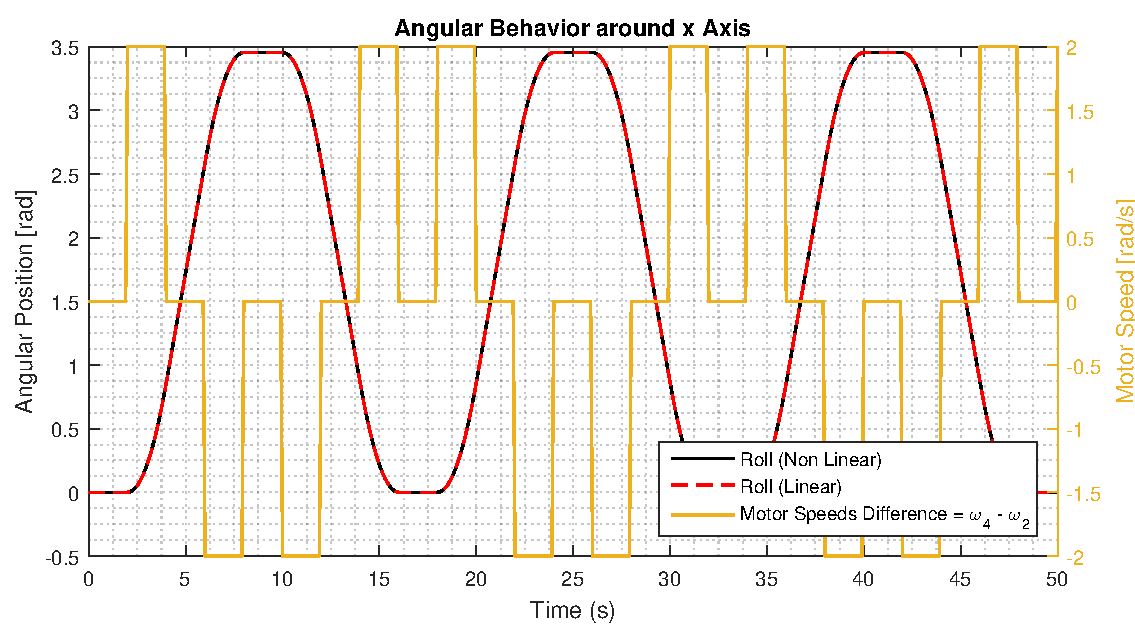
\includegraphics[scale=0.65]{figures/rollCompModel}
	\caption{Behavior of the non linear and linear models in roll angle.}
	\label{fig:rollCompModel}
\end{figure}
%
The behavior around the y axis is very similar to that of the roll angle. It is shown in \autoref{fig:pitchCompModel}. In this case, the motor velocities modified are those from motors 1 and 3. 
%
\autoref{eq:AngleEqVelocitiescombined2} states that a positive rotational speed difference creates a positive pitch acceleration. This is confirmed by the simulations in both models. Again, the linear approximation can be considered adequate.
\begin{figure}[H]
	\centering
	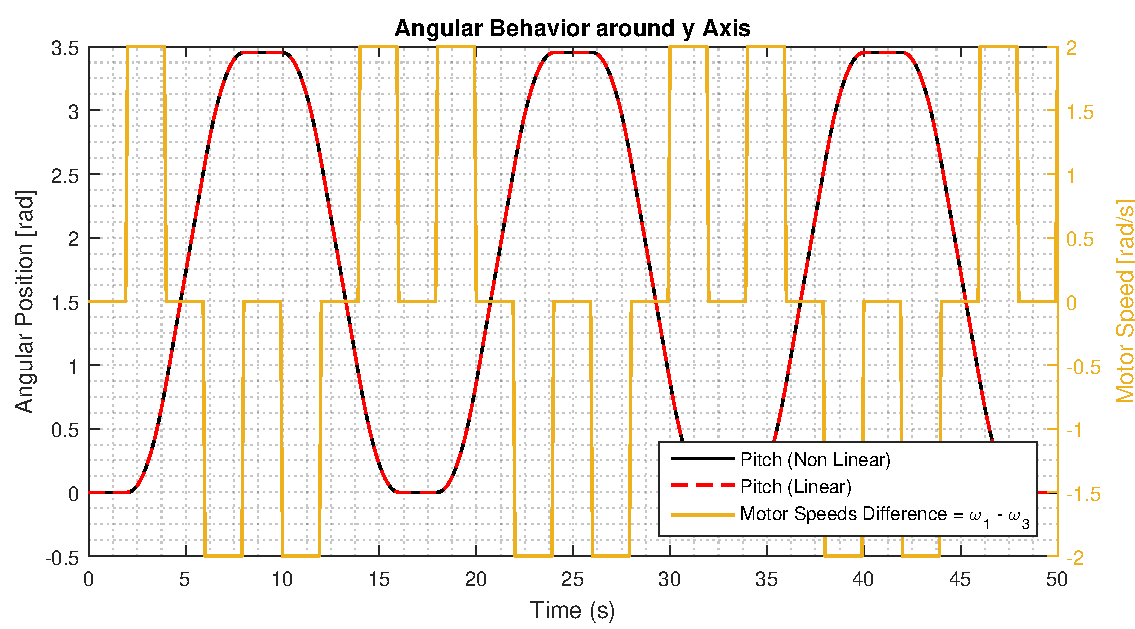
\includegraphics[scale=0.65]{figures/pitchCompModel}
	\caption{Behavior of the non linear and linear models in pitch angle.}
	\label{fig:pitchCompModel}
\end{figure}
%
The last attitude response simulated is around the z axis and is displayed in \autoref{fig:YawCompModel}. In this case all motor velocities affect the yaw angle. In the simulation, velocities of motors 1 and 3 are increased while those of motors 2 and 4 are decreased and vice versa. This creates yaw accelerations according to \autoref{eq:AngleEqVelocitiescombined3}. The response of the model is also correct and the linear approximation can be said to be accurate. 
%
\begin{figure}[H]
	\centering
	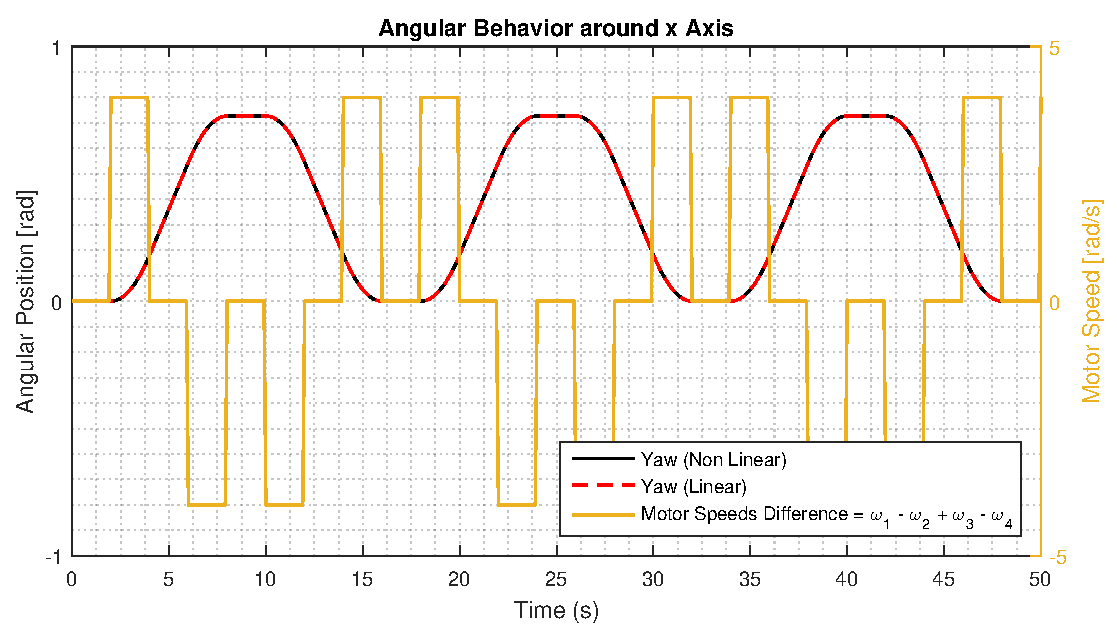
\includegraphics[scale=0.65]{figures/yawCompModel}
	\caption{Behavior of the non linear and linear models in yaw angle.}
	\label{fig:yawCompModel}
\end{figure}

\subsubsection{Translational Model Simulations}
The simulations carried out in the translational models are shown in  \autoref{fig:xCompModel}, \ref{fig:yCompModel} and \ref{fig:zCompModel}. The inputs for these model are roll and pitch angles and the addition of the four motor velocities. 

\autoref{fig:xCompModel} shows how the inertial position in the x axis evolves with constant velocities of the motors and a change in the pitch angle. As expected, a negative translational acceleration is generated for a positive angle change and that drives the position to negative values. This response follows \autoref{eq:AccelerationEqInertialVelocitiescombined1}. The linear approximation is considered suitable when looking at the linear model response.
\begin{figure}[H]
	\centering
	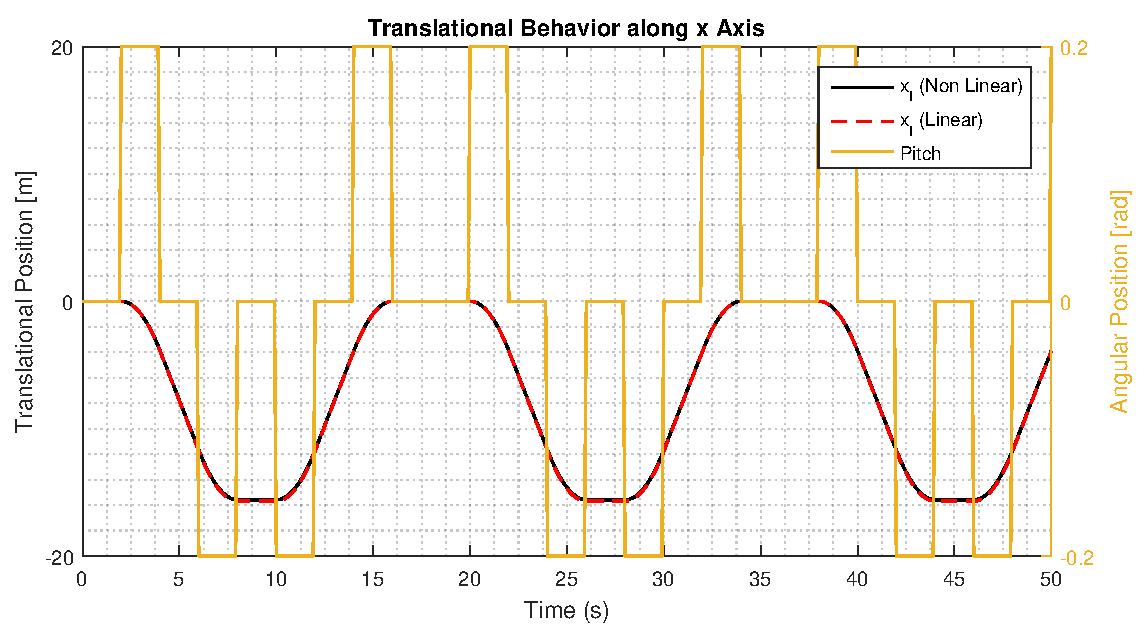
\includegraphics[scale=0.65]{figures/xCompModel}
	\caption{Behavior of the non linear and linear models along the x axis.}
	\label{fig:xCompModel}
\end{figure}
The response along the y inertial direction is depicted in \autoref{fig:yCompModel}. It is similar to that of the x direction but in this case a change in roll is needed to change the acceleration. Now, a positive roll angle generates a positive acceleration, as opposed to the x axis case. All goes in accordance with \autoref{eq:AccelerationEqInertialVelocitiescombined2}. As previously, the linear approximation performs well in the simulation.
\begin{figure}[H]
	\centering
	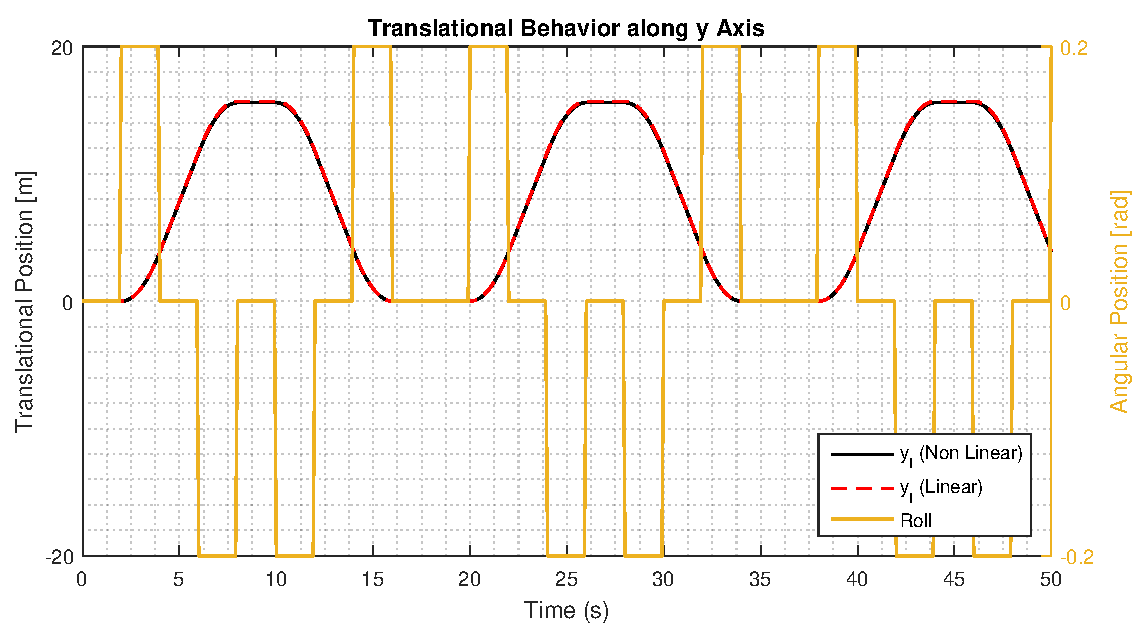
\includegraphics[scale=0.65]{figures/yCompModel}
	\caption{Behavior of the non linear and linear models along the y axis.}
	\label{fig:yCompModel}
\end{figure}
Finally, \autoref{fig:zCompModel} presents the behavior along the z axis. The pitch and roll angle are kept to zero and the summation of motor velocities are changed. For a higher sum, a more negative acceleration in the z axis is generated as it can be seen in \autoref{eq:AccelerationEqInertialVelocitiescombined3} and in the simulation through the z position. In this case, the linear approximation of the squared velocity term in the equations creates a difference in the output z position between the two models that is noticeable in the graph. This difference can be considered not to affect the system as the controller designed will handle it.  
\begin{figure}[H]
	\centering
	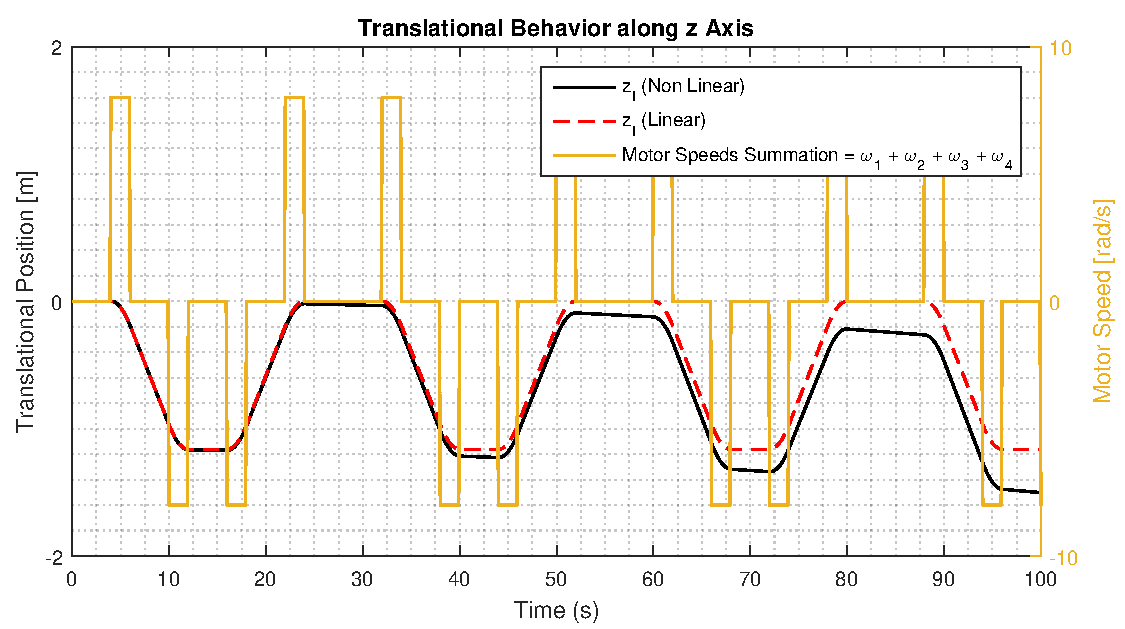
\includegraphics[scale=0.65]{figures/zCompModel}
	\caption{Behavior of the non linear and linear models along the z axis..}
	\label{fig:zCompModel}
\end{figure}

In this chapter, the attitude and translational models of the system have been derived. A linear approximation of the obtained equations will be used in the next chapter to design the necessary controllers to achieve the desired flight behavior for the quadcopter.





	
	%---------- Chapter 5 ----------------------------------------


	%%% Part 2 %%%
	\part{Design}	
		
	%---------- Chapter 6 ---------------------------------------- 	
	\chapter{Controller Design}\label{chap:Control}

Control Strategy (all the relations between controllers)\\
Flow of chapter\\	
	\section{Attitude Controller}
The angular response of the quadcopter constitutes a coupled behavior as the three Euler angles (\si{\phi}, \si{\theta} and  \si{\psi}) are affected by the four motor velocities. This makes it harder to utilize independent controllers for each angle. A state space approach is instead considered.   

In state space, the system behavior is represented by means of the linearized model equations. These show how the output and the states of the system evolve as a function of the current states values and the input applied to the system. \autoref{xDotDiffEq} and \autoref{yDiffEq} show the idea of state space representation.
%
\begin{flalign}
	\vec{\dot{x}}(t)&=f(\vec{x}(t),\vec{u}(t))
	\label{xDotDiffEq} 
\end{flalign}
\begin{flalign}
	\vec{y}(t)&=g(\vec{x}(t),\vec{u}(t)) 
	\label{yDiffEq} 
\end{flalign}
%
The description of the system can also be expressed in matrix form, giving \autoref{xDotLinear} and \autoref{yLinear}.
%
\begin{flalign}
	\vec{\dot{x}}(t)&=\vec{A} \  \vec{x}(t) + \vec{B} \  \vec{u}(t)
	\label{xDotLinear} 
\end{flalign}
\begin{flalign}
	\vec{y}(t)&=\vec{C} \  \vec{x}(t) + \vec{D} \  \vec{u}(t)
	\label{yLinear} 
\end{flalign}
%
\begin{where}
    \va{\vec{A}}{$=\frac{\partial}{\partial \vec{x} } \ f(\vec{x_o},\vec{u_o})$ \ \ is the $6 \times 6$ state feedback matrix}{}
    \va{\vec{B}}{$=\frac{\partial}{\partial \vec{u}} \ f(\vec{x_o},\vec{u_o})$ \ \ is the $6 \times 4$  input matrix}{}
    \va{\vec{C}}{$=\frac{\partial}{\partial \vec{x}} \ g(\vec{x_o},\vec{u_o})$ \ \ is the $3 \times 6$  output matrix}{}
    \va{\vec{D}}{$=\frac{\partial}{\partial \vec{u}} \ g(\vec{x_o},\vec{u_o})$ \ \ is the $3 \times 4$  feedforward matrix}{}
\end{where}

This state space description can be seen also in the form of a block diagram like the one shown in \autoref{SSBlocks}.
%
\begin{figure}[H]
	\begin{tikzpicture}[ auto,
                       thick,                         %<--setting line style
                       node distance=1.5cm,             %<--setting default node distance
                       scale=1,                     %<--|these two scale the whole thing
                       every node/.style={scale=1}, %<  |(always change both)
                       >=triangle 45 ]                %<--sets the arrowtype
    
    \draw%-----------------------------------------------------------------------------------------
    	%Drawing Input/Output:
    	node[shape=coordinate][](input1) at (0,0){}
    	node[shape=coordinate][](output1) at (9.5,0){}
     	%Drawing the Equation Blocks:   	
      	node(A) at (4.5,-1.5) [block] {A} 
     	node(B) at (1.5,0) [block] {B}
     	node(C) at (6.5,0) [block] {C}
      	node(D) at (4.5,1.5) [block] {D}  
	    node(int) at (4.5,0) [block] {\si{\int}}  
    	%Drawing the Sumation Blocks:	    	 	
    	node(sum1) [sum, right of = B] {\si{\sum}}
    	node(sum2) [sum, right of = C] {\si{\sum}}
    	%Drawing the Feedback/Feedforward Nodes:    	
    	node[shape=coordinate][](FeedforwardNode) at (0.75,0){}
    	node[shape=coordinate][](FeedbackNode) at (5.5,0){}  	
    	     
    ;%---------------------------------------------------------------------------------------------
   
    %Joining the Blocks
  	\draw[->](input1) -- node {u}(B);
  	\draw[->](B) -- node {}(sum1);
  	\draw[->](sum1) -- node {\si{\dot x}}(int);  	
  	\draw[->](int) -- node {x}(C);
  	\draw[->](C) -- node {}(sum2);  	
  	\draw[->](sum2) -- node {y}(output1);
  	
  	\draw[->](FeedforwardNode) |- node{} (D);
  	\draw[->](D) -| node{} (sum2);

  	\draw[-] (FeedbackNode) |- (A);
  	\draw[->] (A)   -| (sum1);

    %Drawing node(s) with \textbullet
    \draw%--------------------------------------------------------------
      node at (input1)  [shift={(-0.08, -0.02 )}] {\large \textbullet}
    	% node at (output1) [shift={( 0.008, -0.02 )}] {\textbullet}
    ;%------------------------------------------------------------------
  \end{tikzpicture}
	\centering
	\caption{Block diagram of the state space representation of the system.}
	\label{SSBlocks}
\end{figure}\vspace{-18pt}
%
As the orientation of the quadcopter is to be controlled and the differential equations that describe the behavior include the angular accelerations, the state vector is chosen to be formed by the angles and the angular velocities. The input vector contains the four motor velocities and the output is constructed by the angles \si{\phi}, \si{\theta}, \si{\psi}. These vectors can be seen in \autoref{uVector}.\\
\begin{minipage}{0.32\linewidth}
	\begin{flalign}
		\vec{x}(t) = 
		\begin{bmatrix}
			\phi \\
			\theta \\ 
			\psi \\
			\dot{\phi} \\
			\dot{\theta} \\
			\dot{\psi} \\
		\end{bmatrix}	\nonumber
		\label{xVector}
	\end{flalign}  
\end{minipage}\hfill
%\hspace{0.03\linewidth}
\begin{minipage}{0.32\linewidth}
	\begin{flalign}
		\vec{y}(t) = 
		\begin{bmatrix}
			\phi \\
			\theta \\ 
			\psi \\
		\end{bmatrix}	\nonumber
		\label{yVector}
	\end{flalign}
\end{minipage}\hfill
%\hspace{0.03\linewidth}
\begin{minipage}{0.32\linewidth}
	\begin{flalign}
		\vec{u}(t)= 
		\begin{bmatrix}
			\omega_1 \\
			\omega_2 \\
			\omega_3 \\
			\omega_4 \\
		\end{bmatrix}\textsl{}
		\label{uVector}
	\end{flalign}
\end{minipage}\hfill
\\
The specific matrices for the description of the angular behavior are obtained from the linearized equations of the system (\autoref{AngleLin1}, \ref{AngleLin2}) and they are showed embedded in the state space representation in \autoref{xDotSS} and \autoref{ySS}.

\begin{flalign}   \label{xDotSS}
	\vec{\dot{x}}(t) &=
	\begin{bmatrix}
		\ 0 & 0 & 0 & 1 & 0 & 0     \ \ \ \\ 
		\ 0 & 0 & 0 & 0 & 1 & 0     \ \ \ \\ 
		\ 0 & 0 & 0 & 0 & 0 & 1     \ \ \ \\
		\ 0 & 0 & 0 & 0 & 0 & 0     \ \ \ \\ 
		\ 0 & 0 & 0 & 0 & 0 & 0     \ \ \ \\ 
		\ 0 & 0 & 0 & 0 & 0 & 0     \ \ \ 		
	\end{bmatrix}
	\vec{x}(t) +
	\begin{bmatrix}
		\ 0 & 0 & 0 & 0      \ \ \ \\ 
		\ 0 & 0 & 0 & 0      \ \ \ \\ 
		\ 0 & 0 & 0 & 0      \ \ \ \\
		\ 0 & \si{-\frac{2 \  k_{th} \  L \  \overline{\omega}_2}{J_x}} & 0 & \si{\frac{2 \  k_{th} \  L \  \overline{\omega}_4}{J_x}}      \ \ \ \\ 
		\ \si{\frac{2 \  k_{th} \  L \  \overline{\omega}_1}{J_y}} & 0 & \si{-\frac{2 \  k_{th} \  L \  \overline{\omega}_3}{J_y}} & 0      \ \ \ \\ 
		\ \frac{2 \  k_d \  {\overline{\omega}_1}}{J_z} & - \frac{2 \  k_d \  {\overline{\omega}_2}}{J_z} & \frac{2 \  k_d \  {\overline{\omega}_3}}{J_z} & - \frac{2 \  k_d \  {\overline{\omega}_4}}{J_z}      \ \ \ 		
	\end{bmatrix}
	\vec{u}(t)
\end{flalign}
\begin{flalign} \label{ySS}
	\vec{y}(t) &=	 
	\begin{bmatrix}
		\ 1 & 0 & 0 & 0 & 0 & 0     \ \ \ \\ 
		\ 0 & 1 & 0 & 0 & 0 & 0     \ \ \ \\ 
		\ 0 & 0 & 1 & 0 & 0 & 0     \ \ \ 		
	\end{bmatrix}
	\vec{x}(t)
\end{flalign}


The dynamics of the system can be analyzed by looking at the system matrix A. The eigenvalues of this matrix represent the location of the open loop poles of the system. In this case, the system shows 6 poles located in zero, which means that the system is marginally stable. In order to place those poles at a better location state feedback is used together with an integral action to be able to set a desired reference for the angles that is different from zero. 

As the output is formed by the the three angles, these are the only measured states in the system. For doing the state feedback, the angular velocities are also needed. The way of obtaining it i chosen to be a reduce order observer even though when using the vicon system, the angular velocities could be estimated with a numerical differentiation procedure. The observer is more convenient in case of using on board sensors and by using it, that possibility is kept open.

This way of approaching the control of the system is simplified by the possibility of designing the state feedback and integral controller and the observer independently. This holds due to the separation principle \cite{ssReference}.

Before designing the controller and the observer, it is advisable to check the controllability and observability of the system. For doing so, the matrices shown in \autoref{controlabilityandobservability} are used.\\
\begin{minipage}{0.45\linewidth}
\begin{flalign}
\vec{{\mathcal C}} = 
\begin{bmatrix}
\vec{B}&\vec{A}\vec{B}&\vec{A^2}\vec{B}&\vec{A^3}\vec{B}&\vec{A^4}\vec{B}&\vec{A^5}\vec{B} \\	
\end{bmatrix}\nonumber 
\end{flalign}
\end{minipage}\hfill
%\hspace{0.03\linewidth}
\begin{minipage}{0.45\linewidth}
\begin{flalign}
\vec{{\mathcal O}} = 
\begin{bmatrix}
\vec{C} \\
\vec{C}\vec{A} \\
\vec{C}\vec{A}^2 \\
\vec{C}\vec{A}^3 \\
\vec{C}\vec{A}^4 \\
\vec{C}\vec{A}^5 \\		
\end{bmatrix}					\label{controlabilityandobservability} 									
\end{flalign}
\end{minipage}\hfill

The rank of these matrices is 6, that is, the number of states. This makes the system both controllable and observable. The precise value of the matrices can be seen in \autoref{app:matricesSS}.

The block diagram showing the system overview of the attitude controller is showed in \autoref{attitudecontrollerdiagram}, in which the state feedback, the integral control and the observer can be seen.
\begin{figure}[H]
	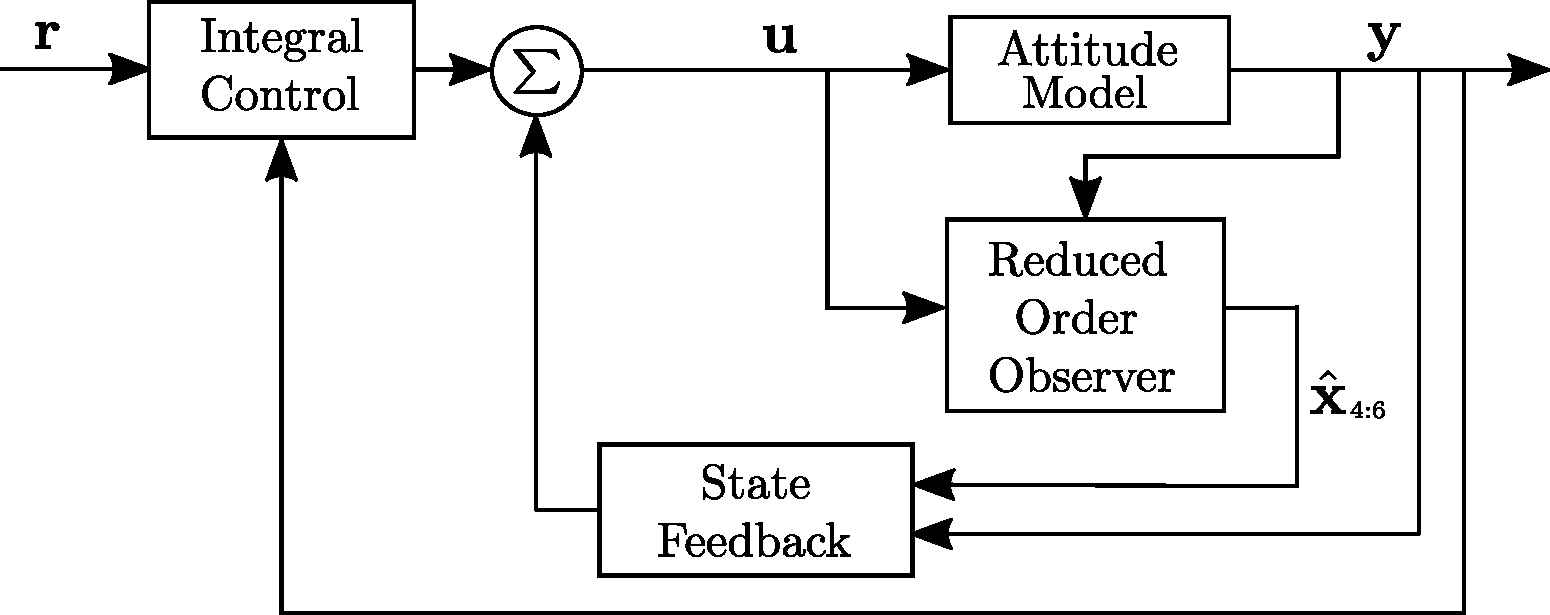
\includegraphics[scale=.5]{figures/AttitudeControlDiagram}
	\centering
	\caption{Control structure for the system, including the state feedback, the integral control and the reduced order observer.}
	\label{attitudecontrollerdiagram}
\end{figure}



	\subsection{State Feedback with Integral Control Design}
The aim of the controller is to be able to track a reference, within a reasonable range, in the three angles that define the attitude of the quadcopter.

Given a state space representation as the one in \autoref{xDotLinear} and \ref{yLinear}, it is possible to design a controller so that the final dynamics of the system can be chosen.

In this approach a state feedback is used to allow the system to return to equilibrium position while an integral controller makes it possible to include a reference and track it, adding both control actions to get the one finally applied to the motors. The diagram in \autoref{fig:DetailedControllerColorDiagram} shows how these controllers are related.
%
\begin{minipage}{\linewidth}
	\begin{minipage}{0.6\linewidth}
		\begin{figure}[H]
			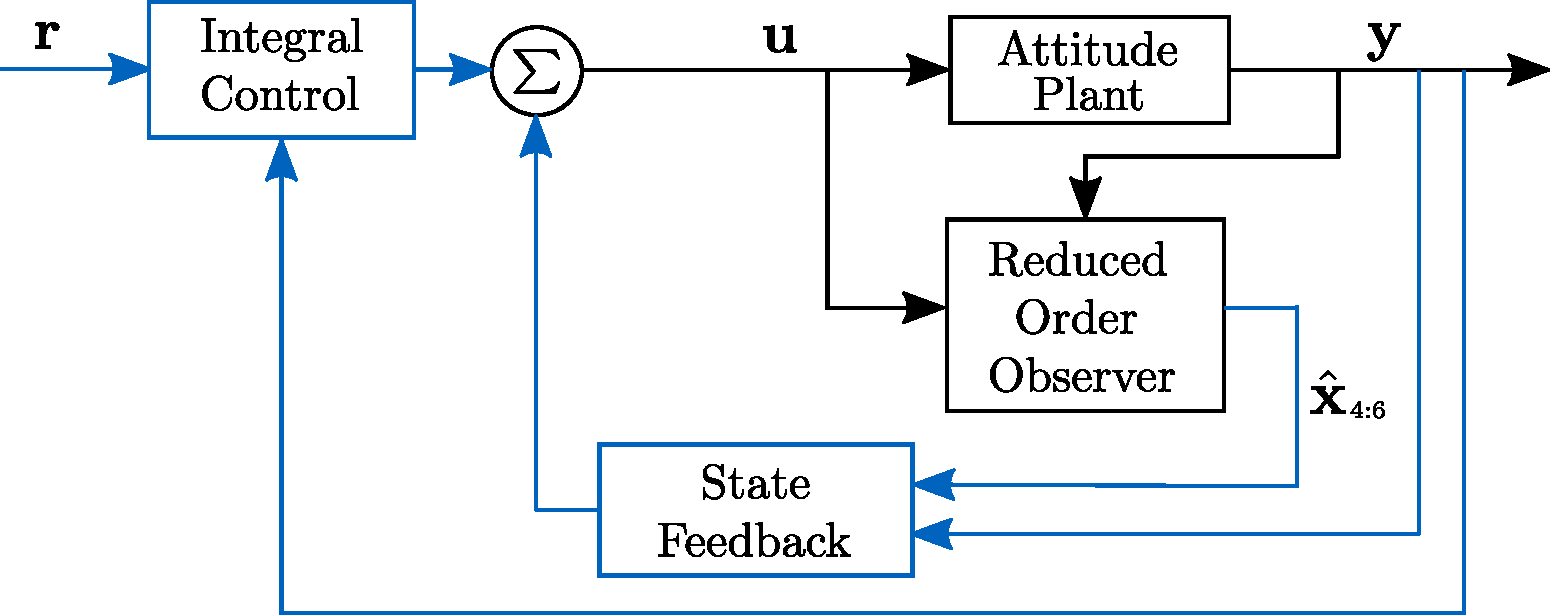
\includegraphics[scale=.35]{figures/ControllerColorDiagram}
			\centering			
			\captionof{figure}{Control structure with the state feedback and integral control parts highlighted.}
			\label{fig:ControllerColorDiagram}
		\end{figure}
	\end{minipage}
	\hspace{0.03\linewidth}
	\begin{minipage}{0.4\linewidth}
		\begin{figure}[H]\vspace{20mm}
			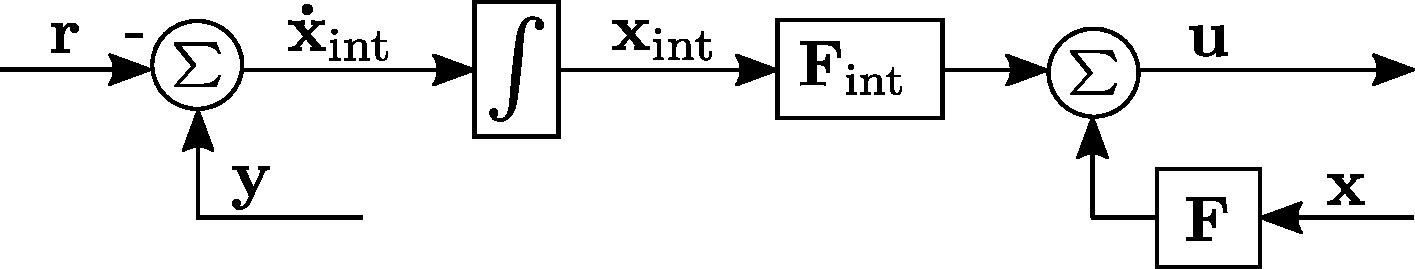
\includegraphics[scale=.35]{figures/DetailedControllerColorDiagram}
			\centering \vspace{7mm}
			\captionof{figure}{Detail of the left diagram, that includes all the variables used in the design of the controller.}
			\label{fig:DetailedControllerColorDiagram}
		\end{figure}
	\end{minipage}
\end{minipage}


From \autoref{fig:DetailedControllerColorDiagram}, the feedback law yields \autoref{eq:ssControllerAction}.
%
\begin{flalign} 
	\vec{u}(t) &=\vec{F} \  \vec{x}(t) + \ \vec{F}_{Int} \  \vec{x}_{Int}(t)
     \label{eq:ssControllerAction}
\end{flalign}
%
\begin{where}
	\va{\vec{F}}{is the 4x6 state feedback matrix}{}
	\va{\vec{F}_{Int}}{is the 3x6 integral feedback matrix }{}
\end{where}

In this equation, \si{\vec{x}_{Int}(t)} is given by \autoref{eq:ssControllerAction1}, that is equivalent to \autoref{eq:ssControllerAction2}, see \autoref{fig:DetailedControllerColorDiagram}.
\begin{flalign}
    \vec{x}_{Int}(t) &= \int_{0}^{t} \vec{y}(\tau)-\vec{r}(\tau) d\tau	\label{eq:ssControllerAction1}\\
    \vec{\dot{x}}_{Int}(t) &= \vec{y}(t)-\vec{r}(t) \label{eq:ssControllerAction2}
\end{flalign} 
%
This last equation can be introduced in the existing state space model, taking \si{\vec{x}_{Int}(t)} as new states, and giving the result shown in \autoref{xdotSSExtended} and \autoref{ySSExtended}.
%
\begin{flalign} 
    \dot{\vec{x}}_e(t) &= \vec{A}_e \  \vec{x}_e(t) + \vec{B}_e \  \vec{u}(t) + 
    \begin{bmatrix}
       \ \vec{0}     \ \ \ \\ 
       \ \vec{-I}     \ \ \  		
   \end{bmatrix}
   \vec{r}(t) 
   \label{xdotSSExtended}\\ 
    \vec{y}(t) &= \vec{C}_e \  \vec{x}_e 
       \label{ySSExtended}
\end{flalign} 
%
being\\
\begin{minipage}{0.24\linewidth}
	\begin{flalign}
		\dot{\vec{x}}_e(t)= 
		\begin{bmatrix}
			\ \dot{\vec{x}}(t)      \ \ \ \\ 
			\ \dot{\vec{x}}_{Int}(t)      \ \ \  		
		\end{bmatrix} \nonumber
	\end{flalign}
\end{minipage}\hfill
\begin{minipage}{0.24\linewidth}
	\begin{flalign}
	    \vec{A}_e=
	    \begin{bmatrix}
	        \ \vec{A}  & \vec{0}    \ \ \ \\ 
	        \ \vec{C}  & \vec{0}    \ \ \  		
	    \end{bmatrix} \nonumber
	\end{flalign}
\end{minipage}   \hfill 
\begin{minipage}{0.24\linewidth}
	\begin{flalign}
		\vec{B}_e=
		\begin{bmatrix}
			\ \vec{B}    \ \ \ \\ 
			\ \vec{0}     \ \ \  		
		\end{bmatrix} \nonumber
	\end{flalign}
\end{minipage}\hfill
\begin{minipage}{0.24\linewidth}
	\begin{flalign}
		\vec{C}_e=
		\begin{bmatrix}
			\ \vec{C}  & \vec{0}  \ \ \  		
		\end{bmatrix} \nonumber
	\end{flalign}
\end{minipage}

The resulting feedback law can be design as a conventional state feedback, where the goal is to choose an appropriate $F_e=[F \ F_{Int}]$ matrix such that the eigenvalues of $A_e+B_eF_e$ are the new poles that the system needs to have in order to achieve the desired dynamics.

Once $F_e$ is obtained, it can be splitted into $F$ and $F_{Int}$ by taking the first 6 columns for the state feedback and the last 3 for the integral control. In this way, the controller can be implemented as shown in \autoref{fig:DetailedControllerColorDiagram}.


 			  %----- Subsection
	\section{Reduced Order Observer Design}

\begin{flalign}  \label{observability}
	\vec{{\mathcal O}} = 
	\begin{bmatrix}
		\vec{C} \\
		\vec{C}\vec{A} \\
		\vec{C}\vec{A}^2 \\
		\vec{C}\vec{A}^3 \\
		\vec{C}\vec{A}^4 \\
		\vec{C}\vec{A}^5 \\		
	\end{bmatrix}
	\si{=}
	\begin{bmatrix}
		\ \ 1 & 0 & 0 & 0 & 0 & 0 \ \ \\
		\ \ 0 & 1 & 0 & 0 & 0 & 0 \ \ \\
		\ \ 0 & 0 & 1 & 0 & 0 & 0 \ \ \\
		\ \ 0 & 0 & 0 & 1 & 0 & 0 \ \ \\
		\ \ 0 & 0 & 0 & 0 & 1 & 0 \ \ \\
		\ \ 0 & 0 & 0 & 0 & 0 & 1 \ \ \\
		\ \ 0 & 0 & 0 & 0 & 0 & 0 \ \ \\
		\ \ 0 & 0 & 0 & 0 & 0 & 0 \ \ \\
		\ \ 0 & 0 & 0 & 0 & 0 & 0 \ \ \\
		\ \ 0 & 0 & 0 & 0 & 0 & 0 \ \ \\
		\ \ 0 & 0 & 0 & 0 & 0 & 0 \ \ \\
		\ \ 0 & 0 & 0 & 0 & 0 & 0 \ \ \\
		\ \ 0 & 0 & 0 & 0 & 0 & 0 \ \ \\
		\ \ 0 & 0 & 0 & 0 & 0 & 0 \ \ \\
		\ \ 0 & 0 & 0 & 0 & 0 & 0 \ \ \\
		\ \ 0 & 0 & 0 & 0 & 0 & 0 \ \ \\
		\ \ 0 & 0 & 0 & 0 & 0 & 0 \ \ \\
		\ \ 0 & 0 & 0 & 0 & 0 & 0 \ \ 														
	\end{bmatrix}
\end{flalign}

\begin{figure}[H]
	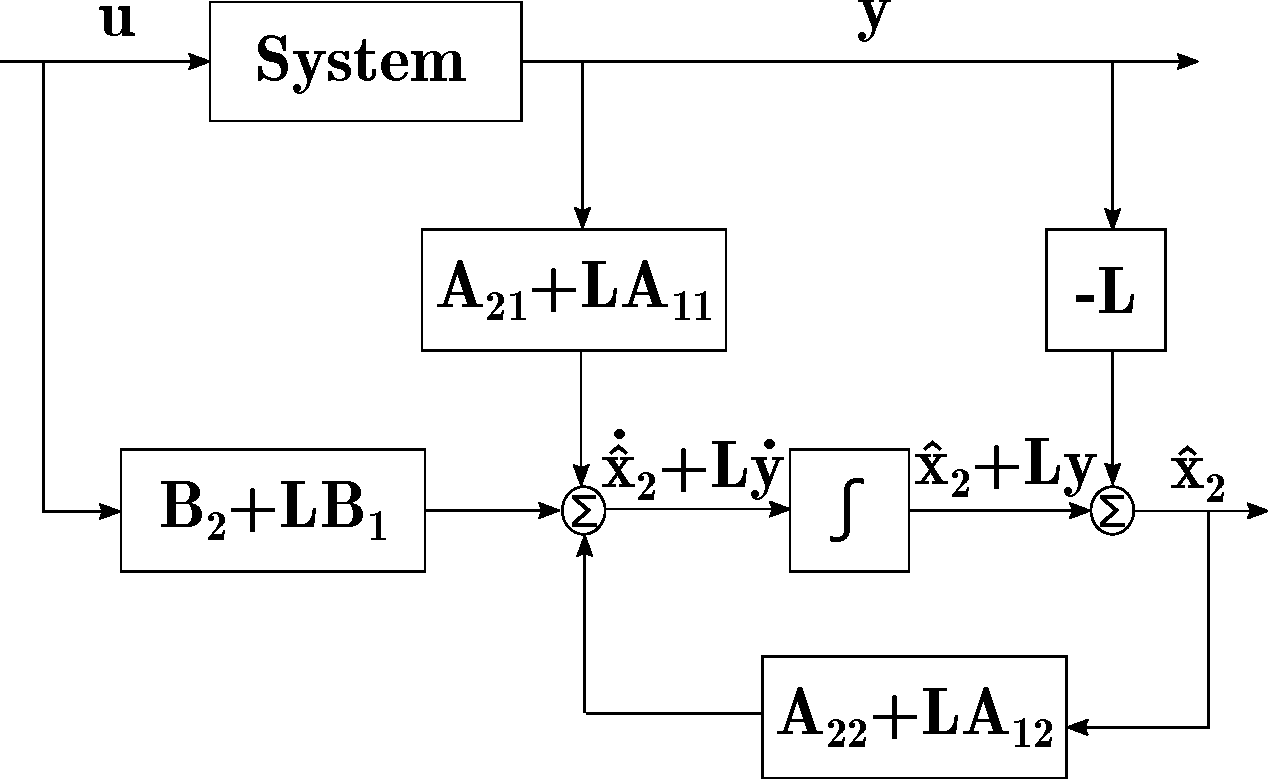
\includegraphics[scale=.35]{figures/observerDiagram}
	\centering
	\captionsetup{justification=centering}
	\captionof{figure}{Diagram . }
	\label{observerDiagram}
\end{figure}


\begin{minipage}{0.15\linewidth}
	\begin{flalign}
	A_{11} = 
	\begin{bmatrix}
		\ 0 & 0 & 0 \ \ \\ 
		\ 0 & 0 & 0 \ \ \\ 
		\ 0 & 0 & 0 \ \ \\
	\end{bmatrix}	\nonumber
	\label{A11}
	\end{flalign}  
\end{minipage}\hfill
\begin{minipage}{0.15\linewidth}
	\begin{flalign}
	A_{12} = 
	\begin{bmatrix}
		\ 1 & 0 & 0 \ \ \\ 
		\ 0 & 1 & 0 \ \ \\ 
		\ 0 & 0 & 1 \ \ \\
	\end{bmatrix}	\nonumber
	\label{A12}
	\end{flalign}
\end{minipage}\hfill
\begin{minipage}{0.15\linewidth}
	\begin{flalign}
	A_{21} = 
	\begin{bmatrix}
		\ 0 & 0 & 0 \ \ \\ 
		\ 0 & 0 & 0 \ \ \\ 
		\ 0 & 0 & 0 \ \ \\
	\end{bmatrix}	\nonumber
	\label{A21}
	\end{flalign}
\end{minipage}\hfill
\begin{minipage}{0.15\linewidth}
	\begin{flalign}
	A_{22} = 
	\begin{bmatrix}
		\ 0 & 0 & 0 & 0 \ \ \\ 
		\ 0 & 0 & 0 & 0 \ \ \\ 
		\ 0 & 0 & 0 & 0 \ \ \\
	\end{bmatrix} 
	\label{A22}
	\end{flalign}
\end{minipage}\hfill


\begin{minipage}{0.5\linewidth}
	\begin{flalign}
	B_1 = 
	\begin{bmatrix}
		\ 0 & 0 & 0 & 0 \ \ \\ 
		\ 0 & 0 & 0 & 0 \ \ \\ 
		\ 0 & 0 & 0 & 0 \ \ \\
	\end{bmatrix}	\nonumber
	\label{B1}
	\end{flalign}
\end{minipage}\hfill
\begin{minipage}{0.5\linewidth}
	\begin{flalign}
	B_2 = 
	\begin{bmatrix}
		0 & \si{-\frac{2 \cdot k_{th} \cdot L \cdot \overline{\omega}_2}{J_x}} & 0 & \si{\frac{2 \cdot k_{th} \cdot L \cdot \overline{\omega}_4}{J_x}} \ \ \ \\ 
		\ \si{\frac{2 \cdot k_{th} \cdot L \cdot \overline{\omega}_1}{J_y}} & 0 & \si{-\frac{2 \cdot k_{th} \cdot L \cdot \overline{\omega}_3}{J_y}} & 0 \ \ \ \\ 
		\frac{2 \cdot k_d \cdot {\overline{\omega}_1}}{J_z} & - \frac{2 \cdot k_d \cdot {\overline{\omega}_2}}{J_z} & \frac{2 \cdot k_d \cdot {\overline{\omega}_3}}{J_z} & - \frac{2 \cdot k_d \cdot {\overline{\omega}_4}}{J_z} \ \ \
	\end{bmatrix}
	\label{B2}
	\end{flalign}
\end{minipage}\hfill


\begin{flalign}
	L = 
	\begin{bmatrix}
	\ -50 & 0 & 0  \ \ \ \\ 
	\ 0 & -60 & 0  \ \ \ \\ 
	\ 0 & 0 & -70  \ \ \  
	\end{bmatrix}
	\label{Lobs}
\end{flalign}


 				  %----- Subsection
	%\subsection{Reduced Order Observer Design with Reference Signals}
Explain what is it\\
Diagram with colors + Block diagram\\
Equations\\
Simulation??\\

\begin{flalign}
	\eq{\vec{\vec{\dot{x}}(t)}}{\vec{A} \cdot \vec{x(t)} + \vec{B_1} (\vec{F}\vec{\hat{x}} + \vec{N}\vec{r})}
	%\label{xDotLinear} 
\end{flalign}


\begin{flalign}
	\eq{\vec{\dot{x}_1}(t)}{\vec{A_11} \cdot \vec{x_1}(t) + \vec{A_{12}} \cdot \vec{x_2}(t) + \vec{B_1}(F_1x_1 + F_2\hat{x}_2 + Nr)}
	%\label{xDotLinear} 
\end{flalign}

\begin{flalign}
	\eq{\vec{\dot{x}_2}(t)}{\vec{A_{21}} \cdot \vec{x_1}(t) + \vec{A_{22}} \cdot \vec{x_2}(t) + \vec{B_1}(F_1x_1 + F_2\hat{x}_2 + Nr)}
	%\label{xDotLinear} 
\end{flalign}

	\begin{flalign}
		\vec{y(t)} = \big(I \quad 0 \quad 0\big)
		\begin{pmatrix}
			\phi \\
			\theta \\ 
		\end{pmatrix}	\nonumber
		\label{yVector}
	\end{flalign}

\begin{flalign}
	\eq{\vec{\hat{\dot{x}}_2}(t)}{\vec{A_{21}} \cdot \vec{x_1}(t) + \vec{A_{22}} \cdot \vec{x_2}(t) + \vec{B_1}(F_1x_1 + F_2\hat{x_2} + Nr)}
	%\label{xDotLinear} 
\end{flalign}

						  %----- Subsection
	
	
%	
	%%% Part 3 %%%
	\part{Test \& Conclusion}
	
	%%% Setup for Appendix and Bibliography %%%

	
	\bookmarksetup{startatroot}
	\addtocontents{toc}{\bigskip}
	\newpage
	\fancyhead[RO]{\color{aaublue}\small Appendix \nouppercase\rightmark} %even page - chapter title
	\fancyhead[LE]{\color{aaublue}\small Appendix \nouppercase\rightmark} %uneven page - section title
	\fancyhead[RE,LO]{}
	\titleformat{\section}[hang]{\Large\bfseries}{\thesection\hsp\textcolor{aaublue}{|}\hsp}{0pt}{\Large\bfseries}

	%%% Appendix %%%
		%\renewcommand{\thechapter}{\Alph{chapter}}
		%	\addcontentsline{toc}{chapter}{Appendix}
		%	\setcounter{chapter}{0}
		%	\setcounter{section}{0}
		%	\setcounter{table}{0}
		%	\setcounter{equation}{0}
		%	\setcounter{figure}{0}


	\appendix
	\part*{Appendix} \addcontentsline{toc}{chapter}{Appendix}
	\cleardoublepage\makeatletter\@openrightfalse\makeatother
	
	
	%---------- Appendix A ----------------------------------------
	\chapter{Thrust Force Constant}\label{app:ThrustTest} 
\textbf{Name: Group 733}\\
\textbf{Date: 30/09 - 2016}

\subsubsection{Purpose}
Finding the relation between the speed of the motor and the thrust force generated by the propeller.

\subsubsection{Setup}
\begin{figure}[H]
	\centering
	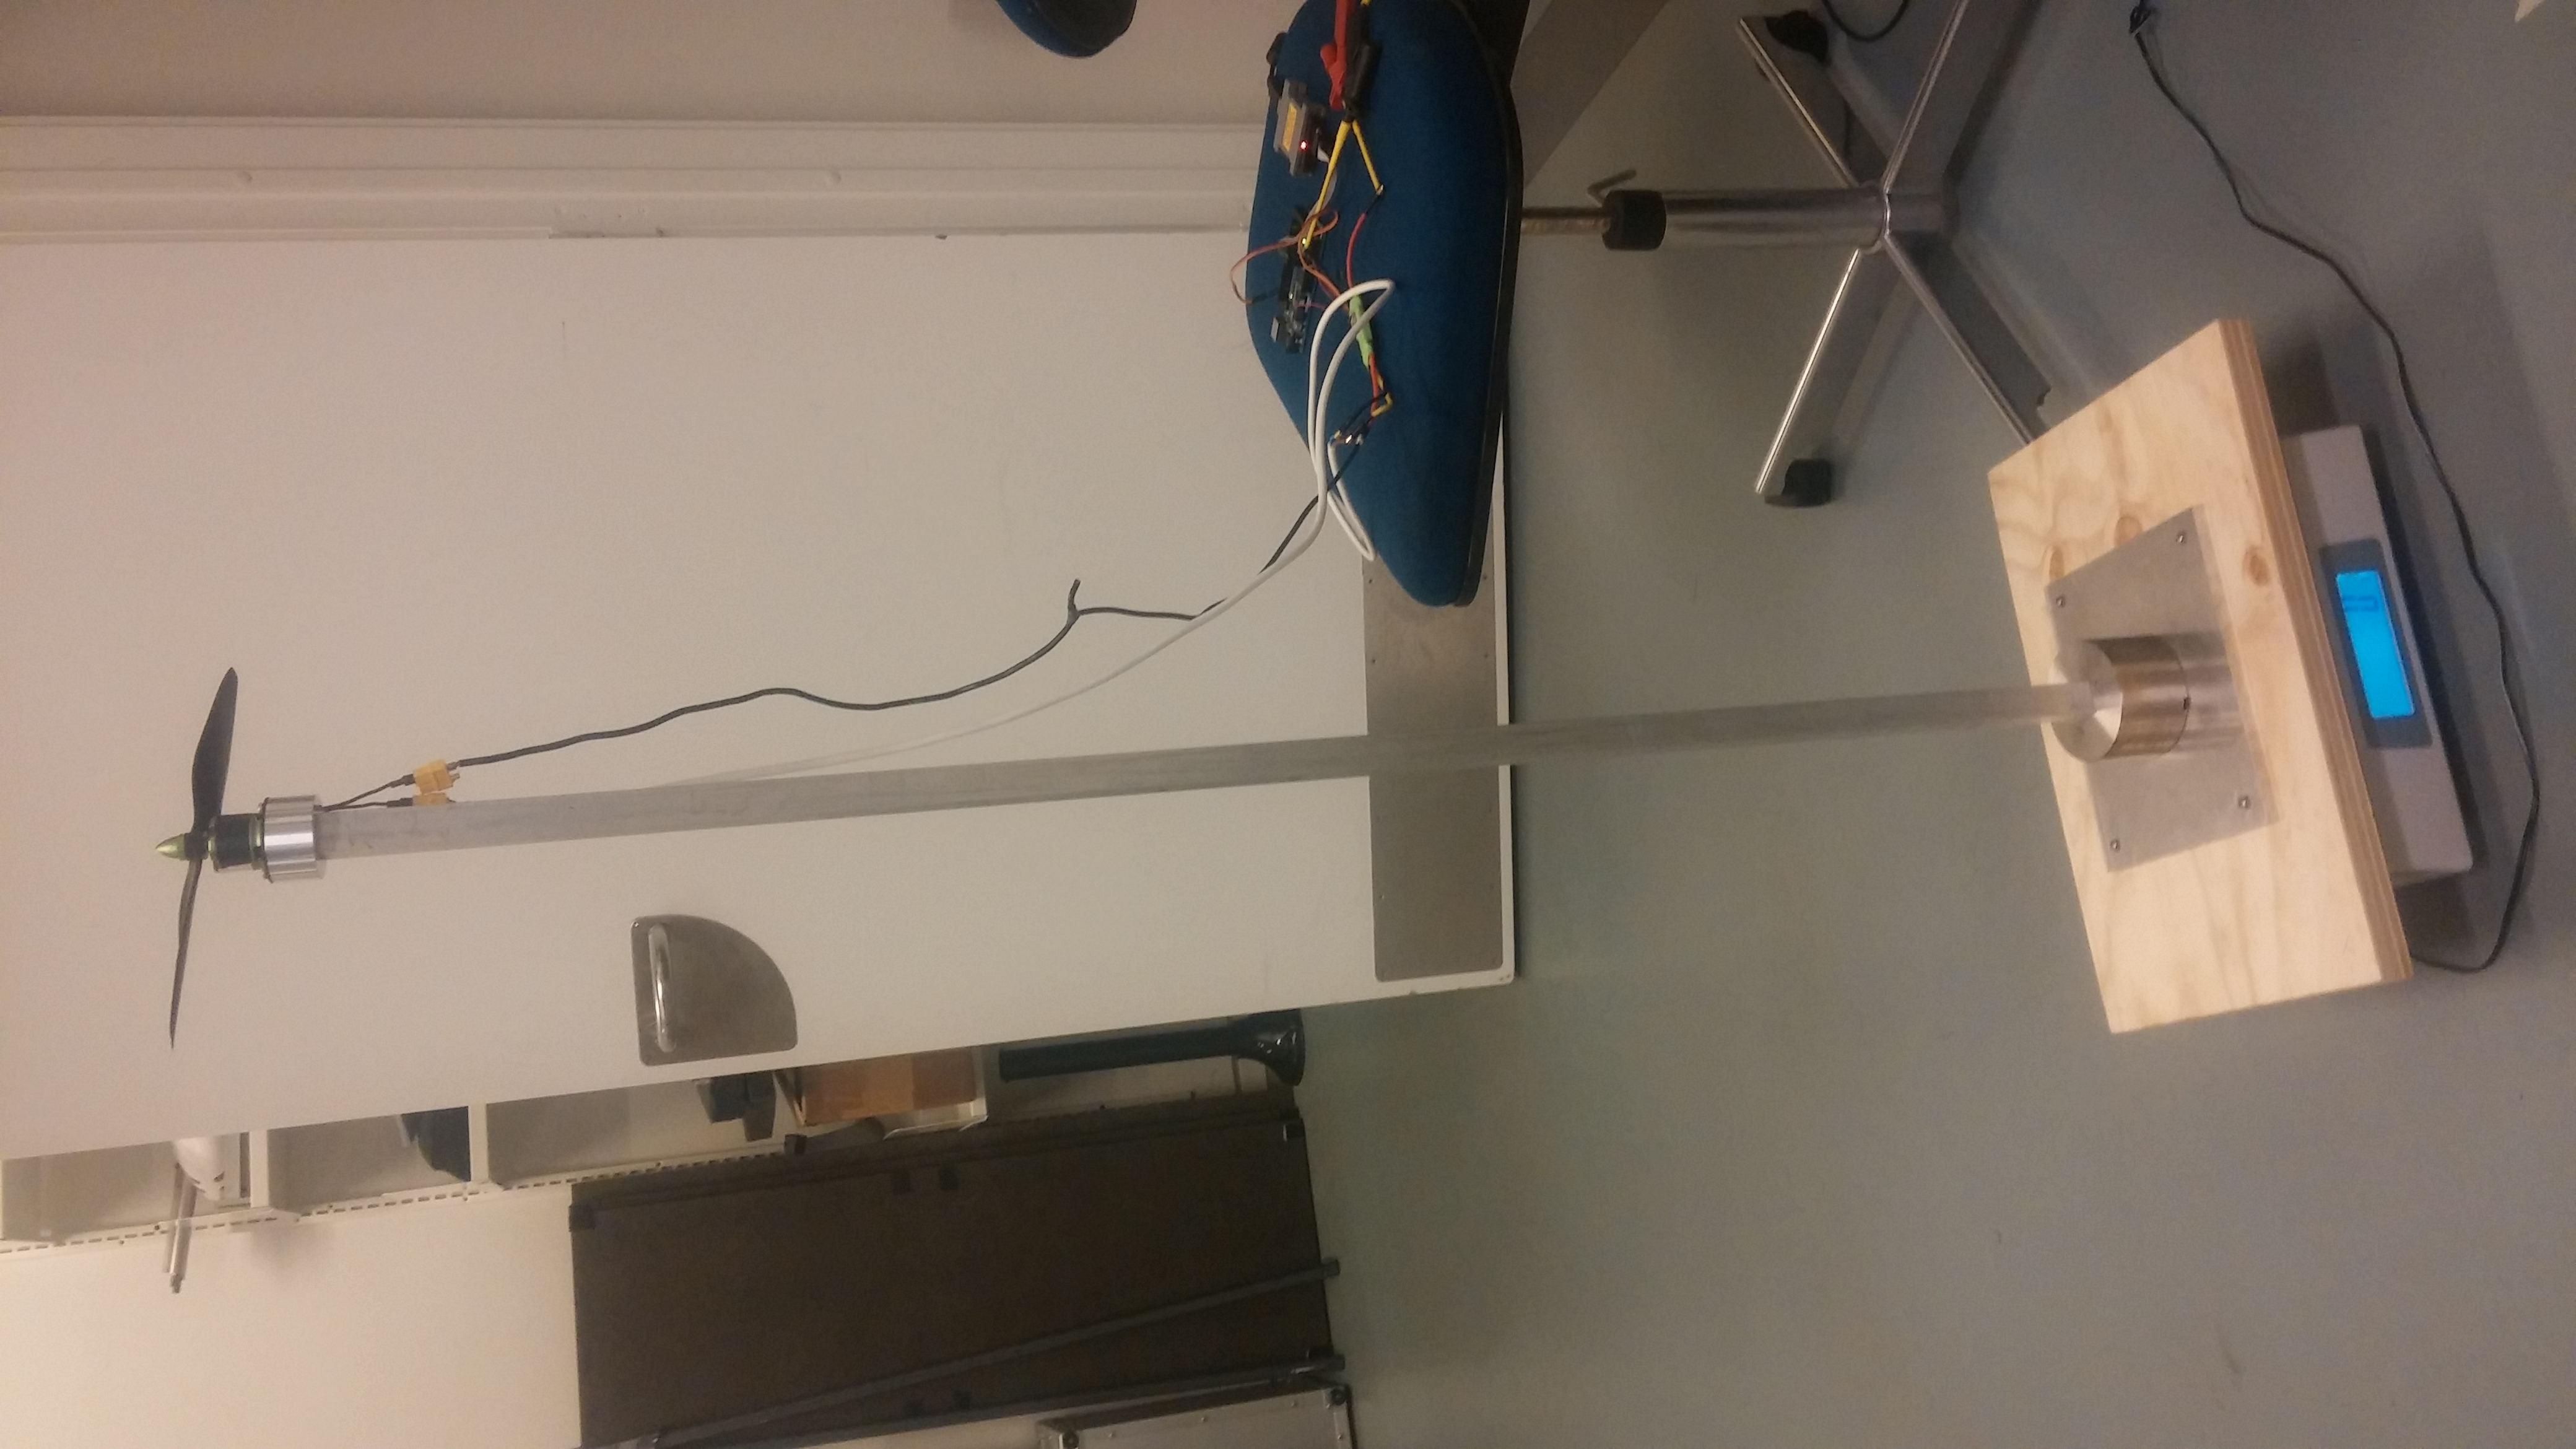
\includegraphics[scale=0.05,angle =-90]{figures/ThrustTestSetup}
	\caption{The setup for the thrust test.}
	\label{ThrustTest}
\end{figure}

\subsubsection{List of Equipment}
\begin{table}[H]
	\begin{tabular}{|l|l|p{4.3cm}|}
		\hline%------------------------------------------------------------------------------------------------------------
		\textbf{Instrument}                                  &  \textbf{AAU-no.}  &  \textbf{Type}                       \\
		\hline%------------------------------------------------------------------------------------------------------------
		Tachometer                                           &  08246           &  Shimpo DT-205		                   \\
		\hline%------------------------------------------------------------------------------------------------------------
	    Power Supply (11.1 V) &  64565                   &  ES 030-5                 \\
		\hline%------------------------------------------------------------------------------------------------------------
		Processing Unit                                   &  N/A               & Arduino Mega     \\
		\hline%------------------------------------------------------------------------------------------------------------
		Motor                                   &  N/A               & Multistar 2213-935     \\
		\hline%------------------------------------------------------------------------------------------------------------
		Motor Speed Controller                                   &  N/A               &  -      \\
		\hline%------------------------------------------------------------------------------------------------------------
		Propeller                                   &  N/A               & Turnigy 1045R     \\
		\hline%------------------------------------------------------------------------------------------------------------
		Scale                                  &  86759              & KERN FCB 12K1     \\
		\hline%------------------------------------------------------------------------------------------------------------
		
	\end{tabular}
\end{table}

\subsubsection{Procedure}
\begin{enumerate}
	\item Construct the setup as seen in \figref{ThrustTest}, the power supply is connected to the motor driver and the Arduino Mega is powered from the computer. One PWM pin and GND pin from the board must be connected to the driver signal cables yellow and brown respectively. 
	\item Run the program. It should generate a fixed duty PWM signal in the PWM pin.
	\item Wait for the speed to stabilize and read the scale value. The thrust force is calculated by multiplying the added mass in kilograms with the gravitational acceleration (\si{9,81\textbf{ }m/s^2})
	\item Measure the rotational speed with the tachometer.
\end{enumerate}


\subsubsection{Results}
\begin{table}[H]
	\centering
	\begin{tabular}{|l|l|l|l|p{4.3cm}|}
		\hline%------------------------------------------------------------------------------------------------------------
		\textbf{Motor Speed [rpm]}    & \textbf{Motor Speed [rad/s]} & \textbf{Added Mass [g]}  & \textbf{Thrust Force [N]} \\ 
		\hline%------------------------------------------------------------------------------------------------------------
		2240                        	   &  117,29                           & 69                       & 0,68         \\
		\hline%------------------------------------------------------------------------------------------------------------
		2305 						       &  120,69				           & 74                       & 0,73         \\
		\hline%------------------------------------------------------------------------------------------------------------
		2445                               &  128,02   			               & 85                       & 0,83         \\
		\hline%------------------------------------------------------------------------------------------------------------
		2495                               &  130,63  			               & 89                       & 0,87         \\
		\hline%------------------------------------------------------------------------------------------------------------
		2585                               &  135,35                           & 97                       & 0,95         \\
		\hline%------------------------------------------------------------------------------------------------------------
		2665 						       &  139,54				           & 99                       & 0,97         \\
		\hline%------------------------------------------------------------------------------------------------------------
		2811                               &  147,18    			           & 114                      & 1,12         \\
		\hline%------------------------------------------------------------------------------------------------------------
		2995                               &  156,82                           & 129                      & 1,27         \\
		\hline%------------------------------------------------------------------------------------------------------------
		3195 						       &  167,29				           & 150                      & 1,47         \\
		\hline%------------------------------------------------------------------------------------------------------------
		3287                               &  172,11   			               & 160                      & 1,57         \\
		\hline%------------------------------------------------------------------------------------------------------------
		3493                               &  182,89                           & 182                      & 1,79         \\
		\hline%------------------------------------------------------------------------------------------------------------
		3609 					           &  188,97	                       & 195                      & 1,91         \\
		\hline%------------------------------------------------------------------------------------------------------------
		3765 						       &  197,13		                   & 215                      & 2,11         \\
		\hline%------------------------------------------------------------------------------------------------------------
		3888 						       &  203,57		                   & 228                      & 2,23         \\
		\hline%------------------------------------------------------------------------------------------------------------
		4060 						       &  212,58		                   & 250                      & 2,46         \\
		\hline%------------------------------------------------------------------------------------------------------------
				
	\end{tabular}
\end{table}
\subsubsection{Results}
The obtained results are shown in \figref{ThrustGraph}. They have been approximated by a parabolic curve by finding a linear relation between the velocity squared and the thrust force.

\begin{figure}[H]
	\centering
	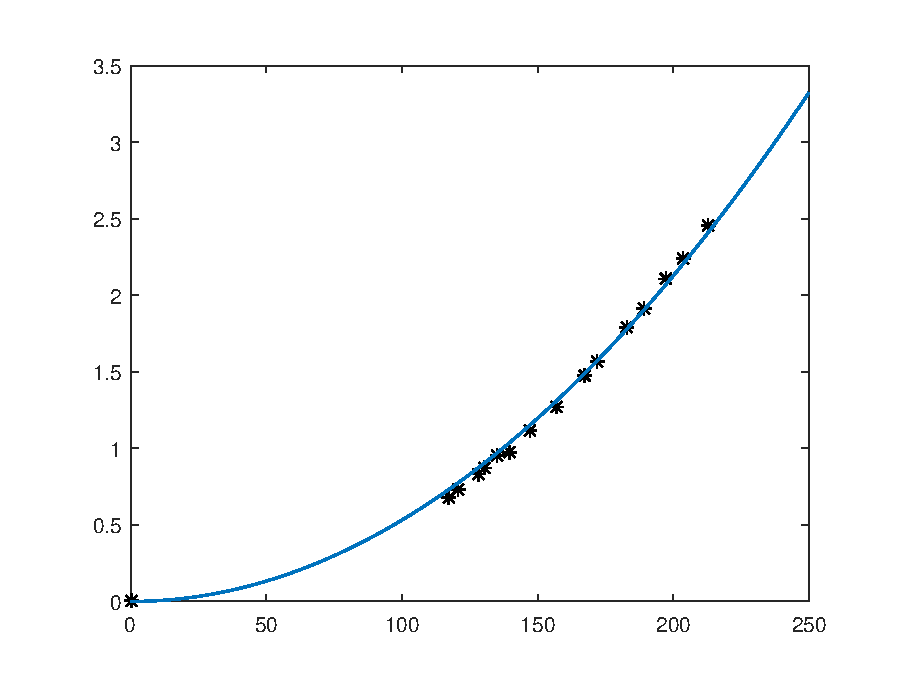
\includegraphics[scale=0.8]{figures/ThrustGraph.eps}
	\caption{Data from the thrust test approximated by a parabolic curve.}
	\label{ThrustGraph}
\end{figure}

The resulting constant that provides the relation between the thrust force in the propeller and the velocity squared is \si{5,316868\cdot10^{-5} N\cdot s^2/rad^2}.

	\chapter{Drag Torque Constant}\label{app:TorqueTest} 
\textbf{Name: Group 733}\\
\textbf{Date: 04/10 - 2016}

\subsubsection{Purpose}
Finding the relation between the speed of the motor and the drag torque generated by the propeller.

\subsubsection{Setup}
\begin{figure}[H]
	\centering
	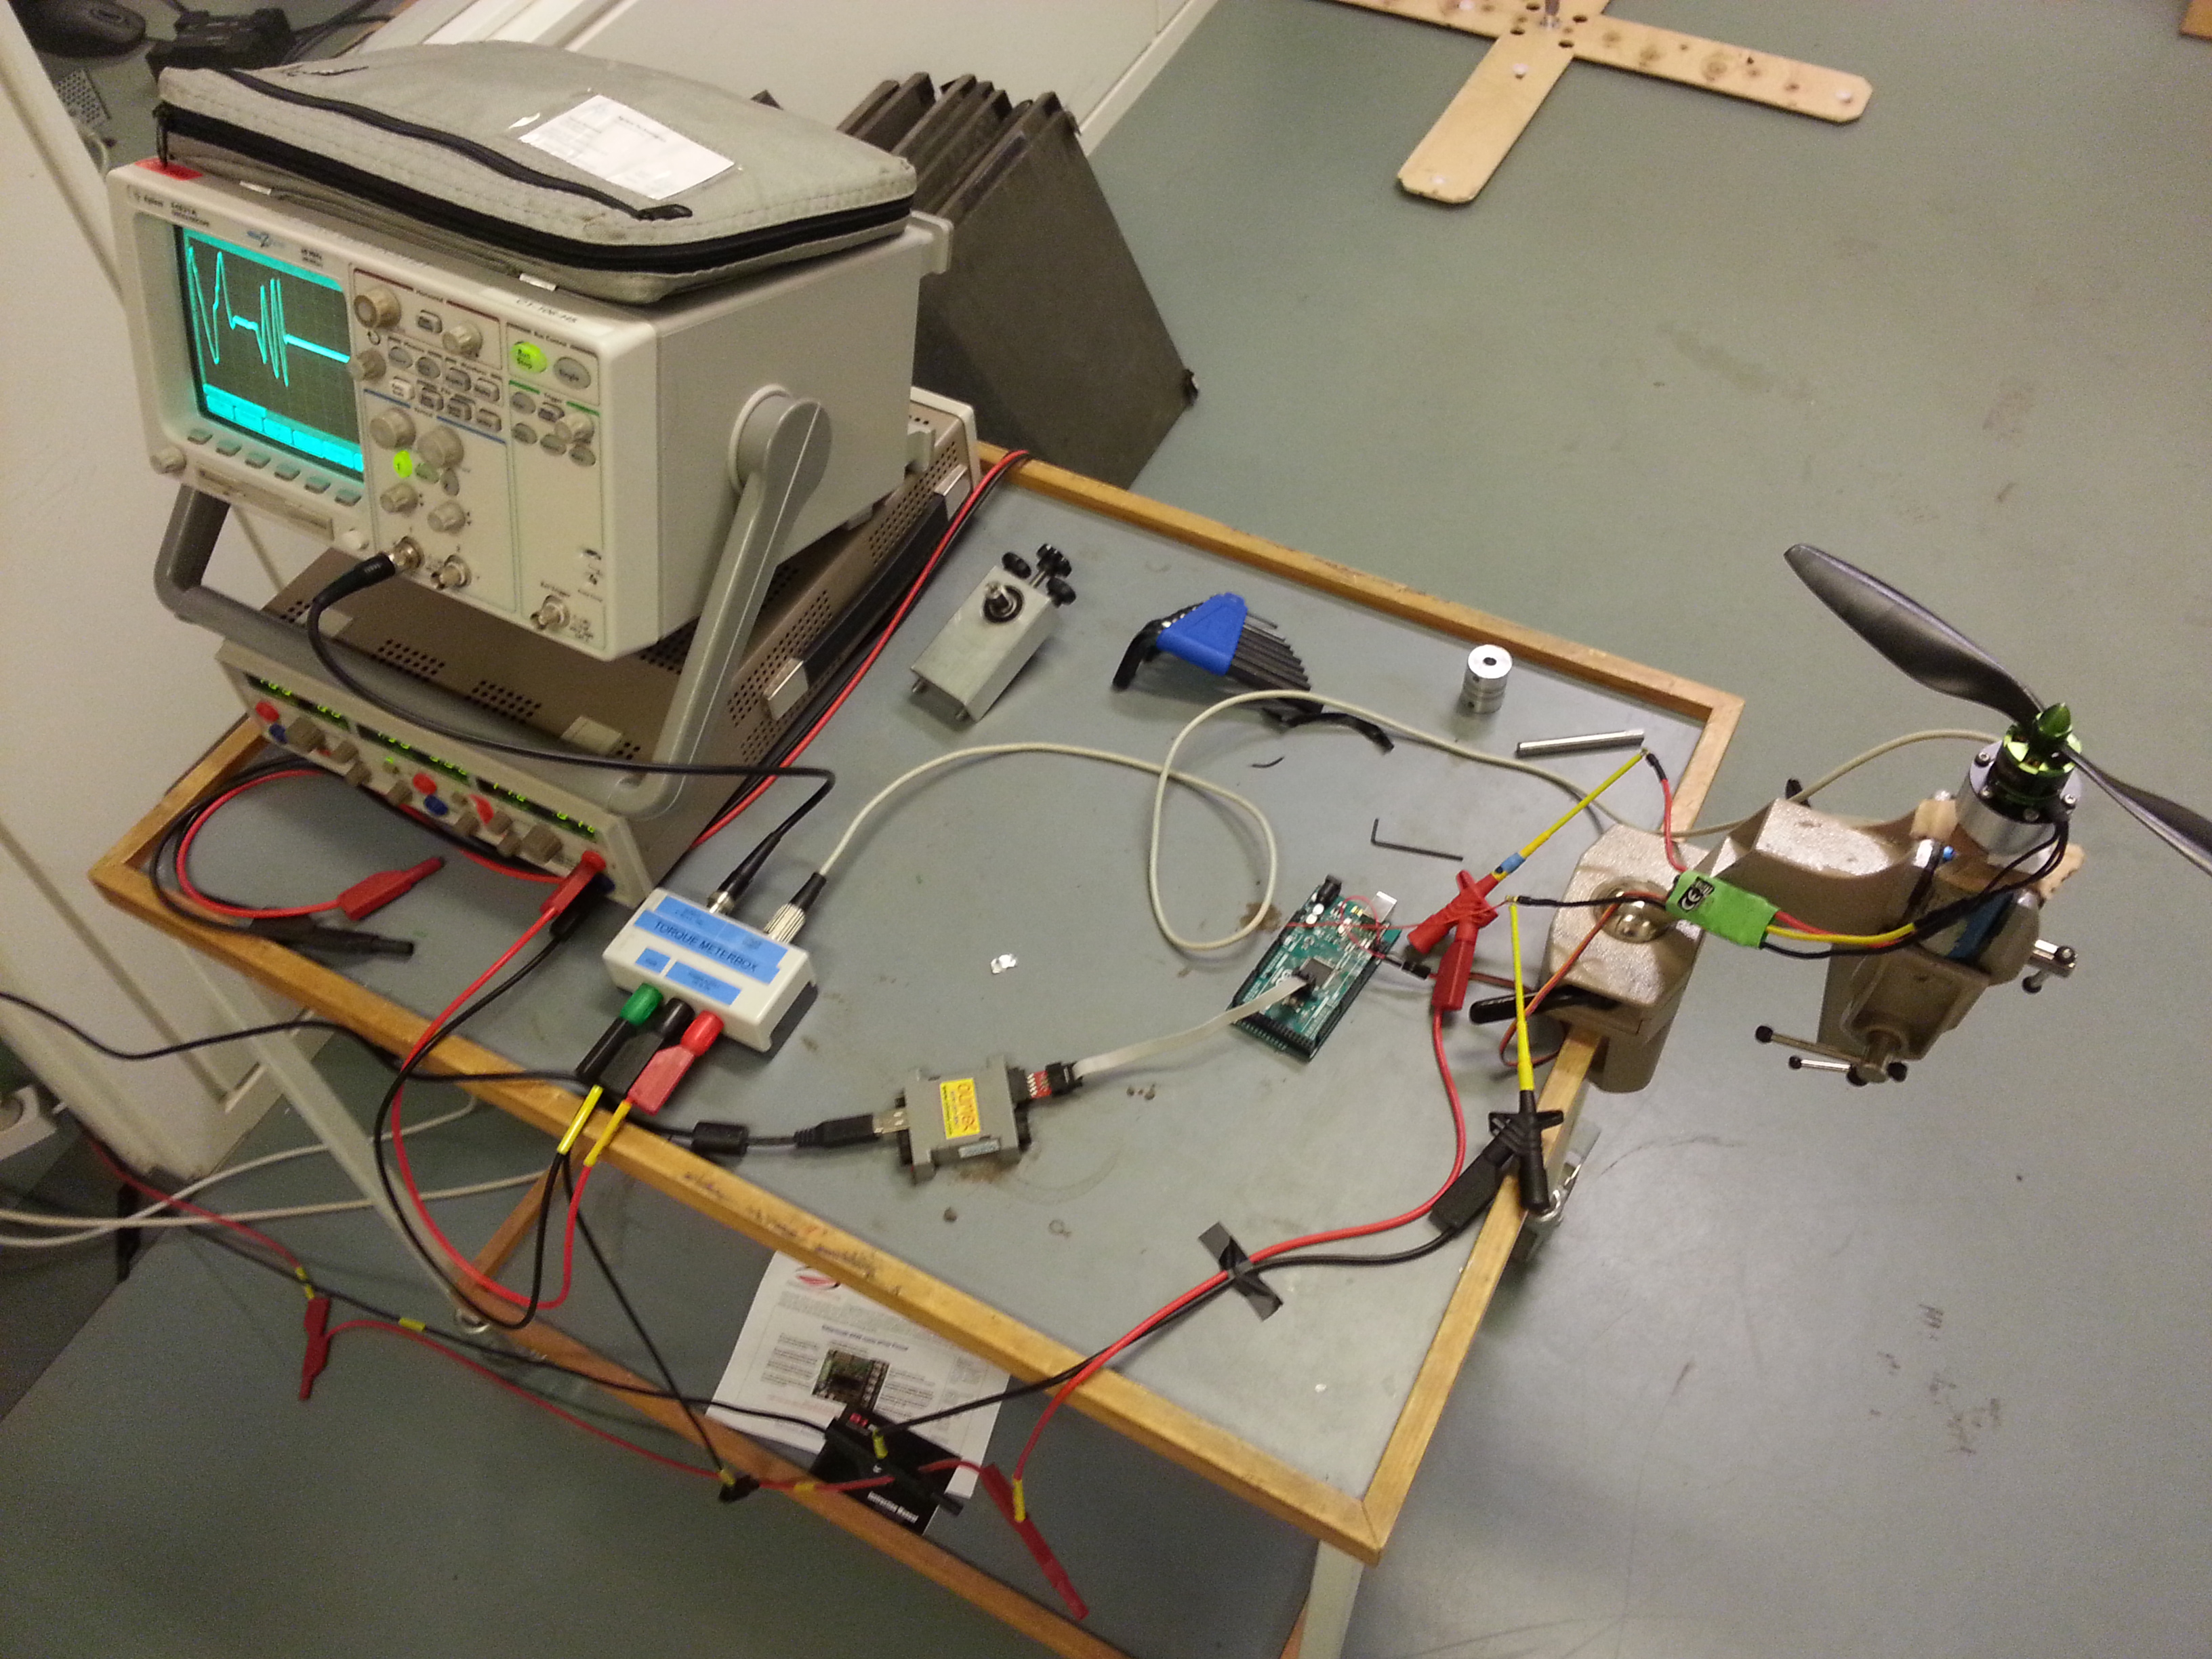
\includegraphics[scale=0.05]{figures/TorqueTestSetup}
	\caption{The setup for the torque test.}
	\label{TorqueTest}
\end{figure}

\subsubsection{List of Equipment}
\begin{table}[H]
	\begin{tabular}{|l|l|p{4.3cm}|}
		\hline%------------------------------------------------------------------------------------------------------------
		\textbf{Instrument}                                  &  \textbf{AAU-no.}  &  \textbf{Type}                       \\
		\hline%------------------------------------------------------------------------------------------------------------
		Tachometer                                           &  08246           &  Shimpo DT-205		                   \\
		\hline%------------------------------------------------------------------------------------------------------------
	    Power Supply (11.1 V) &  64565                   &  ES 030-5                 \\
		\hline%------------------------------------------------------------------------------------------------------------
		Processing Unit                                   &  N/A               & Arduino Mega     \\
		\hline%------------------------------------------------------------------------------------------------------------
		Motor                                         &  N/A               & Multistar 2213-935     \\
		\hline%------------------------------------------------------------------------------------------------------------
		Motor Speed Controller                                   &  N/A               &  -      \\
		\hline%------------------------------------------------------------------------------------------------------------
		Propeller                                   &  N/A               & Turnigy 1045R     \\
		\hline%------------------------------------------------------------------------------------------------------------
		Torquemeter                                   &  N/A               & -     \\
		\hline%------------------------------------------------------------------------------------------------------------
		Oscilloscope                                   & 61604               & Agilent 54621A     \\
		\hline%------------------------------------------------------------------------------------------------------------
		Torquemeter Power Supply                   &  61598              & HM7042-5    \\
		\hline%------------------------------------------------------------------------------------------------------------
		
	\end{tabular}
\end{table}

\subsubsection{Procedure}
\begin{enumerate}
	\item Construct the setup as seen in \figref{TorqueTest}, the power supply is connected to the motor driver and the Arduino Mega is powered from the computer. One PWM pin and GND pin from the board must be connected to the driver signal cables yellow and brown respectively, The torquemeter is connected delivers the measurement as a voltage in the oscilloscope. 
	\item Run the program. It should generate a fixed duty PWM signal in the PWM pin.
	\item Wait for the speed to stabilize and read the torque value as voltage in the oscilloscope. The torque is calculated by considering the the torquemeter specifications. They state that \si{\pm5\textbf{ }V} are equivalent to \si{\pm1\textbf{ }Nm}.
	\item Measure the rotational speed with the tachometer.
\end{enumerate}


\subsubsection{Results}
\begin{table}[H]
	\centering
	\begin{tabular}{|l|l|l|l|p{4.3cm}|}
		\hline%------------------------------------------------------------------------------------------------------------
		\textbf{Motor Speed [rpm]}    & \textbf{Motor Speed [rad/s]} & \textbf{Torque [mV]}  & \textbf{Drag Torque[Nm]} \\ 
		\hline%------------------------------------------------------------------------------------------------------------
		3308 						       &  173,21 				           & 143,8                 & 0,0288         \\
		\hline%------------------------------------------------------------------------------------------------------------
		3416                               &  178,86   			               & 153,1                 & 0,0306         \\
		\hline%------------------------------------------------------------------------------------------------------------
		3655                               &  191,38  			               & 168,8                 & 0,0338         \\
		\hline%------------------------------------------------------------------------------------------------------------
		3755                               &  196,61                           & 171,9                 & 0,0344         \\
		\hline%------------------------------------------------------------------------------------------------------------
		3916 						       &  205,04				           & 206,3                 & 0,0413         \\
		\hline%------------------------------------------------------------------------------------------------------------
		4045                               &  211,80    			           & 212,5                 & 0,0425         \\
		\hline%------------------------------------------------------------------------------------------------------------
		4240                               &  222,01                           & 231,3                 & 0,0463         \\
		\hline%------------------------------------------------------------------------------------------------------------
		4310 						       &  225,67				           & 240,6                 & 0,0481         \\
		\hline%------------------------------------------------------------------------------------------------------------
				
	\end{tabular}
\end{table}
\subsubsection{Results}
The obtained results are shown in \figref{TorqueGraph}. They have been approximated by a parabolic curve by finding a linear relation between the velocity in rad/s squared and the thrust force.

\begin{figure}[H]
	\centering
	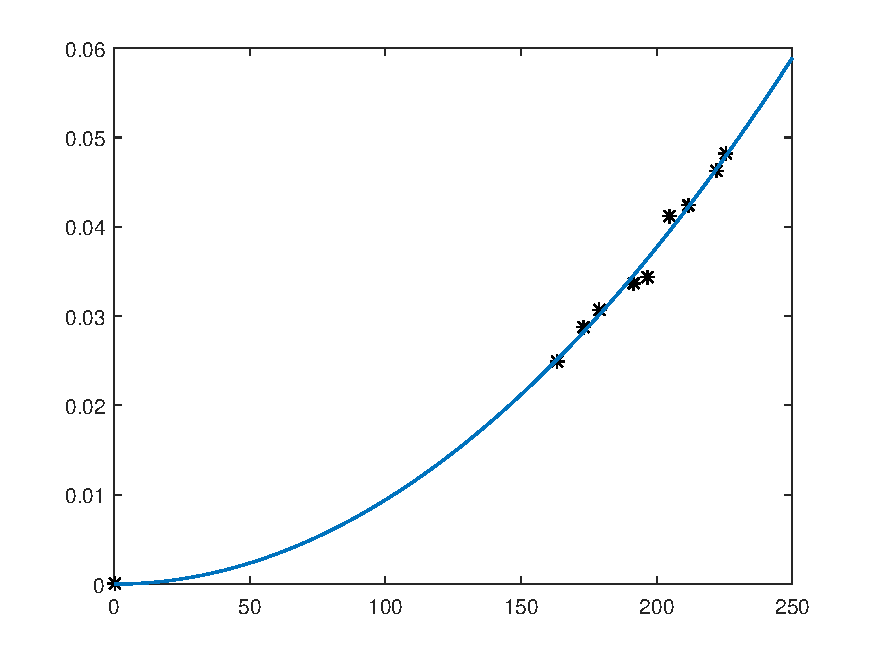
\includegraphics[scale=0.8]{figures/TorqueGraph}
	\caption{Data from the torque test approximated by a parabolic curve.}
	\label{TorqueGraph}
\end{figure}

The resulting constant that provides the relation between the drag torque in the propeller and the velocity squared is \si{9,423327\cdot10^{-7} Nm\cdot s^2/rad^2}.
	
	\chapter{Voltage Level Test}\label{app:VoltageLevelTest} 
\textbf{Name: Group 733}\\
\textbf{Date: 24/10 - 2016}

\subsubsection{Purpose}
Finding the influence of the battery voltage level in the final motor velocity applied by the motor speed controller. The quadcopter controller will account for this influence when setting the speed reference.

\subsubsection{Setup}
%\begin{figure}[H]
%	\centering
%	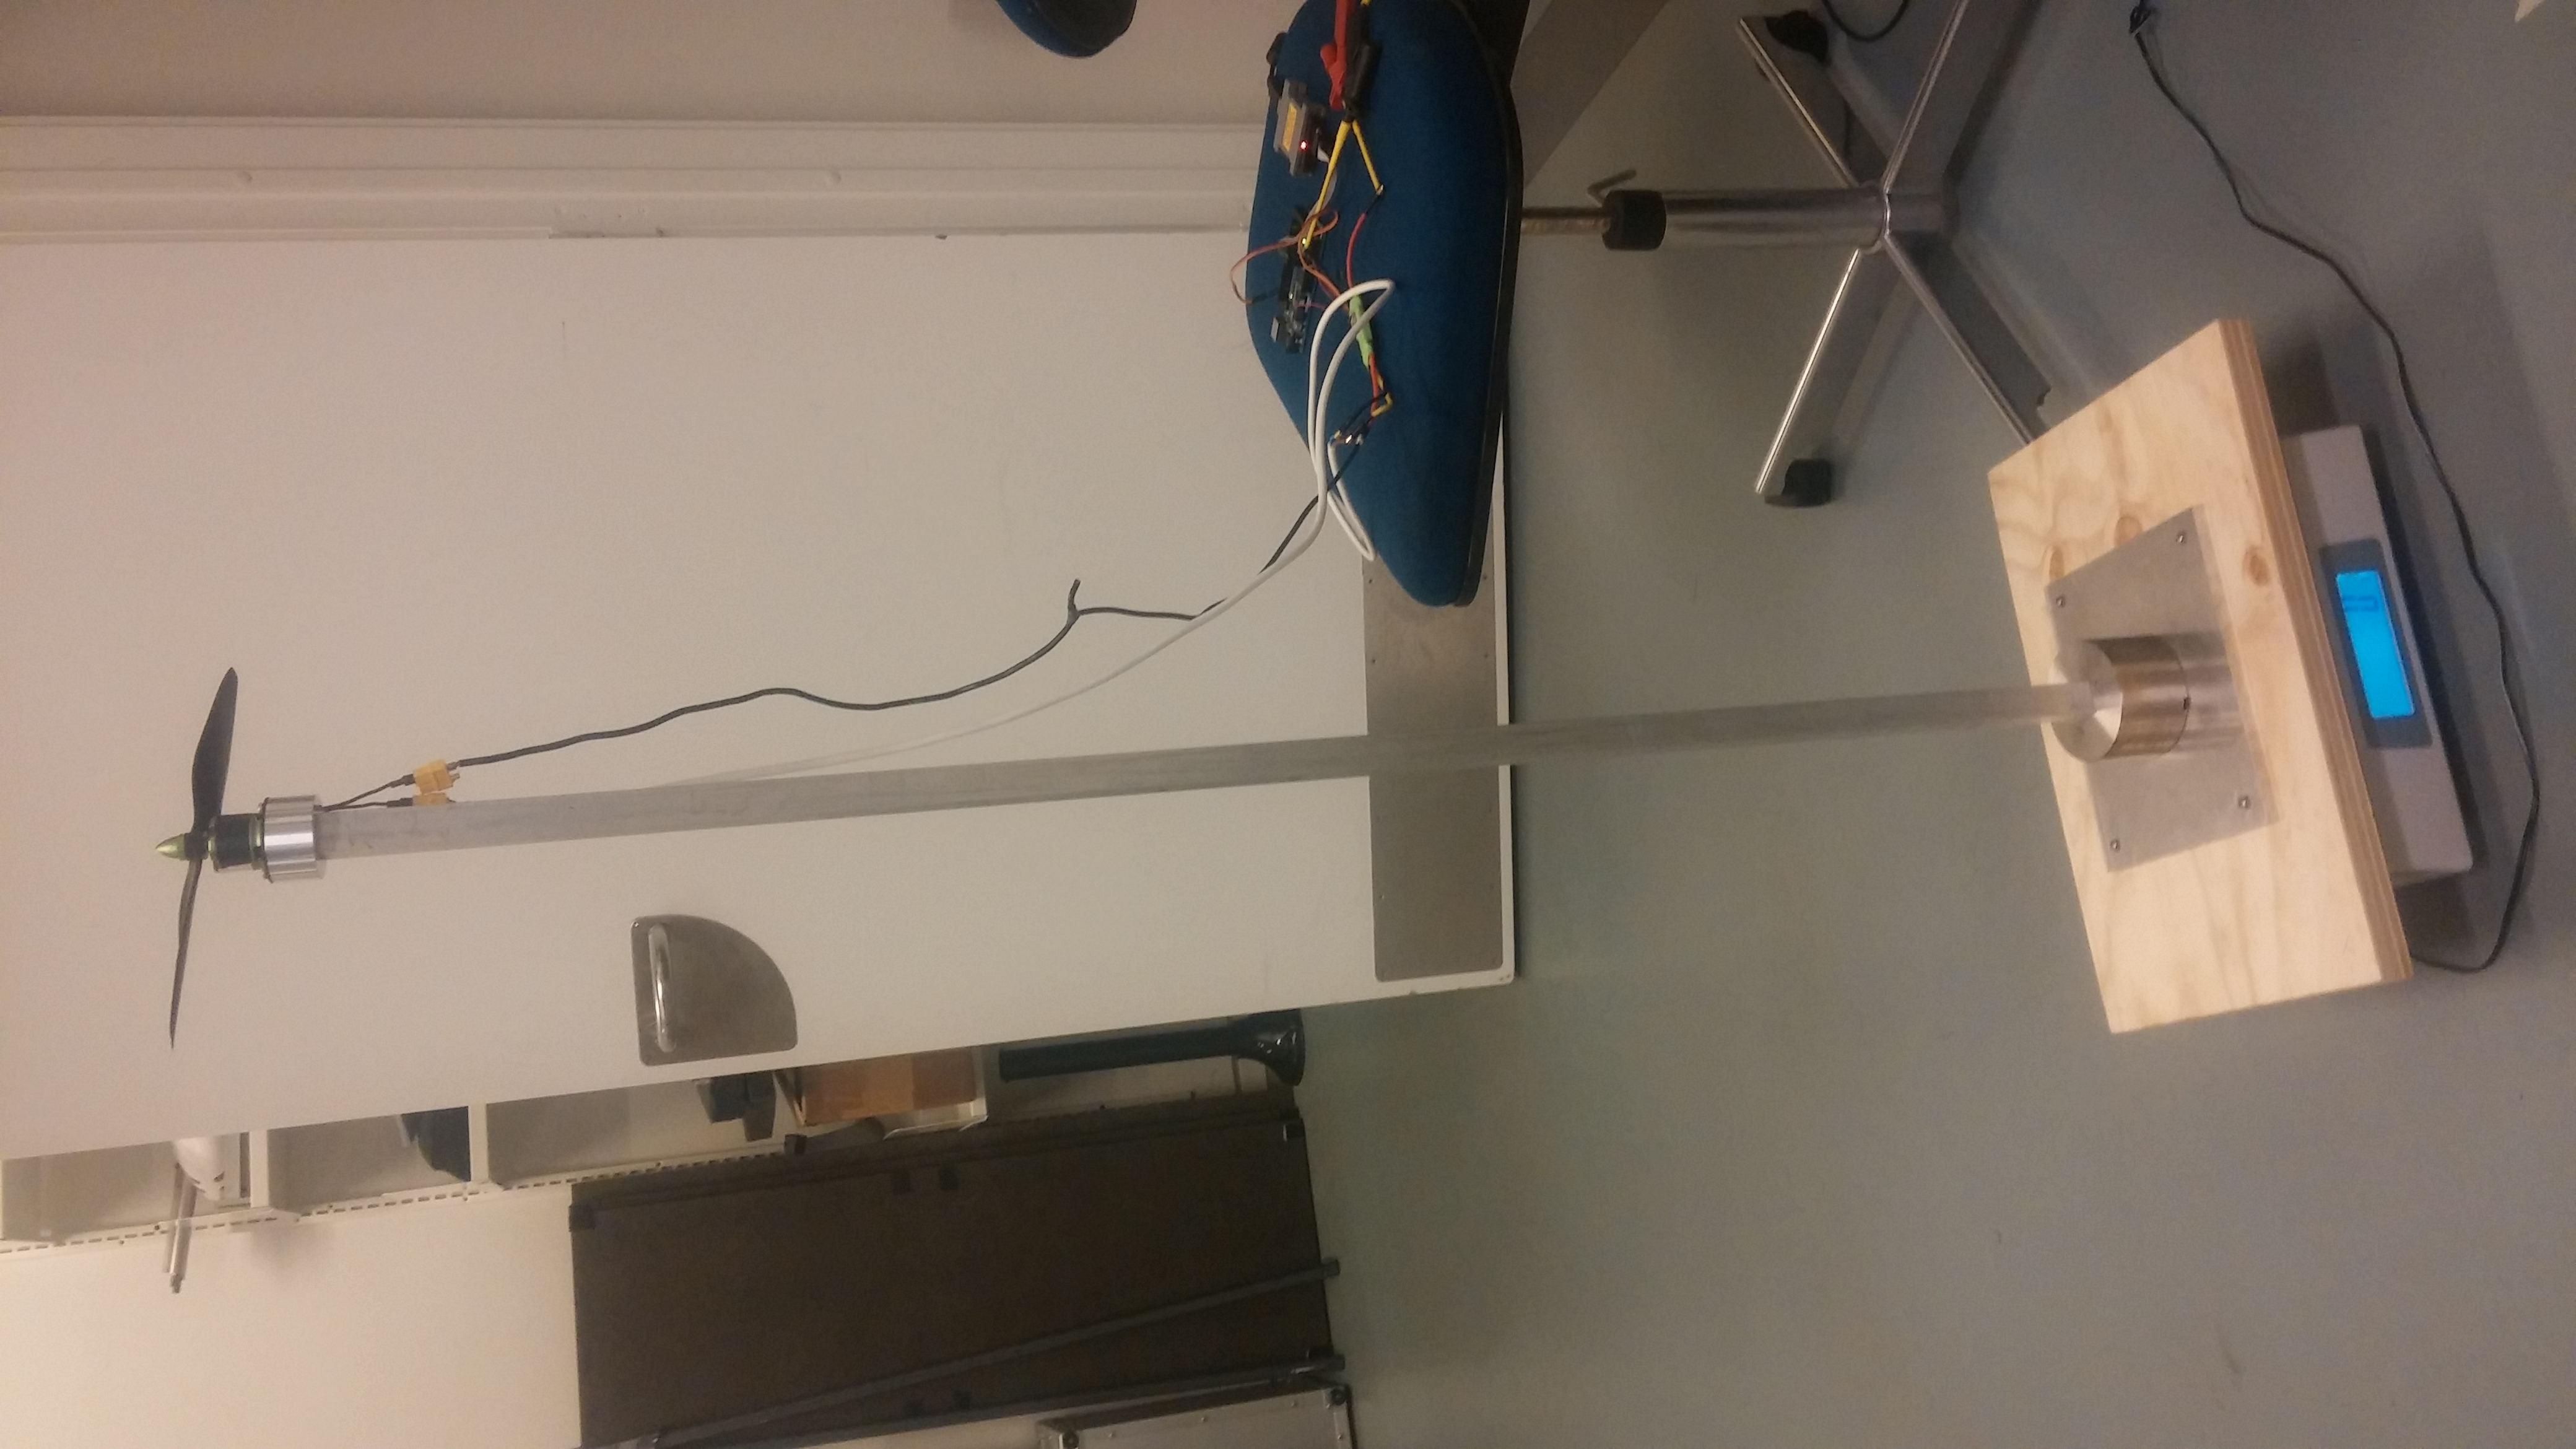
\includegraphics[scale=0.05,angle =-90]{figures/ThrustTestSetup}
%	\caption{The setup for the thrust test.}
%	\label{ThrustTest}
%\end{figure}

\subsubsection{List of Equipment}
\begin{table}[H]
	\begin{tabular}{|l|l|p{4.3cm}|}
		\hline%------------------------------------------------------------------------------------------------------------
		\textbf{Instrument}                          &  \textbf{AAU-no.}  &  \textbf{Type}                       \\
		\hline%------------------------------------------------------------------------------------------------------------
		Tachometer                                   &  08246             &  Shimpo DT-205		                   \\
		\hline%------------------------------------------------------------------------------------------------------------
	    Power Supply (11.1 V)                        &  64565             &  ES 030-5                 \\
		\hline%------------------------------------------------------------------------------------------------------------
		Processing Unit                              &  N/A               & Arduino Mega     \\
		\hline%------------------------------------------------------------------------------------------------------------
		Motor                                        &  N/A               & Multistar 2213-935     \\
		\hline%------------------------------------------------------------------------------------------------------------
		Motor Speed Controller                       &  N/A               &  -      \\
		\hline%------------------------------------------------------------------------------------------------------------
		Propeller                                    &  N/A               & Turnigy 1045R     \\
		\hline%------------------------------------------------------------------------------------------------------------	
	\end{tabular}
\end{table}

\subsubsection{Procedure}
\begin{enumerate}
	\item Construct the setup as seen in \autoref{VoltageTest}, the power supply is connected to the motor driver and the Arduino Mega is powered from the computer. One PWM pin and GND pin from the board must be connected to the driver signal cables yellow and brown respectively. 
	\item Run the program with a fixed PWM duty for each test. Three tests have been performed with duty cycles ir order to check if behaviour is consistent with all speed references.
	\item Wait for the speed to stabilize and measure it with the tachometer. 
	\item Vary the voltage given by the battery and repeat the speed measurement.
\end{enumerate}


\subsubsection{Results}
\begin{table}[H]
	\centering
	\begin{tabular}{|l|l|l|l|p{4.3cm}|}
		\hline%------------------------------------------------------------------------------------------------------------
		\textbf{Voltage Level[V]}    & \textbf{Motor Speed [rpm]} & \textbf{Motor Speed [rad/s]} \\ 
		\hline%------------------------------------------------------------------------------------------------------------
		9.4                & 1393         	   &  145.87                                       \\
		\hline%------------------------------------------------------------------------------------------------------------
		 9.5      &  2111 						       &  221.06				                \\
		\hline%------------------------------------------------------------------------------------------------------------
		 9.6       &  2335                               &  244.52   			                  \\
		\hline%------------------------------------------------------------------------------------------------------------
		9.7    & 2774                               &  290.49  			                       \\
		\hline%------------------------------------------------------------------------------------------------------------
		10   &    2868                               &  300.34                                 \\
		\hline%------------------------------------------------------------------------------------------------------------
		10.2   &  2930 						       &  306.83				                   \\
		\hline%------------------------------------------------------------------------------------------------------------
		10.5 &  3303                               &  317.62    			                    \\
		\hline%------------------------------------------------------------------------------------------------------------
		 10.8   &    3105                               &  325.15                               \\
		\hline%------------------------------------------------------------------------------------------------------------
		11.1     &  3185 						       &  333.53				                \\
		\hline%------------------------------------------------------------------------------------------------------------
	\end{tabular}
	\caption{Results obtained when applying a duty cycle of 170 out of 256 in the motor speed reference.}
\end{table}
\begin{table}[H]
	\centering
	\begin{tabular}{|l|l|l|l|p{4.3cm}|}
		\hline%------------------------------------------------------------------------------------------------------------
		\textbf{Voltage Level[V]}    & \textbf{Motor Speed [rpm]} & \textbf{Motor Speed [rad/s]} \\ 
		\hline%------------------------------------------------------------------------------------------------------------
		9.4                & 1558         	   &  163.15                                       \\
		\hline%------------------------------------------------------------------------------------------------------------
		9.5      &  1938 						       &  202.95				                \\
		\hline%------------------------------------------------------------------------------------------------------------
		9.6       &  2431                               &  254.57   			                  \\
		\hline%------------------------------------------------------------------------------------------------------------
		9.7    & 2785                               &  291.64  			                       \\
		\hline%------------------------------------------------------------------------------------------------------------
		10   &    3251                               &  340.44                                 \\
		\hline%------------------------------------------------------------------------------------------------------------
		10.2   &  3274 						       &  342.65				                   \\
		\hline%------------------------------------------------------------------------------------------------------------
		10.5 &  3361                               &  351.96    			                    \\
		\hline%------------------------------------------------------------------------------------------------------------
		10.8   &    3444                               &  360.65                               \\
		\hline%------------------------------------------------------------------------------------------------------------
		11.1     &  3484 						       &  364.84				                \\
		\hline%------------------------------------------------------------------------------------------------------------
	\end{tabular}
	\caption{Results obtained when applying a duty cycle of 170 out of 256 in the motor speed reference.}
\end{table}
\begin{table}[H]
	\centering
	\begin{tabular}{|l|l|l|l|p{4.3cm}|}
		\hline%------------------------------------------------------------------------------------------------------------
		\textbf{Voltage Level[V]}    & \textbf{Motor Speed [rpm]} & \textbf{Motor Speed [rad/s]} \\ 
		\hline%------------------------------------------------------------------------------------------------------------
		9.4                & 1428         	   &  149.54                                       \\
		\hline%------------------------------------------------------------------------------------------------------------
		9.5      &  1853 						       &  194.05				                \\
		\hline%------------------------------------------------------------------------------------------------------------
		9.6       &  2543                               &  266.30   			                  \\
		\hline%------------------------------------------------------------------------------------------------------------
		9.7    & 2772                               &  290.283  			                       \\
		\hline%------------------------------------------------------------------------------------------------------------
		10   &    3423                               &  358.46                                 \\
		\hline%------------------------------------------------------------------------------------------------------------
		10.2   &  3509 						       &  367.46				                   \\
		\hline%------------------------------------------------------------------------------------------------------------
		10.5 &  3610                               &  378.04    			                    \\
		\hline%------------------------------------------------------------------------------------------------------------
		10.8   &    3675                               &  384.85                               \\
		\hline%------------------------------------------------------------------------------------------------------------
		11.1     &  3745 						       &  392.18				                \\
		\hline%------------------------------------------------------------------------------------------------------------
	\end{tabular}
	\caption{Results obtained when applying a duty cycle of 170 out of 256 in the motor speed reference.}
\end{table}
\subsubsection{Results}
The obtained results are represented in \autoref{VoltageGraph}. As it can be seen, the motor speeds follow a linear trend for voltages above 10 V and drop fast for lower voltages. The line used for compensating this effect is calculated as the average of those obtained in the experiments, considering only the linear region
%\begin{figure}[H]
%	\centering
%	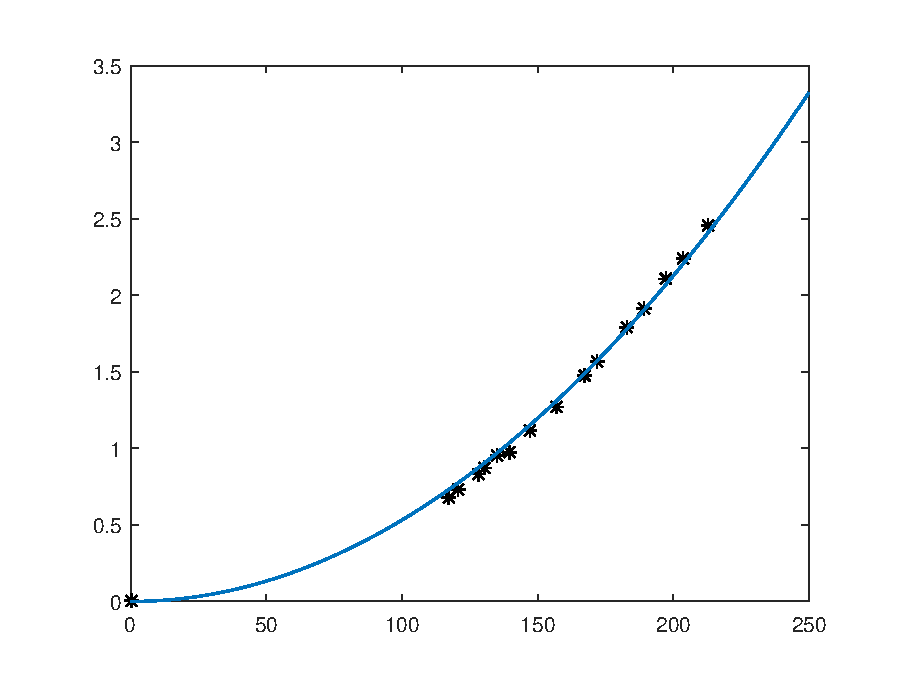
\includegraphics[scale=0.8]{figures/ThrustGraph}
%	\caption{Data from the thrust test approximated by a parabolic curve.}
%	\label{ThrustGraph}
%\end{figure}
The resulting FINISH THIS.
	
%	\end{appendices}
		
	%%% Bibliography %%%
	\printbibliography
	
	%%% To Do List %%%

	\end{document}
